\documentclass[german, parskip=full, 12pt]{article}
\usepackage{setup}
 


% automatischen Titel konfigurieren
\begin{document}

\title{\vspace{3cm}
\titel \\
\vspace{2cm}
 \Large inoffizielles Vorlesungsskript
 \vspace{5cm}
 }


\author{\betreuer}
\date{Wintersemester 2023/2024}



\maketitle
\newpage

\tableofcontents
\newpage

\include{1_Einführung}

\section{Grundlagen der statistischen Physik}
\subsection{Mikrozustand, Makrozustand, statistisches Ensemble}

\begin{definition}{Mikrozustand}
    Ein Zustand bei dem sämtliche Information über das System bekannt ist.
    \begin{itemize}
        \item qm: \ Zustand $\ket{\Psi}$, Vektor im Hilbert-Raum 
        \item klass.: \ Orte und Impulse aller Teilchen 
    \end{itemize}
\end{definition}

\begin{beispiel}{Beispiel}
    \begin{itemize}
    \item Elektron mit $z^+$ Spin (vgl. Stern-Gerlach-Experiment)
    \item Grundzustand im \textbf{HO} (Harmonischen Oszillator)
    \item Superposition von 2. + 3. angeregten Zustand: $ \frac{1}{\sqrt{2}}(\ket{2} + \ket{3})$
    \item System von 100 Spins: $\underbrace{\text{1. Spin } z^+\text{, 2.Spin } x^-, \dots, \text{ 100. Spin } y^+}_{\text{Superpositionen}}$
 \end{itemize}
\end{beispiel}



\begin{definition}{Makrozustand}
    Das System wird durch makroskopische Größen (Gesamtenergie, Magnetisierung, Entropie) beschrieben, wobei die Details über den zugrundeliegenden Mikrozustand unbekannt sind und dieser auch \textbf{nicht messbar} ist (meist auch nicht nötig). Viele Mikrozustände führen zu dem gleichen Makrozustand. Es ist aber möglich, statistische Aussagen über den Mikrozustand zu treffen.
\end{definition}

\begin{beispiel}{Beispiel statistische Aussage:}
Zustand $\ket{\Psi}$ mit \textbf{WS} (Wahrscheinlichkeit) $w_m$, wobei gilt: $\forall m: w_m \geq 0 \wedge \sum_m w_m = 1 \quad (\Rightarrow \forall m: w_m \leq 1)$
\end{beispiel}
 
\begin{definition}{Statistisches Ensemble}
    Man denkt sich eine große Menge von Kopien des Systems, die alle den gleichen Makrozustand haben. Jede dieser Kopien ist in einem Mikrozustand $\ket{\Psi_n}$ mit WS $w_n$.\\ $\Rightarrow$ wesentlich mehr Kopien als Anzahl Mikrozustände
\end{definition}

\subsection*{Ziel der statistischen Physik}
\begin{itemize}
    \item Theorie für WS $w_n$
    \item basierend auf \glqq sinnvollen\grqq \, Annahmen
    \item experimentelle Aussagen
\end{itemize}


\subsection{Dichteoperator (statistischer Operator)}     \marginpar{VL 2}

Wie beschreibt man einen Makrozustand / statistisches Ensemble?

\vspace{0.5cm}
\underline{Idee}
\begin{itemize}
    \item [$\rightarrow$] Superposition: $\sum_n w_n \ket{\Psi_n}$ \textbf{nicht richtig}: immer noch Mikrozustand, nur normiert für $w_n \rightarrow \sqrt{w_n}$, falsche Aussagen für Messungen
\end{itemize}

\begin{beispiel}{Beispiel: polarisiertes Licht}
    \begin{itemize}
    \item Makrozustand: 50 \% $\updownarrow$, 50 \% $\leftrightarrow$
    \item Messung mit $\nearrow$ Polarisator: 50 \% Intensität (jede Polarisationsrichtung lässt 50 \% Intensität durch (2 * 0.5 * 50 \% = 50 \%)
    \item falsche Beschreibung: Superposition: $\frac{1}{\sqrt{2}} ( \ket{\updownarrow} + \ket{\leftrightarrow}) = \ket{\nearrow}$
    \item[$\Rightarrow$] 100 \% Intensität
\end{itemize}
\end{beispiel}



\begin{definition}{Dichteoperator}
    \begin{equation}
        \hat{\varrho} := \sum_n w_n \ket{\Psi_n} \bra{\Psi_n}
    \end{equation}

    \begin{itemize}
        \item $\ket{\Psi_n}$ müssen normiert sein: $\bra{\Psi_n}\ket{\Psi_n} = 1$
        \item $\ket{\Psi_n}$ müssen nicht orthogonal sein (z.B.: 20\% $\updownarrow$, 80\% $\leftrightarrow$)
        \item $\sum_n \rightarrow \int dn$ , falls kontinuierlich
    \end{itemize}
\end{definition}

$\ket{\Psi_n}\bra{\Psi_n}$ ist \underline{Projektionsoperator}
\begin{definition}{Projektionsoperator}
\begin{equation}
    P^2 = P
\end{equation}
\end{definition}



\begin{proof}
\begin{equation}
    \ket{\Psi}\underbrace{\bra{\Psi}\ket{\Psi}}_{=1}\bra{\Psi} = \ket{\Psi}\bra{\Psi}
\end{equation}
$\ket{\Psi}\bra{\Psi}$ ist Projektionsoperator.

\end{proof}

$P = \ket{\Psi}\bra{\Psi}$ projiziert auf Zustand $\ket{\Psi}$

\begin{proof}
    \begin{equation}
        P \ket{\varphi} = \ket{\Psi} \bra{\Psi} \ket{\varphi} = \bra{\Psi}\ket{\varphi}\ket{\Psi} \ \  \parallel \ket{\Psi}
    \end{equation}
\end{proof}

\subsubsection{Reine Zustände}
 System sei in normierten Zustand $\ket{\Psi}$ ($\bra{\Psi}\ket{\Psi} = 1$). Ziel: Vorhersagen für Messung einer Observablen $A$:
 \begin{itemize}
     \item Eigenwertgleichung zu selbstadjunggierten\footnote{In der Vorlesung wird diese Eigenschaft anscheinend fälschlicher Weise als "hermitesch" bezeichnet.} Operator $A$: \ \ $A^{\dag} = A$
     \begin{equation}
         A \ket{\alpha_k} = a_k \ket{\alpha_k}
     \end{equation}
     \item Eigenwerte $a_k$ sind mögliche Messergebnisse
     \item Eigenzustände $\ket{\alpha_k}$
    \begin{itemize}
         \item[-] orthonormiert: $\bra{\alpha_l}\ket{\alpha_k} = \delta_{l,k}$
         \item[-] vollständig: $\sum_k \ket{\alpha_k}\bra{\alpha_k} = \mathds{1}$ \makebox(0,0){\put(0,2.2\normalbaselineskip){%
               $\left.\rule{0pt}{1.1\normalbaselineskip}\right\}$ $\{ \ket{\alpha_k}\}$ ist VONS}}
     \end{itemize}
     \item Zustand $\ket{\Psi}$ entwickeln in $\ket{\alpha_k}$:
         \begin{equation}
             \ket{\Psi} = \sum_k c_k \ket{\alpha_k} \ \ \ \text{mit} \ c_k = \bra{\alpha_k}\ket{\Psi}
         \end{equation}
    \begin{proof}
        \begin{equation}
            \ket{\Psi} = \underbrace{\sum_k \ket{\alpha_k}\bra{\alpha_k}}_{= \mathds{1}} \ket{\Psi} = \ket{\Psi}
        \end{equation}
    \end{proof}
    \item Messung von $A$ ergibt Eigenwert $a_k$ mit WS $p_k = \left|c_k \right| ^2 = \left| \bra{\alpha_k}\ket{\Psi}\right|^2$ (\emph{Born'sche Regel})
    \begin{proof}
        \begin{equation}
            \sum_k p_k = \sum_k \braket{\Psi}{\alpha_k}\braket{\alpha_k}{\Psi} = \bra{\Psi}\underbrace{\sum_k \ket{\alpha_k}\bra{\alpha_k}}_{= \mathds{1}} \ket{\Psi} = \braket{\Psi}{\Psi} = \mathds{1}
        \end{equation}
    \end{proof}
    \item \underline{Erwartungswert} von $A$ für Zustand $\ket{\Psi}$:
    \begin{equation}
        \langle A \rangle := \bra{\Psi}A\ket{\Psi} = \sum_k \bra{\Psi}A\ket{c_k \alpha_k} = \sum_k c_k a_k \underbrace{\braket{\Psi}{\alpha_k}}_{c_k^*} = \sum_k \left| c_k \right|^2 a_k = \sum_k p_k a_k
    \end{equation}

 \end{itemize}
 
Die WS $p_k$ sind rein qm Natur. Mit ihnen kann man die WS für Messergebnisse $a_k$ vorhersagen.

\textbf{Achtung: falsche Aussage:} \glqq System ist mit WS $p_k$ im Zustand $\ket{a_k}$ \grqq $\rightarrow$ System kollabiert bei Messung in Eigenzustand (vgl. QM I)

\subsubsection*{Dichteoperator}
äquivalentes Konzept für reinen Zustand $\ket{\Psi}$, $\hat{\varrho} = \ket{\Psi} \bra{\Psi}$

\begin{equation}
    \Rightarrow p_k = |\braket{a_k}{\Psi}|^2 = \braket{a_k}{\Psi}\braket{\Psi}{a_k} = \bra{a_k} \hat{\varrho} \ket{a_k}
\end{equation}
\begin{align}
    \langle A \rangle = \bra{\Psi} A \ket{\Psi} = \sum_k c_k \bra{\Psi} A \ket{a_k} = \sum_k \braket{a_k}{\Psi} \bra{\Psi} A \ket{a_k} = \underbrace{\sum_k \bra{a_k} \hat{\varrho} A \ket{a_k}
    = \trace \hat{\varrho} A}_{\text{da $\ket{a_k}$ VONS}}
\end{align}

\underline{Vorteile des Dichteoperators (reine Zustände):}
\begin{itemize}
    \item beliebiger Phasenfaktor in $\ket{\Psi}$, aber nicht in $\hat{\varrho} = \ket{\Psi} \bra{\Psi}$
    \item $\langle A \rangle$ ist linear in $\hat{\varrho}$, aber quadratisch in $\ket{\Psi}$
\end{itemize}

\subsubsection*{Eigenschaften der Spur}
\begin{definition}{Spur}
    \begin{equation}
        \trace X := \sum_n \bra{\varphi_n}X\ket{\varphi_n} \ \ \ \text{ mit bel. VONS } \{\ket{\varphi_n}\} \text{ (von Basis unabhängig)}
    \end{equation}
    \begin{align}
        \trace (X+Y) &= \trace X + \trace Y  \\ 
        \trace(cX) &= c \cdot \trace X  \ \ c \in \mathbb{C} \\
        \trace (XY) &= \trace(YX) \   \Rightarrow \ \trace(XYZ) = \trace(YZX) = \trace (ZXY) \text{ zyklisch!} \\
        \trace (X^{\dag}) &= (\trace X)^* \\
        \trace(\ket{\varphi}\bra{\Psi}) &= \braket{\Psi}{\varphi}
    \end{align}
\end{definition}

\subsubsection{gemischte Zustände}
Makrozustand (Ensemble) vieler möglicher Mikrozustände $\ket{\Psi_n}$ mit WS $w_n$ ($w_n \geq 0, \sum_n w_n = 1, \ket{\Psi_n} \text{ normiert, i.A. nicht orthogonal})$

$\rightarrow$ alle Informationen aus Dichteoperator bestimmbar:
\begin{itemize}
    \item WS für Messergebnis $a_k$:
    \begin{align}
        p_k &= \sum_n w_n |\braket{a_k}{\Psi_n}|^2 \quad \text{\glqq Mitteln über Mikrozustände \grqq} \\
        &= \sum_n w_n\bra{a_k} \ket{\Psi_n} \bra{\Psi_n} \ket{a_k} \\
        &= \bra{\alpha_k} \underbrace{\sum_n w_n \ket{\Psi_n}\bra{\Psi_n}}_{=\varrho} \ket{\alpha_k} = \bra{a_k} \hat{\varrho} \ket{a_k}
    \end{align}
    \item Erwartungswert von A:
    \begin{align}
        \langle A \rangle &= \sum_n w_n \underbrace{\bra{\Psi_n} A \ket{\Psi_n}}_{\trace () \text{, da nur komplexe Zahl}} \\
        &= \sum_n w_n \trace(\ket{\Psi_n} \bra{\Psi_n} A )\\
        &= \trace \bigl(\sum_n w_n \ket{\Psi_n} \bra{\Psi_n} A \bigr) = \trace( \hat{\varrho} A)
    \end{align}

    \begin{equation}
        \fcolorbox{red}{white}{$\langle A \rangle = \trace( \hat{\varrho} A)$}
    \end{equation}
\end{itemize}

Verschiedene $\{ \ket{\Psi_n}, w_n \}$ können zu gleichen $\varrho$ führen.
Sie beschreiben den gleichen Makrozustand.
Kein Experiment kann (im Rahmen der Quantenmechanik) einen Unterschied finden!


\begin{prop}{Eigenschaften von $\varrho$}
 \begin{equation*}
     \begin{rcases*}
        &\qq{1.}  $\varrho^{\dag} = \varrho \ $ selbstadjungiert\footnote{laut Ketzmerick "hermitesch"}\\
        &\qq{2.} $\trace \varrho = 1$ \\
        &\qq{3.} \text{Positivität } \forall \ket{\varphi}: \; \bra{\varphi} \varrho \ket{\varphi} \geq 0 \;\\
        &\qquad \Leftrightarrow \text{ alle Eigenwerte } \geq 0
    \end{rcases*} \Leftrightarrow \varrho \quad \text{ist Dichteoperator} 
 \end{equation*}
\end{prop} 

\newpage
 \subsubsection*{Unterschiede zwischen reinen und gemischten Zuständen}
\begin{multicols}{2}
 \underline{reiner Zustand}
 \begin{itemize}
     \item $\varrho ^2 = \varrho$
     \begin{proof}
         $\varrho ^2 = \ket{\Psi} \underbrace{\braket{\Psi}}_{\mathds{1}} \bra{\Psi} = \varrho$
     \end{proof}
     \item $\trace \varrho^2 =1$
 \end{itemize}
 \columnbreak
 \underline{gemischter Zustand (nicht reiner Zustand)}
 \begin{itemize}
     \item $\varrho ^2 \neq \varrho$
     \item $\trace\varrho^2 < 1$
     \item[] 
     \item[]
 \end{itemize}
\end{multicols}
\subsubsection{Dichtematrix}

\begin{definition}{Dichtematrix in bel. VONS $\{ \ket{\Phi_k}\}$}
    \begin{equation}
        \varrho_{lk} := \bra{\Phi_k} \hat{\varrho} \ket{\Phi_l}
    \end{equation}
    
\end{definition}

\begin{itemize}     \marginpar{VL 3}
    \item Kenntnis aller Matrixelemente enthält volle Information
    \item wähle als Basis $\{\ket{\alpha_k}\}$ (Eigenzustände der Observablen A: \ $A \ket{\alpha_k} = a_k \ket{\alpha_k}$)
    \item [$\Rightarrow$] physikalische Bedeutung
    \begin{itemize}
        \item Diagonalelemente $\varrho_{kk} = \bra{\alpha_k} \varrho \ket{\alpha_k} \stackrel{s.o.}{=} p_k \geq 0$ (Besetzung)\\
        Dies ist die Wahrscheinlichkeit, $a_k$ zu messen.
        \item $\varrho_{kk} = p_k$ enthält zwei Wahrscheinlichkeitsaussagen:
        \begin{enumerate}
            \item die quantenmechanische für reine Zustände (vgl. \emph{Born'sche Regel})
            \item die statistische aufgrund unvollständiger Information über das System 
        \end{enumerate}
        \item Nicht-Diagonalelemente $\varrho_{kl}$:  $\varrho_{kl} = \bra{\alpha_k} \varrho \ket{\alpha_l} = \sum_n w_n \bra{\alpha_k}\ket{\Psi_n}\bra{\Psi_n}\ket{\alpha_l}$ (Kohärenz [gibt Aussage über Phasenbeziehungen])
    \end{itemize}
\end{itemize}

\begin{beispiel}{Teilchen im Potential (H.O:) mit Eigenzuständen $\ket{n}$:}
$H\ket{n} = E_n \ket{n}$
\begin{itemize}
    \item[a)] reiner Zustand: 
    \begin{align}
        \ket{\Psi} &= \frac{1}{\sqrt{2}} \left( \ket{0} + \ket{1} \right) \\
        \Hat{\varrho} &= \ket{\Psi}\bra{\Psi} = \left( \frac{1}{\sqrt{2}} ( \ket{0} + \ket{1}) \right) \left(\frac{1}{\sqrt{2}} ( \bra{0} + \bra{1}) \right) \\
        &= \frac{1}{2}(\ket{0}\bra{0} + \ket{0}\bra{1} + \ket{1}\bra{0} + \ket{1}\bra{1})
    \end{align}
    \item[] Dichtematrix in der Basis $\{ \ket{n} \}$:
    \begin{equation}
        (\varrho)_{\{ \ket{n} \}} = (\varrho) = \begin{pmatrix}
            \frac{1}{2} & \frac{1}{2} & 0 & 0 & \dots \\
            \frac{1}{2} & \frac{1}{2} & 0 & 0 & \dots \\
            0 & 0 & 0 & 0 & \dots \\
            \vdots & \vdots & \vdots & \vdots & \ddots
            \end{pmatrix}
    \end{equation}
    \item[b)] gemischter Zustand: mit WS $\frac{1}{2}$ in $\ket{0}$ und mit WS $\frac{1}{2}$ in $\ket{1}$
    \begin{align}
        \varrho &= \frac{1}{2} \ket{0}\bra{0} + \frac{1}{2} \ket{1}\bra{1}
    \end{align}
    \item[] Dichtematrix in der Basis $\{ \ket{n} \}$:
    \begin{equation}
        (\varrho)_{\{ \ket{n} \}} = (\varrho) = \begin{pmatrix}
            \frac{1}{2} & 0 & 0 & 0 & \dots \\
            0 & \frac{1}{2} & 0 & 0 & \dots \\
            0 & 0 & 0 & 0 & \dots \\
            \vdots & \vdots & \vdots & \vdots & \ddots
        \end{pmatrix}
    \end{equation}
\end{itemize}
\end{beispiel}





$\Longrightarrow$ \textbf{Wie unterscheiden sich a) und b) bei der Messung?}

\subsubsection{Messung}
\begin{itemize}
    \item[] Observable A mit $A \ket{\alpha_k} = a_k \ket{\alpha_k}$
    \item[] Projektor\footnote{Projektoren haben immer Eigenwerte 0 und 1.} auf Zustand $\ket{\alpha_k}$: $P_k = \ket{\alpha_k}\bra{\alpha_k}$
    \item[] WS $a_k$ zu messen:
    \begin{equation*}
        p_k = \trace(P_k \varrho) = \sum_l \underbrace{\bra{\alpha_l}\ket{\alpha_k}}_{\delta_{kl}} \bra{\alpha_k} \varrho \ket{\alpha_l} = \bra{\alpha_k} \varrho \ket{\alpha_k} = \varrho_{kk}
    \end{equation*}
\end{itemize}

Dichteoperator nach Messung von $a_k$:
\begin{equation}
    \hat{\varrho}' = \frac{P_k \varrho P_k}{\trace(P_k \varrho P_k)} = \frac{P_k \varrho P_k}{\trace(P_k P_k \varrho)} = \frac{P_k \varrho P_k}{p_k} = \frac{\ket{\alpha_k} \bra{\alpha_k} \varrho \ket{\alpha_k} \bra{\alpha_k}}{\bra{\alpha_k} \varrho \ket{\alpha_k}} = \ket{\alpha_k} \bra{\alpha_k}
\end{equation}
$\Longrightarrow$ entspricht Postulat der QM zur Messung\\

Reiner Zustand: 
\begin{itemize}
    \item unabhängig von $\varrho$
    \item abhängig von A und Messergebnis
\end{itemize}

\subsubsection*{Vergleich Beispiele a) und b)\footnote{\textbf{Tangente aus Kais Übung:} \\ a) ist ist quantemnechanische Superposition wie bei Schödingers Katze: Katze ist gleichzeitig im Zustand lebendig und im Zustand tod.\\ b) klassischer Fall: entweder ein ZUstand oder der andere. \\ Unterschied zwischen klassischer Unsicherheit und quantenmechanischen Superposition steckt in Nebendiagonalen. \\Wie kommt man von quantenmechanischer Superposition zu klassischem Gemisch, das wir im ALltag beobachten? Antwort gibt die Theorie der offenen Quantensysteme (Betrachtung der Umgebung- Einfluss der Dekohärenz zerstören Nebendiagonalen). \\
Wie bereits bekannt können verschiedene Mikrozustände zum gleichen Dichteoperator führen (Siehe Blatt 2): \\ Intuition: Dichteoperator zeigt auch nichti}}
\begin{itemize}
    \item Messung Energie mit H: $H \ket{n} = E_n \ket{n}$ z.B. $ n = 0$
    \begin{equation}
        p_0 = \bra{0} \varrho \ket{0} = \varrho_{00} = \begin{cases}
            \frac{1}{2} & \text{, in a)} \\
            \frac{1}{2} & \text{, in b)}
        \end{cases}
    \end{equation}
    \item[$\rightarrow$] gleich, da Diagonale der Dichtematrix zur Basis $\{\ket{n}\}$ gleich
    \item Messung Ort mit X: $X \ket{x} = x \ket{x}$
    \item[] Ortsaufenthaltswahrscheinlichkeitsdichte (OAWD) $\downarrow$  
    \begin{equation}
         p(x) = \bra{x} \varrho \ket{x} = \begin{cases}
            \frac{1}{2}(|\varphi_0(x)|^2 + |\varphi_1(x)|^2 + 2 \Re{\varphi_0(x) \varphi_1^*(x)}) & \text{, in a)} \\
             \frac{1}{2}(\underbrace{\underbrace{ \bra{x} \ket{0}}_{\varphi_0(x)} \underbrace{\bra{0} \ket{x}}_{\varphi_0^*(x)}}_{|\varphi_0(x)|^2} + \underbrace{\bra{x} \ket{1} \bra{1} \ket{x}}_{|\varphi_1(x)|^2}) & \text{, in b)}
         \end{cases}
    \end{equation}
    \item[$\Rightarrow$] verschiedene Ergebnisse
\end{itemize}

\subsubsection{Zeitentwicklung}
\textbf{Frage:}
\begin{center}
    Wie sieht die Zeitentwicklung eines Makrozustands (durch Dichteoperator beschrieben) aus?
\end{center}


\begin{equation}
    \varrho(t) = \sum_n \underbrace{w_n(t)}_{\downarrow} \ket{\Psi_n(t)} \bra{\Psi_n(t)} 
\end{equation}

\begin{center}
    \small
    im abgeschlossenen System ändert sich die WS $w_n$ für Mikrozustand $\ket{\Psi_n(t)}$ nicht. \footnote{\textbf{Frage aus Plenum:} Warum sind die Wahrscheinlichketiten $w_n$ für abgeschlossene Systeme konstant? \\
    AW: Für abgeschlossene Systeme steckt die gesamte Zeitabhängigkeit in den $\ket{\Psi (t)}$. Gibt es eine Kopplung an die Umwelt, so steckt die Information für die Zeitabhängigkeit nur für Teilsysteme in den $\ket{\Psi (t)}$.}
\end{center}

\vspace{0.5cm}
Zeitentwicklung des Mikrozustandes:
\begin{align}
    \text{Schrödinger-GL: } i \hbar \frac{d}{dt} \ket{\Psi_n(t)} &= H(t) \ket{\Psi_n(t)} \\
    \text{adj. Gl: } - i \hbar  \frac{d}{dt} \bra{\Psi_n(t)} &=  \bra{\Psi_n(t)} \underbrace{H^{\dag}(t)}_{H^{\dag} = H}
\end{align}

\begin{enumerate}
\item DGL für Dichteoperator
\begin{align}
    \frac{d}{dt} \varrho (t) &= \sum_n w_n \left(\frac{d}{dt} \ket{\Psi_n(t)} \right) \bra{\Psi_n(t)} + \sum_n w_n \ket{\Psi_n(t)} \left(\frac{d}{dt} \bra{\Psi_n(t)} \right)\\
    &= \frac{1}{i \hbar} \left(\sum_n w_n H(t) \ket{\Psi_n(t)}\bra{\Psi_n(t)} - \sum_n w_n \ket{\Psi_n(t)}\bra{\Psi_n(t)} H(t) \right) \\
    &= \frac{1}{i \hbar} ( H(t) \varrho(t) - \varrho(t) H(t)) \\
    &= \frac{1}{i \hbar} [H(t), \varrho(t)] 
\end{align}

\vspace{0.5cm}
\item[$\Rightarrow$] \textbf{von-Neumann-Gleichung:}
\begin{equation}\label{Neumann}
    \fcolorbox{red}{white}{$\frac{d}{dt} \varrho (t) = \frac{1}{ih} [H(t), \varrho(t)]$}
\end{equation}
\vspace{0.5cm}

\item DGL für Dichtematrix (H sei zeitunabhängig): wähle ausgezeichnete Basis $\{\ket{k}\}$ der Eigenzustände von H:
\begin{align}
    H \ket{k} &= E_k \ket{k} \\
    \bra{k} H &= \bra{k} E_k
\end{align}

Matrixelemente der Dichtematrix in dieser Basis:
\begin{equation}
    \varrho_{kl}(t) = \bra{k} \varrho(t) \ket{l}
\end{equation}

Betrachte nun Zeitentwicklung:
\begin{align}
    \frac{d}{dt} \varrho_{kl}(t) &= \frac{1}{i \hbar}(\bra{k}H \varrho(t) \ket{l} - \bra{k} \varrho(t) \underbrace{H \ket{l}}_{E_l \ket{l}} \\
    &= \frac{1}{i \hbar} \bigl(E_k \varrho_{kl}(t) - E_l \varrho_{kl}(t) \bigr)
\end{align}

\begin{equation}   
    \Rightarrow \fcolorbox{red}{white}{$\frac{d}{dt} \varrho_{kl}(t) = \frac{E_k-E_l}{i \hbar} \varrho_{kl}(t)$}
\end{equation}


\end{enumerate}

\begin{prop}{Eigenschaften der Dichtematrix (zeitentwickelt)}
  \begin{enumerate}
    \item Diagonalelemente: $\frac{d}{dt} \varrho_{kk}(t) = 0 \Rightarrow \varrho_{kk}(t) = const. \quad \Rightarrow$  Besetzung $\varrho_{kk}$ von Energiezustand $\ket{k}$ konstant
    \item Nicht-Diagonalelemente: $\varrho_{kl}(t) = e^{- \frac{i}{\hbar}(E_k - E_l) t} \varrho_{kl}(0)$
    \begin{itemize}
        \item[$\Rightarrow$] Kohärenz $\varrho_{kl}$: Betrag konstant, Phase zeitabhängig
    \end{itemize}
\end{enumerate}  
\end{prop}


\subsubsection{Teilsysteme}
Gesamtsystem in reinem Zustand $\not\Longrightarrow$ Teilsystem durch reinen Zustand beschreibbar

\begin{beispiel}{reiner Zustand $\frac{1}{\sqrt{2}} \bigl(\ket{+ +} + \ket{- -} \bigr)$}
    \begin{equation*}
        \varrho = \frac{1}{2} \bigl( \ket{++}\bra{++} + \ket{++}\bra{--} +\ket{--}\bra{++} \ket{--}\bra{--}\bigr)    
        \end{equation*}
    Dichteoperator für Teilsystem 1. Spin: 
    \begin{equation*}
        \varrho_1 \overset{\text{\tiny{Spur über}}}{\underset{\text{\tiny{2. System bilden}}}{=}} \trace_2\varrho = \frac{1}{2}\bigl( \ket{+}\bra{+}+ \ket{-}\bra{-}\bigr) = \text{ Gemisch!}
    \end{equation*}
\end{beispiel}

\begin{itemize}
    \item Kein System ist wirklich abgeschlossen $\Rightarrow \ \exists$ Kopplung an Umgebung
    \begin{itemize}
         \item[$\Rightarrow$]jedes System ist eigentlich Teilsystem
    \end{itemize}
    \item Makroskopische Systeme haben exponentiell viele Mikrozustände
    \begin{itemize}
    \item[$\Rightarrow$] exponentiell kleine Energieabstände
    \item[$\Rightarrow$] auch kleine Kopplung an Umgebung ist groß gegenüber Energieabstände
    \item[$\Rightarrow$] makroskopische System = Teilsystem des Gesamtsystems inkl. Umgebung
    \item[$\Rightarrow$] Makrozustand = Gemisch $\rightarrow$ mit Dichteoperator beschreibbar
    \end{itemize}
\end{itemize}


\subsection{\glqq Dichteoperator\grqq{} in der klassischen Mechanik}     \marginpar{VL 4}
klassisches System mit $f$ Freiheitsgraden

\begin{itemize}
    \item[] \textbf{Mikrozustand:} $(q_1,\dots,q_f,p_1,\dots,p_f)=(\Vec{q}, \Vec{p})$
    \item[] Phasenraum: Raum aller $(\Vec{q}, \Vec{p})$, $2f$ Dimensionen
    \begin{itemize}
        \item[] \emph{Beispiel:} N Teilchen im 3D-Raum
        \item[$\rightarrow$] $f = 3 \cdot N$, Phasenraum: $6N$-Dimensional
        \item[] Mikrozustand ist Punkt im Phasenraum 
    \end{itemize}
    \item[] \textbf{Makrozustand:} Wahrscheinlichkeitsdichte $\varrho(\Vec{q}, \Vec{p})$ im Phasenraum
    \begin{itemize}
        \item[$\rightarrow$] \glqq Integral über viele Mikrozustände\grqq
    \end{itemize}
\end{itemize}

\begin{prop}{Eigenschaften von $\varrho$}
    \begin{itemize}
        \item Normierung:
        \begin{equation}
            \int \ \varrho(\Vec{q}, \Vec{p}) \ d\Vec{q} \ d\Vec{p} \ = \ 1 \qquad \text{QM: } \trace(\hat{\varrho}) = 1
        \end{equation}
        \item Positivität\footnote{Tatsächlich hat der quantenmechanische Dichteoperator die definierenden Eigenschaften Normierung, Positivität und der Selbstadjungiertheit. Letztere Eigenschaft besitzt kein sauberes klassisches Analogon. Man kann argumentieren, dass ein selbstadjungierter Operator reelle Eigenwerte besitzt und die klassische Wahrscheinlichkeitsdichte ebenfalls eine reelle Größe ist. (Eher schwammig, da eine rein komplexe Wahrscheinlichkeit nicht sinnvoll ist.)}:
        \begin{equation}
            \varrho(\Vec{q}, \Vec{p}) \geq 0 \qquad \text{QM: } \forall \ket{\Psi}: \bra{\Psi} \hat{\varrho} \ket{\Psi} \geq 0
        \end{equation}
        \item Erwartungswert von $A(\Vec{q}, \Vec{p})$:
        \begin{equation}
            \langle A \rangle = \int \ A \ \varrho(\Vec{q}, \Vec{p}) \ d\Vec{q} \ d\Vec{p} \qquad \text{QM: } \langle A \rangle = \trace(\varrho A) 
        \end{equation}
    \end{itemize}
\end{prop}

\subsubsection*{Zeitentwicklung}
\begin{itemize}
    \item Zeitentwicklung der Phasenraumtrajektorie $(\Vec{q}, \Vec{p})$ unter Hamiltonfunktion $H(\Vec{q}, \Vec{p})$ mittels Hamiltonschen Bewegungsgleichungen
    \begin{equation}\label{Hamilton}
        \dot{q}_i \ = \ \frac{\partial H}{\partial p_i} \qquad \dot{p}_i \ = \ -\frac{\partial H}{\partial q_i}
    \end{equation}
    \item \textbf{Liouville-Theorem:} Volumen eines zeitentwickelten Gebietes im Phasenraum bleibt erhalten
    \item Zeitentwicklung der Wahrscheinlichkeitsdichte $\varrho(\Vec{q}, \Vec{p}, t)$ entlang einer Phasenraumtrajektorie $(\Vec{q}, \Vec{p})$:
    \begin{equation}\label{Liouville}
        \frac{d}{dt} \varrho(\Vec{q}, \Vec{p}, t) \ = \ \frac{\partial \varrho}{\partial t} + \sum_i \left( \frac{\partial \varrho}{\partial q_i} \Dot{q}_i + \frac{\partial \varrho}{\partial p_i} \Dot{p}_i \right) \ = \ 0
    \end{equation}
    \item[] \centering{\textbf{Liouville-Gleichung}}
    \item Zeitentwicklung der Wahrscheinlichkeitsdichte $\varrho(\Vec{q}, \Vec{p}, t)$ am festen Phasenraumpunkt $(\Vec{q}, \Vec{p})$:
    \begin{equation}
        \frac{\partial \varrho}{\partial t} \overset{\equa{Hamilton}}{\underset{\equa{Liouville}}{=}} \sum_{i=1}^f \left( \frac{\partial \varrho}{\partial q_i} \frac{\partial H}{\partial p_i} - \frac{\partial \varrho}{\partial p_i} \frac{\partial H}{\partial q_i} \right) \ = \ - \underbrace{\{ \varrho, H\}}_{\text{Poisson-Klammer}}
    \end{equation}
    \begin{equation}
        \Longrightarrow \quad \frac{\partial \varrho}{\partial t} \ = \ \{ H, \varrho\} \quad \text{(entspricht Liouville-Gleichung)}
    \end{equation}
    \begin{equation}
        \text{QM: } \frac{d}{dt} \hat{\varrho}(t) \ = \ \frac{1}{i \hbar} [\hat{H}(t), \hat{\varrho}(t)] \quad \text{(von-Neumann-GL)}
    \end{equation}
\end{itemize}
\begin{itemize}
    \item Thermodynamisches Gleichgewicht
    \item[] $\quad$ Vorraussetzung: $H$ zeitunabhängig
    \begin{equation}
        \rightarrow \frac{\partial \varrho}{\partial t} \ = \ 0 \quad \Leftrightarrow \quad \{H,\varrho\}=0 \quad \overset{\varrho \text{ ist Fkt von H}}{\Longrightarrow} \quad \varrho = \varrho(H)
    \end{equation}
    \item[] \centering \emph{\glqq alle Orte mit gleichen $H$ haben gleiches $\varrho$\grqq} 
    \item[] QM: siehe unten
\end{itemize}


\subsection{Thermodynamisches Gleichgewicht}
Voraussetzung: zeitunabängiges System: $H \ket{n} \ = \ E_n \ket{n}$
\begin{itemize}
    \item[] Behauptung: \emph{Makroskopisches System strebt gegen thermodynamisches Gleichgewicht\footnote{dynamisches Gleichgewicht!}.} (ohne Beweis: Nichtgleichgewicht am Ende der VL)
\end{itemize}

\begin{definition}{Thermodynamisches Gleichgewicht}
    Makrozustand bleibt zeitlich unverändert, d.h.
    \begin{equation}
        \frac{d \hat{\varrho}}{d t} \ = \ 0 \quad \stackrel{\equa{Neumann}}{\Longrightarrow} \quad [\hat{H}, \hat{\varrho}] \ = \ 0
    \end{equation}
\end{definition}

\begin{itemize}
    \item[$\Rightarrow$] Eigenzustände $\ket{n}$ von $\hat{H}$ sind auch Eigenzustände von $\hat{\varrho}$ (Entartung (sauber): Es gibt gemeinsamen Satz von Eigenzuständen)
    \item[$\Rightarrow$] Dichtematrix in Basis $\{\ket{n}\}$:
    \begin{equation}
        \varrho_{nm} \ = \ \bra{n}\varrho \ket{m}
    \end{equation}
    \begin{itemize}
        \item[$\Rightarrow$] Nebendiagonalelement $\varrho_{nm} = 0$
        \item[$\Rightarrow$] diagonal
    \end{itemize}
    \item[$\Rightarrow$] Makrozustand wird vollständig beschrieben durch WS $w_n = \varrho_{nn}$ für Energieeigenzustand $\ket{n}$ mit Energie $E_n$ 
\end{itemize}

Äquivalente Argumentation:
\begin{itemize}
    \item[] Zeitentwicklung der Dichtematrix in Basis der Eigenzustände
    \begin{equation}
        \varrho_{kl}(t) =  e^{- \frac{i}{\hbar}(E_k +- E_l)t} \varrho_{kl}(0)
    \end{equation}
    \item[$\rightarrow$] thermisches Gleichgewicht $\rightarrow$ keine Zeitabhängigkeit $\rightarrow$ $\varrho_{kl}(0) \stackrel{!}{=} 0$
\end{itemize}

Im Hauptteil dieser Lehrveranstaltung nur thermodynamisches Gleichgewicht:
\begin{itemize}
    \item[$\Rightarrow$] $w_n$ für $\ket{n}$ mit Energien $E_n$ ausreichend für Beschriebung des Makrozustandes!
    \begin{itemize}
    \item[$\rightarrow$] Dichteoperator nicht notwendig
    \end{itemize}
\end{itemize}

\subsection{Entropie und Information}
\subsubsection{Definitionen und Eigenschaften}
Es seinen M mögliche Ereignisse mit WS $p_1, ..., p_M$:
\begin{equation*}
    \forall i: \ \ 0\leq p_i \leq 1 \ : \ \ \sum_{i=1}^M p_i = 1
\end{equation*}

Wie viele Information ist gegeben? Wie viel Information fehlt?\footnote{Mithilfe der Entropie können wir quantifizieren, wie viel wir über ein System wissen: \\ \textbf{Anschauliche Intuition:} Man sucht einen Gegenstand in einem Schrank mit $n$ Schubladen. Wenn man nicht weiß, in welcher Schublade sich der Gegenstand befindet, hat man keine Information über dieses System. Dann sind die Wahrscheinlichkeiten für den Aufenthalt des Gegenstand für alle Schubladen gleich, nämlich $\frac{1}{n}$. \\
Hat man eine Vermutung, in welcher Schublade sich der Gegenstand befinden könnte, ist die Aufenthaltswahrscheinlichkeit für den Gegenstand für diese Schublade höher. In diesem Fall hat man mehr Information über dieses System. \\
(Tatsächlich hat man im ersten Fall ein Minimum an Information über das System: Man weiß, dass sich der Gegenstand in einer der $n$ Schubladen befindet und man im schlimmsten Fall alle durchsuchen muss. Je mehr Schubladen man öffnet, desto mehr Information gewinnt man. Hat man den Gegenstand gefunden, so hat man maximale Information über das System. Die Aufenthaltswahrscheinlichkeit für den Gegenstand für diese Schublade ist 1.)}
\\

\textbf{Spezialfall:} $p_{i_{a}} = 1 \ \Rightarrow$ alle anderen $p_i = 0 $ \\
$\Rightarrow$  volle Information über das System \\
Jede andere Verteilung der $\{ p_i \} \ \Rightarrow$ Es fehlt Information

\begin{definition}{statistische Entropie \glqq Mangel an Information\grqq \glqq Maß für Unordnung\grqq}
    \begin{equation}
        S (p_1, .., p_M) := -k \sum_{i=1}^M p_i \ln{p_i}
    \end{equation}
\end{definition}

\begin{prop}{Eigenschaften der Entropie}
    

\begin{enumerate}
    \item Problem: \ für $p_i =0$ ist $\ln{p_i}$ nicht definiert:
    \begin{equation*}
        \lim _{x \rightarrow 0} x \ln{x} \overset{\text{\tiny{L´Hospital}}}{=} 0 \ \ \Rightarrow \text{ setze für } p_i = 0 \ \ p_i \ln{p_i} = 0
    \end{equation*}
    \item $k > 0: \ k$ beliebig
    \begin{itemize}
        \item[-] Informationstechnik: $k = \frac{1}{\ln{2}}$
        \item[-] Physik: $k= k_b = 1,30 \cdot 10^{-23} \frac{J}{Kg}$
    \end{itemize}
    \item Positiv: $S \geq 0 \ \ \forall \{p_i\}$
    \item Symmetrie unter Vertauschung:
    \begin{equation*}
        S(p_2,p_1, ...,p_M) = S(p_1,p_2, ...,p_M)
    \end{equation*}
    \item \textbf{Minimum:} $S(0, ...0, 1, 0, ...,0) = 0$ volle Information
    \item \textbf{Maximum:} maximiere $S(p_1, ..., p_M)$ unter Nebenbedingung $\sum_{i=1}^M p_i = 1$ \\
    \textbf{Methode der Lagrangemultiplikatoren:}\label{lagrange}
    \begin{align}\label{Geichverteilung}
         f\bigl(\{p_i\}, \lambda\bigr) &= -k \sum_{i=1}^M  (p_i \ln{p_i} ) + \lambda \bigl(\sum_{i=1}^M p_i -1 \bigr)\\
         0 \overset{!}{=}\frac{\partial f}{\partial \lambda} &= \sum_{i=1}^M p_i-1 \\
         0 \overset{!}{=}\frac{\partial f}{\partial p_n} &= -k (\ln{p_n}+1) + \lambda \ \ \overset{\text{\tiny{da $\forall n$ gleich}}}{\Rightarrow} p_n = \text{const.} \Rightarrow p_n = \frac{1}{M}\\
         \Rightarrow \ S &= -k \sum_{i=1}^M \frac{1}{M} \ln{\frac{1}{M}} = k \ln{M}
    \end{align}
    \begin{itemize}
        \item[-] Gleichverteilung $p_i = \frac{1}{M} \ \forall i$ bedeutet größten Mangel an Information.
        \item[-] Jede andere Verteilung hat kleinere Entropie und mehr Information.
    \end{itemize}
    \item Anwachsen von $M$, d.h. mehr mögliche Ereignisse
    \begin{itemize}
        \item[$\Rightarrow$] mehr Information fehlt $\Rightarrow$ $S$ sollte weiter anwachsen
        \item[] z.B. Gleichverteilung
    \end{itemize}
    \item \textbf{Additivität:} 2 \underline{verschiedene} Ereignismengen mit WS: $p_1, \dots, p_M; \, \sum_{i=1}^M p_i = 1$, $q_1, \dots, q_N, \, \sum_{i=1}^N q_i = 1$
\end{enumerate}
\end{prop}
\marginpar{VL 5}
\begin{prop}{Eigenschaften der Entropie II} 
\begin{enumerate}
    \setcounter{enumi}{8}
    \begin{itemize}
        \item \underline{unabhängige Ereignisse}: $P_{ij} = p_i \cdot q_j$
        \begin{align}
            S(\{P_{ij}\}) &=  - k \ \sum_{i,j} \ P_{ij} \ ln(P_{ij}) \\
            &= - k \ \sum_{i,j} \ p_i q_j \ \underbrace{ln(p_iq_j)}_{ln(p_i) + ln(q_j)} \\
            &\rightarrow \text{eine Summe ausführbar + Normierung} \\
            &= - k \ \Bigl(\sum_i \ p_i \ ln(p_i) + \sum_j \ q_j \ ln(q_j) \Bigr)\\
            &= S(\{p_i\}) + S(\{q_j\})
        \end{align}
        Mangel an Information addiert sich.
        \item \underline{korrelierte Ereignisse}\footnote{\textbf{Intuition:} Korrelation kann beispielsweise sein: Bücher im Schrank sind nach Farbe sortiert. Dann gibt es bereits Information über dieses System: Wie die Farbe eines bestimmten Buches mit seinem Aufenthaltsort zusammenhängen.}: $P_{ij} \neq p_i q_j$
        \begin{equation}
            \Rightarrow \: S(\{P_{ij}\}) < S(\{p_i\}) + S(\{q_j\})
        \end{equation}
    \end{itemize}
    \item Vergleich zweier Verteilungen: $p_1,\dots, p_M$ und $q_1,\cdots,q_M$ zur \underline{gleichen} Ereignismenge
    \begin{equation}
        S(\{p_i\}) \leq -k \ \sum_{i=1}^M \ p_i \ ln(q_i) \quad (\text{unanschaulich})
    \end{equation}
    \begin{itemize}
        \item[] (mit Gleichheit nur falls $\forall i: \ q_i = p_i$)
        \item[] \underline{Anwendung:} Beweise, dass jede bel. Verteilung $\{p_i\}$ eine kleinere Entropie hat als die Gleichverteilung $\{q_i=\frac{1}{M}\}$ mit Entropie $S = k \ ln(M)$
        \begin{equation}
        S(\{p_i\}) \stackrel{s.o.}{\leq} -k \sum_{i=1}^M p_i \ ln(\underbrace{q_i}_{\frac{1}{M}}) \stackrel{p_i \text{ normiert}}{=} k \ ln(M)
        \end{equation}
    \end{itemize}
    \item \textbf{Konkavität:}
    \begin{itemize}
        \item[] Geg.: 2 Verteilungen $p_1,\dots, p_M$ und $q_1,\cdots,q_M$ zur \underline{gleichen} Ereignismenge
        \item[] \fcolorbox{red}{green!5!white}{Def.: interpolierte Verteilung: $\alpha \ p_i + (1-\alpha) q_i \quad$ mit $0 \leq \alpha \leq 1$}
        \begin{equation}
            S(\{\alpha \ p_i + (1-\alpha) q_i\}) \geq \alpha \ S(\{p_i\}) + (1-\alpha) \ S(\{q_i\}) \quad \text{ohne Beweis}
        \end{equation}
        \begin{center}
        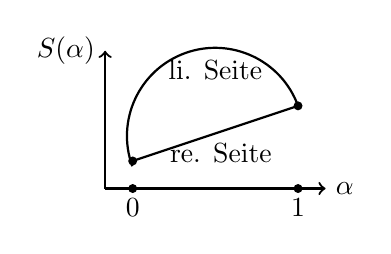
\begin{tikzpicture}[scale=0.7]
            \draw[->,thick](0,0) -- (4,0) node[anchor=west]{$\alpha$};
            \draw[->,thick](0,0) -- (0,2.5) node[anchor=east]{$S(\alpha)$};
            \filldraw[black] (0.5,0.5) circle (2pt);
            \filldraw[black] (3.5, 1.5) circle (2pt);
            \filldraw[black] (0.5,0) circle (2pt) node[anchor=north]{0};
            \filldraw[black] (3.5,0) circle (2pt) node[anchor=north]{1};
            \draw[-,thick](0.5,0.5) -- (3.5,1.5);
            \draw[-, thick](3.5,1.5) arc (20:200:1.6);
            \draw[] (2,2.5) node[anchor=north]{li. Seite};
            \draw[] (2.1,1) node[anchor=north]{re. Seite};
        \end{tikzpicture}
        \end{center}
        \item[] Bedeutung: Mischung von Verteilungen erhöht Entropie (Mischungsentropie) 
    \end{itemize}
\end{enumerate}
\end{prop}



\subsubsection{statistische Entropie eines quantenmechanischen Makrozustands}
\textbf{Falsch:} $\hat{\varrho} = \sum_n w_n \ket{\Psi_n}\bra{\Psi_n} \ \Rightarrow \ S(\hat{\varrho}) = -k\cdot\sum_n w_n \ln{w_n} $\\
\textbf{Problem:} Viele Kombinationen $\{w_n\, , \,\ket{\Psi_n}\}$ ergeben gleichen Dichteoperator $\hat{\rho} \ \Rightarrow \ S(\hat{\varrho})$ darf nur von $\hat{\varrho}$ abhängen und nicht von den verschiedenen $\{w_n\, ,\, \ket{\Psi_n}$.

\textbf{Richtig:} 
\begin{definition}{statistische Entropie eines qm Zustands}
    \begin{equation}
    S(\hat{\varrho}) = -k \cdot \trace (\hat{\varrho} \ln{\hat{\varrho}}) = -k \ \langle\ln{\hat{\varrho}}\rangle
    \end{equation}
\end{definition}

Wähle Eigenzustände von $\hat{\varrho}$ aus Basis für die Spur:
\begin{equation}
    \hat{\varrho} \ket{\varphi_n} = p_n \ket{\varphi_n}
\end{equation}


\begin{equation}
    \Rightarrow \ \ S(\hat{\rho}) = -k \cdot \sum_n \bra{\varphi_n} \hat{\varrho} \ln\hat{\varrho} \ket{\varphi_n} = -k \cdot \sum_n p_n \ln{p_n}
\end{equation}

\textbf{wichtig:} $p_n$ sind Eigenwerte zu $\hat{\varrho}$! 

\subsubsection*{Reiner Zustand:}
$\hat{\varrho}^2 = \hat{\varrho}$ anwenden auf $\ket{\varphi_n}$ (Eigenzustand von $\varrho$)

\begin{align}
    \Rightarrow \ \forall n: \ &&\hat{\varrho}^2 \ket{\varphi_n} = \hat{\varrho} \ket{\varphi_n}  \\
    \Rightarrow \ \forall n: \ &&p_n^2 \ket{\varphi_n} = p_n \ket{\varphi_n} \\
    \Rightarrow \ \forall n: \  &&p_n^2= p_n \\
    \Rightarrow \  \forall n: \  &&p_n = 0 \text{ oder } p_n = 1 \\
\end{align}
 \begin{equation}
   \Rightarrow \  \  S(\hat{\varrho}) = 0 , \text{ da volle Information}  
 \end{equation}
 
\subsubsection*{Gemischter Zustand:}
$\hat{\varrho}^2 \neq \varrho$
\begin{align}
    &\exists \ n:  \ &&p_n^2 = p_n\\
    \Rightarrow \ &\exists \ n:  \ &&0 < p_n < 1 \\
    \Rightarrow \ &S(\hat{\varrho}) > 0 \ &&\text{, d.h. Information fehlt!}
\end{align}
Maximale Entropie: \ \ Gleichverteilung $p_n = \frac{1}{M} \ \Rightarrow \ S = k \ln M$

\subsubsection{Statistische Entropie eines klassischen Makrozustands}

WS-Dichte $\varrho ( \Vec{q}, \Vec{p})$ im Phasenraum ist Funktion der kontinuierlichen Variablen $\Vec{q}, \Vec{p}$

$\Rightarrow$ keine diskreten WS $p_i \ \Rightarrow$ Problem

Betrachte Phasenraumzellen $\Gamma_i$ mit Volumina $\tau$ \\
$\Rightarrow$ diskrete WS $p_i$

\begin{equation}
    p_i = \int_{\Gamma_i} d\Vec{q} \, d\Vec{p}_i \ \varrho (\Vec{q}, \Vec{p}) \overset{(*)\text{\tiny{ $\varrho$ glatt}}}{\approx} \tau \varrho (\Vec{q}, \Vec{p}) \ \text{ für Punkt } (\Vec{q}, \Vec{p}) \in \Gamma_i
\end{equation}
(*) Wenn $\varrho$ glatt, dann ist es auf kleiner Umgebung von $(\Vec{q}_i,\Vec{p}_i)$ konstant und man $\varrho $ vor das Integral ziehen. (Hier wird angenommen, dass diese Bedingung immer erfüllt ist. Das ist sinnvoll, da $ h \sim 10^{-34}$ sehr kleine Größenordnung. \\
Bedingung ist beispielsweise bei multifraktalen WS-Verteilungen nicht erfüllt.)\\

$\Rightarrow$ statistische Entropie einer WS-Dichte im Phasenraum: \\
\begin{equation}
    S\bigl(\varrho(\Vec{q}, \Vec{p})\bigr) \approx -k \cdot\sum_i \tau \ \varrho(\Vec{q}_i,\Vec{p}_i)\ln \bigl(\tau \varrho (\Vec{q}_i, \Vec{p}_i)\bigr)
\end{equation}

\begin{definition}{Entropie}
    \begin{equation}
        S \bigl(\varrho ( \Vec{q},\Vec{p}) \bigr) = - k \ \int_\Gamma d\Vec{q} \, d\Vec{p} \ \varrho(\Vec{q},\Vec{p}) \ \ln{\bigl(\tau \ \varrho(\Vec{q},\Vec{p}\bigr)}
    \end{equation}
    
\end{definition}

\textbf{Probleme:}
\begin{itemize}
    \item[-] Abhängig von $ \tau$, divergiert für $\tau \rightarrow 0$
    \item[$\Rightarrow$] Lösung: Heisenbergsche Unschärferelation $\Delta q \Delta p \geq \frac{\hbar}{2}$
    \item[$\Rightarrow$] Elementarzelle $\tau \sim \hbar^f$ \ (f... Anzahl der Freiheitsgrade)
\end{itemize}

später: Planck-Zelle $\tau = h^f$

\begin{beispiel}{Beispiel: Gleichverteilung}
    Sei $\varrho=$ const. im Volumen $\Gamma$ des Phasenraums $\Rightarrow \ \varrho = \frac{1}{\Gamma}$ \\
    Zahl der Planck-Zellen: \ $M = \frac{\Gamma}{\tau} \ \Rightarrow \ \tau \varrho = \frac{\Gamma}{M} \frac{1}{\Gamma} = \frac{1}{M}$
    \begin{equation*}
        \Rightarrow \ S(\varrho = \text{ const. }) = -k \ \ln{\frac{1}{M}} \underbrace{\int_\Gamma d\Vec{q} \, d\Vec{p} \ \varrho(\Vec{q},\Vec{p})}_{=1} = k \ln M
    \end{equation*}

    \textbf{Bemerkung:} 
    \begin{itemize}
        \item[-] Entropie mit diskreten WS natürlich definiert
        \item[-] in klassischer Mechanik muss $\underbrace{\text{Planck-Zelle}}_{\text{sinnvoll, wegen Heisenberg Unschärfe}}$ eingeführt werden. (In qm ist das Konzept von Trajektorien bzw. Punkten im Phasenraum aufgrund der Unschärferelation nicht vorgesehen.)
    \end{itemize}
\end{beispiel}

\subsection{Gleichgewichtsensemble und Prinzip der maximalen Ensemble} \marginpar{VL 6}
Zustand eines Systems im themodynamischen Gleichgewicht $\Bigl( \frac{\partial \hat{\varrho}}{\partial t} = 0 \Bigr)$ charakterisiert durch:
\begin{itemize}
    \item Erhaltungsgrößen: Energie, Gesamtimpuls, Gesamtdrehimpuls, Teilchenzahl
    \item äußere Parameter: Volumen, Druck, Temperatur
\end{itemize}

System ist durch Wände begrenzt:
\begin{itemize}
    \item[$\Rightarrow$] Gesamtdrehimpuls und Gesamtimpuls nicht erhalten
    \item[$\Rightarrow$] Energie und Teilchenzahl möglich Erhaltungsgrößen
\end{itemize}

Die 3 wichtigsten Gleichgewichts-Ensemble sind: (\emph{$\rightarrow$ experimentell schwierig: Energie erhalten und Teilchenzahl nicht $\rightarrow$ 3 Möglichkeiten})

\begin{enumerate}
    \item \underline{Mikrokanonisches Ensemble:} \\
    isoliertes System:
    \begin{itemize}
        \item feste Energie $E$
        \item feste Teilchenzahl $N$
    \end{itemize}
    \item \underline{kanonisches Ensemble:} \\
    Austausch von Energie mit Umgebung $\Rightarrow$ Energie fluktuiert
    \begin{itemize}
        \item mittlere Energie $\langle E \rangle$ stellt sich ein; abhängig von Umgebung (insbesondere Temperatur)
        \item Teilchenzahl $N$ fest
    \end{itemize}
    \item \underline{Großkanonisches Ensemble}
    Austausch von Energie und Teilchen mit Umgebung
    \begin{itemize}
        \item[$\Rightarrow$] Energie und Teilchenzahl funktioniert
        \item mittlere Energie $\langle E \rangle$
        \item mittlere Teilchenzahl $\langle N \rangle$ stellt sich ein. Beides ist abhängig von der Umgebung
    \end{itemize}
\end{enumerate}

Welcher Dichteoperator $\hat{\varrho}$ beschreibt den Makrozustand zum jeweiligen Gleichgewichts-Ensemble?
\begin{equation*}
    \Longleftrightarrow
\end{equation*}
Was sind die Wahrscheinlichkeiten $p_n$ der Energie-Eigenzustände $E_n$?

\begin{prop}{Prinzip der maximalen Entropie (Jaynes, 1957)}
    Makrozustand im thermodynamischen Gleichgewicht wird mit dem Dichteoperator $\hat{\varrho}$ beschrieben, der die Entopie unter Einhaltung der Nebenbedingungen (z.B. mittlere Energie) \textbf{maximiert}.
\end{prop}

\underline{Bemerkung:}
\begin{itemize}
    \item Es wird nur die bekannte Information benutzt
    \item Jeder andere Dichteoperator $\hat{\varrho}$ mit kleinerer Entropie beinhaltet mehr Information über das System
\end{itemize}

\subsection{Mikrokanonisches Ensemble}\label{seq.Mikrokanonisches_ensemble}
Isoliertes System mit fester Energie $E$ und fester Teilchenzahl $N$.
\begin{center}
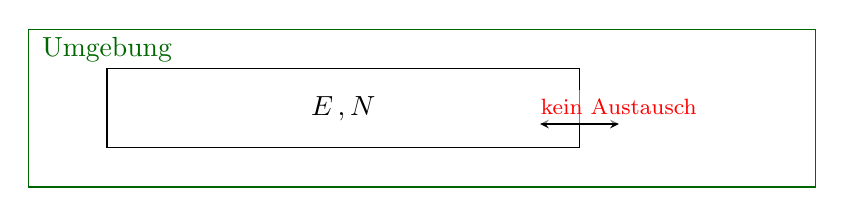
\begin{tikzpicture}
    \draw[green!40!black] (0,0)--(10,0)--(10,2)--(0,2)--(0,0);
    \draw (1,0.5)--(7,0.5)--(7,1.5)--(1,1.5)--(1,0.5);
    \draw[stealth-stealth] (6.5,0.8)--(7.5,0.8) node[above, red, fill=white,opacity=.5,text opacity=1] {\footnotesize{kein Austausch}};
    \draw (4,1) node {$E\, ,N$};
    \draw (1,1.75) node[green!40!black] {Umgebung};
\end{tikzpicture}
\end{center}

Teilchenzahl $N$ als diskrete Variable wird exakt angenommen; Energie $E$ ist kontinuierliche Variable
\begin{itemize}
    \item zu vorgegebener Energie $E$ gibt es i.A. keinen Mikrozustand mit $E_n = E$
    \item physikalische Messung ist mit Unsicherheit $\Delta E$ verbunden
    \item[$\Rightarrow$] Man betrachtet ein Energieintervall $[E-\Delta E,E]$ mit:
    \begin{enumerate}
        \item $\Delta E \ll E$
        \item $\Delta E$ groß genug, damit es viele Mikrozustände im Intervall gibt
        \item Vorhersagen sollten nicht von $\Delta E$ abhängen
    \end{enumerate}
\end{itemize}

Wie groß ist WS $p_n$ für Mikrozustand (=Energie-Eigenzustand) $\ket{\phi_n}$ mit $E_n \in [E-\Delta E,E]$?
\begin{itemize}
    \item[] Prinzip der maximalen Entropie mit Nebenbedingung: $\sum_n \ p_n = 1$
    \begin{equation}
        \stackrel{\equa{Geichverteilung}}{\Longrightarrow} \text{Gleichverteilung mit } p_n = const.
    \end{equation}
    \item[] (äquivalentes Postulat: alle Eigenzustände $\ket{\phi_n}$ eines isolierten Systems mit $E_n \in [E-\Delta E,E]$ haben gleiche Wahrscheinlichkeit. Es gibt keinen Grund, einen der Eigenzustände gegenüber anderen hervorzuheben.)
\end{itemize}

\paragraph{WS im mikrokanonischen Ensemble}
\begin{equation}
    p_n = \begin{cases}
        \frac{1}{M_{\Delta}(E)} \qquad \text{; falls } E_n \in [E-\Delta E,E] \\
        0 \qquad \text{; sonst}
    \end{cases}
\end{equation}
$M_{\Delta}(E)$ ist die Zahl der Zustände in $[E-\Delta E,E]$

\paragraph{Dichteoperator im mikrokanonischen Ensemble}
\begin{equation}
    \hat{\varrho} \ = \ \sum_n \ p_n \ \ket{\psi_n} \bra{\psi_n} \ = \ \frac{1}{M_{\Delta}(E)} \ \sum_{\substack{n \\ E_n \in [E-\Delta E,E]}} \ \ket{\psi_n} \bra{\psi_n}
\end{equation}
\begin{equation}
    \text{Test: } \trace(\hat{\varrho}) = \frac{1}{M_{\Delta}(E)} \ \sum_{\substack{n \\ E_n \in [E-\Delta E,E]}} \ \underbrace{\trace(\ket{\psi_n} \bra{\psi_n})}_{\braket{\psi_n}=1} \ = \ 1 \qquad \checkmark
\end{equation}

\paragraph{Mittelwerte im mikrokanonischen Ensemble}
\begin{equation}
    \langle \hat{A} \rangle = \trace(\hat{\varrho} \hat{A}) = \frac{1}{M_{\Delta}(E)} \ \sum_{\substack{n \\ E_n \in [E-\Delta E,E]}} \ \underbrace{\trace(\ket{\psi_n} \bra{\psi_n} \hat{A})}_{= \trace(\bra{\psi_n} \hat{A} \ket{\psi_n})}
\end{equation}
anschaulich: Mittelwert der Erwartungswerte

\paragraph{Dichteoperator im Limes $\Delta E \to 0$}
\begin{equation}
    \hat{\varrho} = \frac{\delta(E-H)}{\trace(\delta(E-H))}
\end{equation}

\paragraph{WS-Dichte im klassischen Phasenraum}
\begin{equation}
    \varrho(\Vec{q},\Vec{p}) = \frac{\delta(E-H(\Vec{q},\Vec{p}))}{\int d\Vec{q} \int d\Vec{p} \ \delta(E-H(\Vec{q},\Vec{p}))}
\end{equation}
$\delta$-Funktion auf Energieschale
\begin{center}
    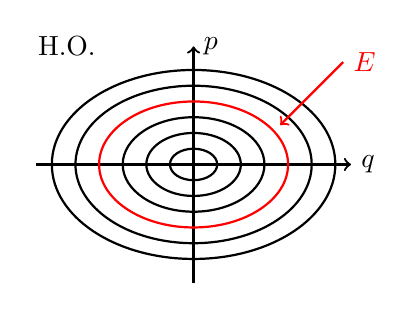
\begin{tikzpicture}
        \draw[->, thick] (-2,0) -- (2,0) node[anchor=west]{$q$};
        \draw[->, thick] (0,-1.5) -- (0,1.5) node[anchor=west]{$p$};
        \draw[] (-2.1, 1.5) node[anchor=west]{H.O.};
        \draw[thick] (0,0) ellipse (0.3 and 0.2);
        \draw[thick] (0,0) ellipse (0.6 and 0.4);
        \draw[thick] (0,0) ellipse (0.9 and 0.6);
        \draw[red, thick] (0,0) ellipse (1.2 and 0.8);
        \draw[thick] (0,0) ellipse (1.5 and 1.0);
        \draw[thick] (0,0) ellipse (1.8 and 1.2);
        \draw[<-, thick, red] (1.1,0.5) -- (1.9,1.3) node[anchor=west]{$E$};
    \end{tikzpicture}
\end{center}

\subsubsection{Zustandssumme, Zustandsdichte}
\emph{(ab jetzt: Mikrozustand = Energie-Eigenzustand = Zustand)}

\begin{center}

    \begin{tikzpicture}
    \draw[thick,->] (0,0) -- (5,0) node[anchor=north west] {$E$};
\draw[thick,->] (0,0) -- (0,3.5) node[anchor=south east] {$M_{\Delta}(E)$};
    \foreach \x in {0,1,2,3,4}
   \draw (\x cm,1pt) -- (\x cm,-1pt) node[anchor=north] {};
    \foreach \y in {0,1,2,3}
    \draw (1pt,\y cm) -- (-1pt,\y cm) node[anchor=east] {$\y$};
    \draw[red] (0,1)--(1.2,1)--(1.2,2)--(2.8,2)--(2.8,3)--(4.4,3);
    \draw (1.2,1pt)-- (1.2,-1pt)node[anchor=north] {$E_1$};
    \draw (2.8,1pt)-- (2.8,-1pt)node[anchor=north] {$E_2$};
    \draw (4.4,1pt)-- (4.4,-1pt)node[anchor=north] {$E_3$};
    \end{tikzpicture}

    \begin{tikzpicture}
    \draw[thick,->] (0,0) -- (5,0) node[anchor=north west] {$E$};
\draw[thick,->] (0,0) -- (0,3.5) node[anchor=south east] {$d(E)$};
    \foreach \x in {0,1,2,3,4}
   \draw (\x cm,1pt) -- (\x cm,-1pt) node[anchor=north] {};
    \foreach \y in {0,1,2,3}
    \draw (1pt,\y cm) -- (-1pt,\y cm) node[anchor=east] {$\y$};
    \draw (1.2,1pt)-- (1.2,-1pt)node[anchor=north] {$E_1$};
    \draw (2.8,1pt)-- (2.8,-1pt)node[anchor=north] {$E_2$};
    \draw (4.4,1pt)-- (4.4,-1pt)node[anchor=north] {$E_3$};
    \draw[red,->] (1.2,0)-- (1.2,3.5)node[anchor=north] {};
    \draw[red,->] (2.8,0)-- (2.8,3.5)node[anchor=north] {};
    \draw[red,->] (4.4,0)-- (4.4,3.5)node[anchor=north] {};
    \draw[-,thick,red] (0,0) -- (4.99,0);
    \end{tikzpicture}
\end{center}

\begin{definition}{Mikrokanonische Zustandssumme}
    \begin{align}
        Z &\coloneqq M(E) = \sum_n \ \Theta(E-E_n) \qquad \text{Anzahl der Zustände mit } E_n < E \\
        z &\coloneqq M_{\Delta}(E) = \sum_n \ \Theta(E - E_n) \Theta(E_n-(E-\Delta E)) \qquad \text{Anzahl mit } E_n \in [E- \Delta E, E]
    \end{align}
\end{definition}

\underline{Bemerkung:}
\begin{itemize}
    \item beide Definitionen unterscheiden sich bei großer Teilchenzahl nicht
    \begin{itemize}
        \item[Bsp.:] Volumen der Kugel vs Volumen einer Kugelschale an der Oberfläche
        \item[] in 3D vs in $6\cdot 10^{23}$D
    \end{itemize}
    \item kanonische und großkanonische Zustandssumme haben andere Definitionen
\end{itemize}

\begin{definition}{Zustandsdichte}
    \begin{equation}
        d(E):= \frac{d \ M(E)}{d \ E} = \sum_n \delta(E-E_n)
    \end{equation}
\end{definition}

\begin{beispiel}{Rechenbeispiel}
    \begin{equation}
        \int_{-\infty}^E dE^\prime \ d(E^\prime) = \int_{-\infty}^E dE^\prime \ \sum_n \delta(E_n -E^\prime)= \sum_n\ \int_{-\infty}^E dE^\prime \ \delta(E_n -E^\prime) = \sum_{\overset{n}{E_n<E}} 1 = M(E)
    \end{equation}
\end{beispiel}

\marginpar{VL 7}
\subsubsection{Ideales Gas}\label{seq.ideales Gas}
\begin{itemize}
    \item $N$ Teilchen, Masse $m$, Volumen $V$
    \item keine WW, punktförmig, keine innere Struktur (einatomig)
    \item Hamilton-Fkt., Hamilton-Operator
    \begin{equation}
        H = \sum_{j=1}^N \frac{\Vec{p_j}^2}{2m} \qquad \Vec{q} \in V
    \end{equation}
    \item[Ziele]:
    \begin{itemize}
        \item Bestimme Zahl der Zustände qm und klassisch
        \item Vergleich $\Rightarrow$ Größe der Planck-Zelle
    \end{itemize}
\end{itemize}

\paragraph{Quantenmechanisches ideales Gas}
Energie-Eigenzustände:
\begin{itemize}
    \item 1D, N = 1: Quantenzahl n = 1,2,...
    \begin{align}
        \varphi_n(x) &= A_1 \cdot sin\left(\frac{\pi}{L} n x \right) \\
        E_n &= \frac{\hbar^2}{2m} \left(\frac{\pi}{L} n \right)^2 = \frac{h^2}{8mL^2} n^2
    \end{align}
    
    \begin{center}
    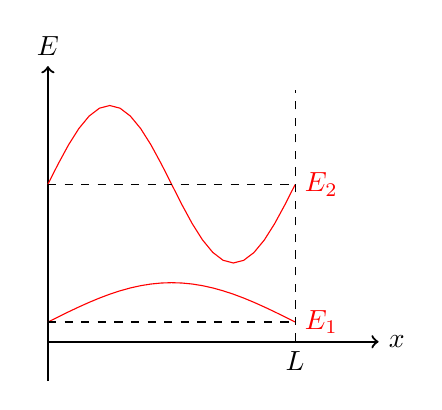
\begin{tikzpicture}[domain=0:3.14]
  \draw[->, thick] (-0.01,0) -- (4.2,0) node[right] {$x$};
  \draw[->, thick] (0,-0.5) -- (0,3.5) node[above] {$E$};
  \draw[color=red]   plot (\x,{0.5*(sin(\x r)+0.5)})    node[right] {$E_1$};
  \draw[color=red] plot (\x,{sin(\x*2 r)+2}) node[right] {$E_2$};
  \draw[dashed] (3.14,0) --(3.14,3.2);
  \draw[dashed] (0,0.25) --(3.14,0.25);
  \draw[dashed] (0,2) --(3.14,2);
  \node[below] at (3.14,0) {$L$};
\end{tikzpicture}
\end{center}

    \item 3D, N=1: Quantenzahlen $n_x,n_y,n_z$ ($L_x=L_y=L_z=L$)
    \begin{align}
        \varphi_{n_x,n_y,n_z}(\Vec{r}) &= A_3 \cdot sin\left(\frac{\pi}{L} n_x x \right)  sin\left(\frac{\pi}{L} n_y y \right)  sin\left(\frac{\pi}{L} n_z z \right) \\
        E_{n_x,n_y,n_z} &= \frac{h^2}{8mL^2} \underbrace{(n_x^2 + n_y^2 +n_z^2)}_{\text{3D-Gitter mit Abstand 1}}
    \end{align}
    
    \begin{figure*}
    \centering
    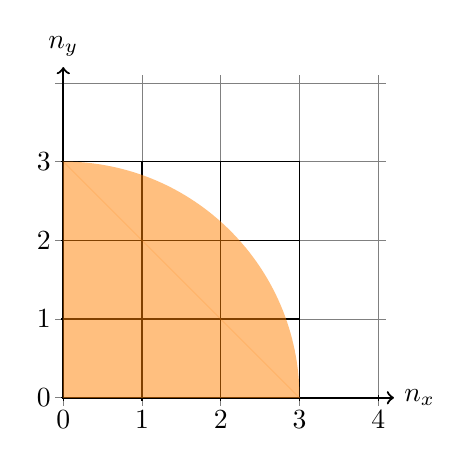
\begin{tikzpicture}
     \draw[very thin,color=gray] (-0.1,-0.1) grid (4.1,4.1);
     \foreach \y in {0,1,2,3}
    \draw (1pt,\y cm) -- (-1pt,\y cm) node[anchor=east] {$\y$};
    \foreach \x in {0,1,2,3,4}
   \draw (\x cm,1pt) -- (\x cm,-1pt) node[anchor=north] {$\x$};
    \draw[->, thick] (-0.01,0) -- (4.2,0) node[right] {$n_x$};
  \draw[->, thick] (0,-0.01) -- (0,4.2) node[above] {$n_y$};
   \draw (0.5,0.5) node[minimum height=1cm,minimum width=1cm,draw] {};
   \draw (0.5,1.5) node[minimum height=1cm,minimum width=1cm,draw] {};
   \draw (0.5,2.5) node[minimum height=1cm,minimum width=1cm,draw, fill=white] {};
   \draw (2.5,0.5) node[minimum height=1cm,minimum width=1cm,draw, fill=white] {};
   \draw (1.5,0.5) node[minimum height=1cm,minimum width=1cm,draw, fill=white] {};
   \draw (1.5,1.5) node[minimum height=1cm,minimum width=1cm,draw, fill=white] {};
   \draw (1.5,2.5) node[minimum height=1cm,minimum width=1cm,draw, fill=white] {};
   \draw (2.5,1.5) node[minimum height=1cm,minimum width=1cm,draw, fill=white] {};
   \draw (2.5,2.5) node[minimum height=1cm,minimum width=1cm,draw, fill=white] {};
   \draw[thick, red, fill=orange,opacity=.5, draw=none] (3,0) arc (0:90:3);
   \filldraw[fill=orange, opacity =.5, draw=orange, draw opacity = .1] (0,0) -- (0,3) -- (3,0);
    \end{tikzpicture}
    \caption{Abzählung der Zustände in 2D}
\end{figure*}

    \item 3D, N: Quantenzahlen $n_{1x},n_{1y},n_{1z},n_{2x},\dots, n_{Nz}$
    \begin{align}
        E_{n_{1x},\dots,n_{Nz}} = \frac{h^2}{8mL^2} &\underbrace{(n_{1x}^2 + \dots + n_{Nz})}_{(\text{Abstand vom Ursprung})^2} \\ 
        &_\text{in 3N-dim. Gitter mit Gitterabstand 1}
    \end{align}
\end{itemize}

Zahl der Zustände mit Energie kleiner $E$:
\begin{equation}
    M(E) = \frac{V_{3N}\left(\sqrt{\frac{8mL^2 E}{h^2}}\right)}{\underbrace{1^{3N}}_{\text{Einheitszelle}}} \cdot \underbrace{\left( \frac{1}{2}\right)^{3N}}_{\text{\glqq Viertelkreis \grqq}}
\end{equation}

Volumen der f-dim. Kugel mit Radius $R$:
\begin{equation}
    V_f(R) = c_f \cdot R^f \qquad c_f = \frac{\pi^{f/2}}{\frac{f}{2}\Gamma(\frac{f}{2})}
\end{equation}
\begin{center}
\fcolorbox{red}{white}{
\begin{equation}
    \hspace{2cm} M(E) \quad = \quad c_{3N} \left( \frac{8 m L^2 E}{h^2}\right)^{\frac{3N}{2}} \frac{1}{2^{3N}} \quad  = \quad c_{3N} \frac{1}{h^{3N}} (2m)^{\frac{3N}{2}} V^N E^{\frac{3N}{2}} \hspace{2cm}
\end{equation}
}
\end{center}
\textbf{Bemerkung:}
\begin{enumerate}
    \item Ununterscheidbarkeit nicht berücksichtigt $\Rightarrow$ Formel bei Diskussion Quantengase korrigiert
    \begin{itemize}
        \item unterschiedliche Ausdrücke für Fermionen und Bosonen
        \item Grenzfall: WS Besetzung eines Zustands $\ll 1$ (Maxwell-Boltzmann-Näherung)
        \item[$\Rightarrow$] Korrekturfaktor $\frac{1}{N!}$ 
    \end{itemize}
    \item Extrem starke Zunahme mit $E$
    \item Vergleiche beide Definitionen der mikrokanonischen Zustandssumme $Z = M(E)$ und $y = M_\Delta (E) = M(E) -M(E_\Delta)$:
    \begin{align}
        \frac{z}{Z} = \frac{M_\Delta(E)}{M(E)} = 1 - \frac{M(E-\Delta)}{M(E)} = 1 -\frac{(E-\Delta)^{3N/2}}{E^{3N/2}} = 1- \Bigl( 1- \frac{\Delta}{E}\Bigr)^{3N/2}  \\
        = 1- e^{\ln(^-\frac{\Delta}{E})^{3N/2}} = \underbrace{1- e^{\frac{3N}{2} \ \ln{(1-\frac{\Delta}{E})}}}_{\text{Taylorentwicklung: } \ln (1-\frac{\Delta}{E}) \approx -\frac{\Delta}{E}} \overset{\Delta \ll E}{=} 1- e^{\frac{3N}{2} \frac{\Delta}{E}}
    \end{align}
\end{enumerate}

Fallunterscheidung:
\begin{itemize}
    \item[-] \underline{$\frac{N \Delta}{E} \ll 1$:} $\Leftrightarrow \ \ \frac{\Delta}{E} \ll \frac{1}{N} \ \ \Leftrightarrow \ \ \Delta \ll \frac{E}{N}$ (mittlere Energie pro Teilchen): \\
    \begin{equation}
        \frac{M_\Delta(E)}{M(E)} \approx 1- \Bigl( 1- \frac{3N}{2} \frac{\Delta}{E} \Bigr)= \frac{3N}{2} \frac{\Delta}{E}
    \end{equation}
    \item[-] \underline{$1 \ll \frac{N \Delta}{E}:$} $\Leftrightarrow \ \ \frac{1}{N} \ll \frac{\Delta}{E} \ll 1 \ \ \Leftrightarrow \ \ \frac{E}{N} \ll \Delta \ll E$
    \begin{equation}
        \frac{M_\Delta(E)}{M(E)} \approx 1
    \end{equation}
    unabhängig von $\Delta$
    \item[-] \underline{$\frac{N\Delta}{E} \approx 1$:} keine Näherung möglich! 
    \item[$\rightarrow$] $N = 10^{23} \ \ \Rightarrow$ Bereich riesig: Messfehler ist in diesem Bereich
     \item[$\Rightarrow$] Physikalisch relevanter Bereich
      \item[$\rightarrow$] Zahl der Zustände $M_\Delta(E) \approx M(E)$ (mikrokanonische Zustandssumme $z \approx Z$)
       \item[$\rightarrow$]mikrokanonisches Ensemble berücksichtigt fast alle Zustände $E_n < E$
\end{itemize}

\paragraph{klassisches ideales Gas}
\begin{align}
    M(E) &= \frac{\text{\footnotesize{erlaubtes Phasenvolumen}}}{\text{\footnotesize{Volumen der Planck-Zelle}}} = \frac{\int_{H (\Vec{q},\Vec{p}) < E} d\Vec{q}\, d\Vec{p}}{\tau} \underbrace{\frac{1}{N!}}_{\text{Ununterscheidbarkeit- Gibbs-Paradoxon}} \\
    &= \frac{1}{N! \tau} \int d\Vec{q} \, d\Vec{p} \ \Theta\bigl(E-H(\Vec{q}, \Vec{p})\bigr) \\
    &= \frac{1}{N! \tau} \underbrace{\int_0^L dq_1 \dots \int_0^L dq_{3N}}_{L^{3N}= V^N} \underbrace{\int_{-\infty}^\infty dp_1 \dots \int_{-\infty}^\infty dp_{3N} \ \Theta\bigl( E- \sum_{i=1}^{3N} \frac{p_i^2}{2m}\bigr)}_{V_{3N}\bigl(\sqrt{2mE}\bigr) = c_{3N} \, (2mE)^{\frac{3N}{2}}}\\
    &=c_{3N} \, \frac{1}{N! \, \tau} \, (2m)^{\frac{3N}{2}} \, V^N \, E^\frac{3N}{2}
\end{align}
Vergleich klassische und quantenmechanische Rechnung für dieses Bsp.:
\begin{center}
    \fcolorbox{red}{white}{$\tau = h^{3N}$}
\end{center}
 ist Volumen der Planck-Zelle

 \subsection{kanonisches Ensemble}\label{sec.Kanonisches Ensemble} \marginpar{VL 8}
 konstante Teilchenzahl $N$; Energieaustausch mit Umgebung.
 $\Rightarrow$mittlere Energie $\langle E\rangle$ stellt sich ein.

 \begin{center}
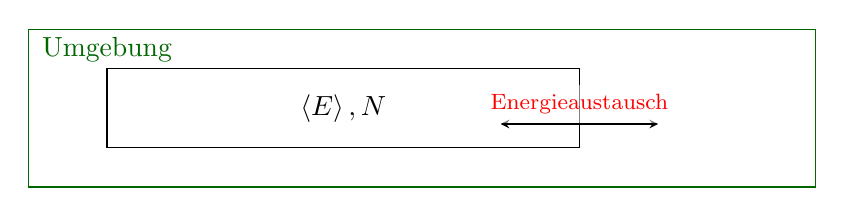
\begin{tikzpicture}
    \draw[green!40!black] (0,0)--(10,0)--(10,2)--(0,2)--(0,0);
    \draw (1,0.5)--(7,0.5)--(7,1.5)--(1,1.5)--(1,0.5);
    \draw[stealth-stealth] (6,0.8)--(8,0.8) node[above,midway, red, fill=white,opacity=.5,text opacity=1] {\footnotesize{Energieaustausch}};
    \draw (4,1) node {$\langle E\rangle \, ,N$};
    \draw (1,1.75) node[green!40!black] {Umgebung};
\end{tikzpicture}
\end{center}

\begin{itemize}
    \item[]Welche Dichteopeator $\varrho$ beschreibt den Mikrozustand?\tikzmark{start}
    \item[] Wie groß ist die WS $p_n$ für Eigenstustand $\ket{\varphi_n}$ Eigenenergie $E_n$ ?\tikzmark{end}
\end{itemize}

 
 \begin{tikzpicture}[remember picture,overlay]
    \draw[decorate,decoration={calligraphic brace}]
        ([yshift=10pt,xshift=10pt]{{pic cs:end}|-{pic cs:start}}) --
        node[xshift=5pt,anchor=west, text width=4cm] {identisch im \\ thermodynamischen Gleichgewicht}
        ([xshift=10pt]{pic cs:end})
;
\end{tikzpicture}

\subsubsection{Maximierung Entropie}

Entropie: 
\begin{equation}
    S=-k \trace\left(\varrho \ln \varrho\right)
\end{equation}
\begin{itemize}
    \item Variation von $\varrho$ unter Nebenbedingung
    \begin{equation}
        \trace(\varrho) =1
    \end{equation}
    \item Weitere Nebenbedingung
    \begin{equation}
        \trace(\varrho A_i) =\langle A_i \rangle
    \end{equation}
    \item[$\rightarrow$] kanonisches Ensemble ($i=1)$:  
    \begin{align}
        A_1 &=H & \langle A_1\rangle&=\langle H\rangle=\langle E\rangle
    \end{align}
    \item[$\rightarrow$] großkanonisches Ensemble ($i=2$):
    \begin{align}
        A_1 &=H & \langle A_1\rangle&=\langle H\rangle=\langle E\rangle\\
        A_2 &= \hat{N} \text{ Teilchenzahl}& \langle A_2\rangle&= \langle N\rangle \text{ mittlere Teilchenzahl}
    \end{align}
\end{itemize}

Nutze Methode der Lagrange-Multiplikatoren \ref{lagrange}\\
$\Rightarrow$ Maximiere:
\begin{equation}
    \Tilde{S} \left(\varrho, \lambda, ,\ \{\lambda_i\}\right) = -k \color{black!30!white}\Bigl( \color{black} \trace \left( \varrho \ln\varrho \right) +\lambda\left( \trace \varrho -1\right) + \sum_i \lambda_i \left( \trace(\varrho A_i) -\langle A_i\rangle \right)  \color{black!30!white}\Bigr) \color{black}
\end{equation}
(Die grauen klammern werden einfach eingefügt. Sie verändern nur die Lagrange-Multiplikatoren. Die Rechnung wird aber erleichtert)

\begin{enumerate}
    \item[0. Schritt] Ableitung nach $\lambda, \, \{\lambda_i\}$ ergibt Nebenbedingungen
    \item[1. Schritt] Suche stationären Punkt $\delta\Tilde{S} =0$ unter Nebenbedingung $\delta\varrho$:
    \begin{equation}
        \delta\Tilde{S} = -k \trace \Bigl( \delta \varrho  \underbrace{(\ln \varrho +1 + \lambda+\sum_i \lambda_i A_i)}_{\stackrel{!}{=}0} \Bigr)
    \end{equation}
    $\Rightarrow$ stationäre Lösung:
    \begin{equation}
        \varrho= e^{-1-\lambda -\sum_i \lambda_i A_i} =: \frac{1}{Z} e^{-\sum_i \lambda_i A_i}
    \end{equation}
    \item[2. Schritt] Entropie der stationären Lösung:
    \begin{align}
        S(\varrho)&= -k \trace(\varrho \ln \varrho) =-k \trace\left( \varrho( -\ln(Z) - \sum_i \lambda_i A_i )\right) \\
        &=k \ln(Z) \underbrace{\trace \varrho}_{=1} +k \sum_i \lambda_i \underbrace{\trace(\varrho A_i)}_{= \langle A_i\rangle}
    \end{align}
    \begin{equation}
      \fcolorbox{red}{white}{$S(\varrho) =k \ln (Z) + k \sum_i \lambda_i \ \langle A_I\rangle$}
    \end{equation} \color{black!50!white}
    \item[3. Schritt] zeige, dass $S$ maximal ist. -Wird hier nicht gezeigt. Man nutze $S(\Tilde{\varrho } ) \leq -k \trace(\Tilde{\varrho} \ln \varrho)$. Der Beweis verbleibt als Übung für die Lesenden.
\end{enumerate}
\color{black}

\textbf{Zusammenfassung}

\begin{definition}{Boltzmann-Gibbs-Verteilung}
    \begin{equation}
        \hat{\varrho} = \frac{1}{Z} \ e^{-\sum_i \lambda_i A_i }
    \end{equation}
\end{definition}

\begin{definition}{Zustandssumme}
    $\trace\varrho=1 \ \Rightarrow$
    \begin{equation}
        Z\left( \{ \lambda_i\}\right) = \trace\left( e^{-\sum_i \lambda_i A_i}\right)
    \end{equation}
\end{definition}

 \begin{definition}{Entropie}
     \begin{equation}
         S(\varrho) =k \ln (Z) + k \sum_i \lambda_i \ \langle A_i\rangle
     \end{equation}
 \end{definition}

\subsubsection{kanonischer Dichteoperator, Kanonische Zustandssumme}

kanonisches Ensemble: \hspace{2cm} $A_1 = H \ \ \lambda\rightarrow\beta$ \hspace{2cm} (später: $\beta=\frac{1}{k_BT}$)


\begin{align}
    \hat{\varrho} &= \frac{1}{Z} \ e^{-\beta H} \\
    Z(\beta)&= \trace \left( e^{-\beta \hat{H}} \right) \hspace{2cm} \text{kanonische Zustandssumme} \\
    S(\hat{\varrho}) &= k \ln (Z) + k \beta \langle E \rangle 
\end{align}

In der Basis der Energie-Eigenzustände $\ket{\varphi_n}:$
\begin{equation}
    p_n = \bra{\varphi_n}\hat{\varrho} \ket{\varphi_n} = \frac{1}{Z} \bra{\varphi_n} \underbrace{e^{-\beta \hat{H}}\ket{\varphi_n}}_{e^{-\beta E_n \ket{\varphi_n}}} = \frac{1}{Z} e^{-\beta E_n}
\end{equation}

\begin{equation}
    \fcolorbox{red}{white}{\hspace{2cm} $p_n = \frac{1}{Z} e^{-\beta E_n} \hspace{1cm} \xRightarrow[\sum_n p_n =1]{} \hspace{1cm} Z(\beta) = \sum_n e^{-\beta E_n}$ \hspace{2cm}}
\end{equation}

Erwartungswert im Gleichgewicht:
\begin{equation}
    \langle E\rangle = \trace (\varrho H ) = \sum_n \bra{\varphi_n} \underbrace{\varrho}_{\varrho= \sum_i p_i \ket{\varphi_i}\bra{\varphi_i}}H\ket{\varphi_n} =\sum_n p_n E_n
\end{equation}

\paragraph{Bemerkung}
\begin{itemize}
    \item Zustände mit gleicher Energie $E_n$ haben gleiche WS ($\widehat{=}$ mikrokaninisch.)
    \item alle Zustände (mit bel. Energie) haben WS > 0.
    \item $\sum_n$ ist Summe über Zustände (und nicht Energie $E_n$; Entartung!)
\end{itemize}

\paragraph{Allgemeine Bemerkung zu Boltzmann-Gibbs-Verteilung:}
\begin{enumerate}
    \item Erwarungswerte $\langle A_i\rangle$ aus Zustandssumme $Z\left( \{\lambda_i \}\right)$
    \begin{align}
        \langle A_i \rangle &= \trace (\varrho A_i ) = \trace \left( \frac{1}{Z} \, e^{-\sum_j \lambda_j A_j } A_i \right) = -\frac{1}{Z} \frac{\partial}{\partial \lambda_i} \underbrace{\trace\left( e^{-\sum_j \lambda_j A_j}\right)}_{Z} \\
        &= - \frac{\partial}{\partial \lambda_i} \ln \left( Z(\{\lambda_i\}\right)
    \end{align}
    \item Die Lagrange-Multiplikatoren $\lambda_i$ haben makroskopisch physikalische Interpretation $\rightarrow$ Umgebung
    \item Abhängigkeit der Entropie von Erwartungswerten
    \begin{align}
        \frac{\partial S \left( \langle A_i \rangle, \langle A_2 \rangle ,\dots \right)}{\partial \langle A_i \rangle} &= k \lambda_i & \frac{\partial S \left( \langle E \rangle\right)}{\partial \langle E \rangle}&= k \beta = \frac{1}{\beta}
    \end{align}
\end{enumerate}

\subsubsection{klassisches kanonisches Ensemble}
$f$ Freiheitsgrade $q_1, ... , q_f, \, p_1, ... , p_f, \, H(\Vec{q},\Vec{p})$

\begin{align}
    &\textbf{qm} &\longrightarrow \hspace{1cm} &\textbf{klass}\\
    \varrho &= \frac{1}{Z(\beta)} e^{-\beta H} &\longrightarrow \hspace{1cm}& \varrho(\Vec{q},\Vec{p}) = \frac{1}{Z(\beta)} e^{-\beta H(\Vec{q},\Vec{p})} \\
    \trace\varrho &=1 &\longrightarrow\hspace{1cm} &  \frac{1}{N!} \frac{1}{h^f} \int d\Vec{q} \, d\Vec{p} \ \varrho(\Vec{q}, \Vec{p}) =1 \\
    Z(\beta)&= \trace (e^{-\beta H}) &\longrightarrow\hspace{1cm} & Z(\beta) = \frac{1}{N!} \frac{1}{h^f} \int d\Vec{q} \, d\Vec{p} \ e^{- \beta H(\Vec{q},\Vec{p})} \\
    \langle A \rangle &= \trace(\varrho A) & \longrightarrow \hspace{1cm}& \langle A(\Vec{q}, \Vec{p}) \rangle = \frac{\int d\Vec{q} \, d\Vec{p} \ A(\Vec{q}, \Vec{p}) \ e^{- \beta H(\Vec{q},\Vec{p})} }{\int d\Vec{q} \, d\Vec{p} \ e^{- \beta H(\Vec{q},\Vec{p})}} \\
    %\frac{\frac{1}{N! \, h^f} \int d\Vec{q} \, d\Vec{p} \ e^{- \beta H(\Vec{q},\Vec{p})} }{\int d\Vec{q} \, d\Vec{p} \ e^{- \beta H(\Vec{q},\Vec{p})}} \\
    \text{speziell: } \langle H \rangle &= - \frac{d}{d \beta} \ln(Z(\beta)) & \longrightarrow \hspace{1cm}&\langle H \rangle = - \frac{d}{d \beta} \ln(Z(\beta)) 
\end{align}
Die Wahrscheinlichkeit für eine einzelne Koordinate $q_f \in [q_f, q_f + dq_f]$ ergibt sich zu:
\begin{align}
    w(q_f) \cdot dq_f &= \frac{1}{N! \, h^f} \int d\Vec{p} \ \int dq_1^{\prime} \dots \int dq_{f-1}^{\prime} \ dq_f^{\prime} \, \varrho(\Vec{q}^{\prime}, \Vec{p}) \\
    &= \frac{\int d\Vec{p} \ \int dq_1 \dots \int dq_{f-1} \ dq_f^{\prime} \, e^{- \beta \, H(\Vec{q}^{\prime}, \Vec{p})}}{\int d\Vec{p} \ \int dq_1^{\prime} \dots \int dq_{f-1}^{\prime} \ \int dq_f^{\prime} \, e^{- \beta \, H(\Vec{q}^{\prime}, \Vec{p})}}
\end{align}



\subsubsection{Gleichverteilungssatz} \marginpar{VL 9}
\emph{klassisch:} Sei in $H(\Vec{q},\Vec{p})$ ein quadratischer Term in $p_m$
\begin{align}
    H(\Vec{q},\Vec{p}) &= a \, p_m^2 + b \\
    \text{mit } a &= a(p_1, \dots, p_{m-1}, p_{m+1}, \dots, p_f,q_1,\dots, q_f) > 0 \\
    b &= b(p_1, \dots, p_{m-1}, p_{m+1}, \dots, p_f,q_1,\dots, q_f)
\end{align}
\emph{kanonisches Ensemble:}
\begin{align}
    \langle a \, p_m^2 \rangle &= \frac{\int d\Vec{q} \ \int d\Vec{p} \ a \, p_m^2 \, e^{-\beta(a p_m^2+b)}}{\int d\Vec{q} \ \int d\Vec{p} \ e^{-\beta(a p_m^2+b)}} \\
    &= \frac{\int d\Vec{q} \ \int dp_1 \dots \int dp_{m-1} \ \int dp_{m+1} \dots \int dp_f}{\int d\Vec{q} \ \int d\Vec{p} \ e^{-\beta(a p_m^2+b)}} \underbrace{\int_{\infty}^{\infty} dp_m \ p_m \ a \, p_m e^{-\beta(a p_m^2+b)}}
\end{align}
\begin{equation}
    \hspace{5cm} \stackrel{p.I.}{=} \underbrace{p_m \frac{e^{-\beta(a p_m^2 + b)}}{- 2 \beta}\Big|_{-\infty}^{\infty}}_{= 0} - \int_{-\infty}^{\infty} dp_m 1 \cdot \frac{e^{-\beta(a p_m^2 + b)}}{- 2 \beta}
\end{equation}
\begin{align}
   &= \frac{\int d\Vec{q} \ \int dp_1 \dots \int dp_{m-1} \ \int dp_{m+1} \dots \int dp_f}{\int d\Vec{q} \ \int d\Vec{p} \ e^{-\beta(a p_m^2+b)}} \frac{1}{2 \beta} \int_{-\infty}^{\infty} dp_m e^{-\beta(a p_m^2 + b)} \\
   &= \frac{1}{2 \beta} \color{black!50!white} = \frac{1}{2} k T \color{black} \rightarrow \text{Ergebnis unabhängig von a(\dots) und b(\dots)}
\end{align}

$\longrightarrow$ analog quaratischer Term in $q_m: \ H(\Vec{q},\Vec{p}) = a^{\prime} q_m^2 + b^{\prime}$
\begin{equation}
    \langle a^{\prime} q_m^2 \rangle = \frac{1}{2} k T
\end{equation}

\begin{definition}{Gleichverteilungssatz}
    Jeder unabhängige quadratische Term in $H(\Vec{q},\Vec{p})$ besitz den Erwartungswert $\frac{1}{2} k T$.
\end{definition}

\begin{beispiel}{Beispiel}
    \begin{itemize}
        \item 1D harmonischer Oszillator:
        \begin{align}
            H &= \frac{p^2}{2m} + \frac{1}{2} m \omega^2 q^2 \\
            &\Rightarrow \langle E \rangle = \langle E_{kin} \rangle + \langle E_{pot} \rangle = k T
        \end{align}
        \item 3D freies Teilchen:
        \begin{align}
            H &= \frac{p_x^2 + p_y^2 + p_z^2}{2 m} \\
            &\Rightarrow \langle E \rangle = \frac{3}{2} k T
        \end{align}
    \end{itemize}
\end{beispiel}



\subsubsection{Maxwellsche Geschwindigkeitsverteilung}
klassisches Gas im Potential $V(\Vec{p}).$\\

Betrachte 1 Teilchen im Wärmebad der anderen Teilchen (andere Teilchen $\widehat{=}$ Umgebung)\footnote{Frage aus Plenum: Ist diese Annahme, dass wir die anderen Teilchen als Umgebung betrachten sinnvoll? \\
Antwort:Ja. Das betrachtete Teilchen tauscht durch Stöße Energie mit den anderen Teilchen aus ($\widehat{=}$ Energieaustausch mit Umgebung.) Außerdem gilt globaler Energie- und Impulserhalt.\\
Das kanonische Ensemble kann angenommen werden, wenn sich die Umgebung nicht ändert. D.h. man muss warten, bis sich eine mittlere Energie $\langle E\rangle$ einstellt und sich die Umgebung damit zeitlich (statistisch) nicht mehr ändert.}

\begin{align}
    H(\Vec{q},\Vec{p}) &= \frac{\Vec{p}^2}{2m} + V(\Vec{q}) \\
    \varrho(\Vec{q},\Vec{p}) &= \frac{1}{Z} e^{- \beta H(\Vec{q},\Vec{p})} \propto e^{- \beta \left(\frac{\Vec{p}^2}{2m} + V(\Vec{q})\right)}
\end{align}

Impulsverteilung in einer Dimension:
\begin{equation}
    P(p_x) \propto e^{- \beta \frac{p_x^2}{2m}}
\end{equation}

\begin{center}
\begin{tikzpicture}
\begin{axis}[
    axis lines = left,
    xlabel = \(p_x\),
    ylabel = {\(P(p_x)\)},
     xticklabels={},
    yticklabels={}
]

\addplot [
    domain=-10:10, 
    samples=100, 
    color=red,
    line width=pt
]
{exp{-(0.3*x)^2}};
\end{axis}

\draw[<->] (2.35,2.4)--(4.5,2.4) node[above, midway] {$\sqrt{\frac{\beta}{m}}$};
\end{tikzpicture}   
\end{center}

Verteilung Betrag des Impulses: $p := \sqrt{\Vec{p}\cdot \Vec{p}}$
\begin{equation}
    P(p) \propto p^2 e^{-\beta \frac{p^2}{2m}}
\end{equation}

\begin{center}
    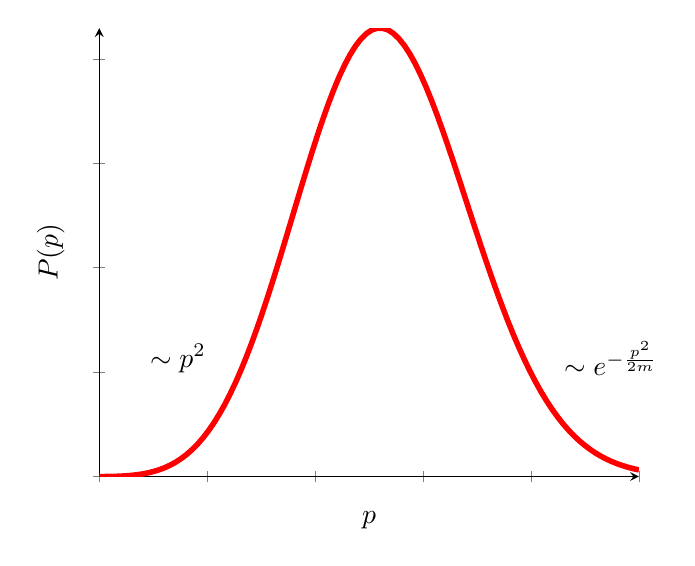
\begin{tikzpicture}
\begin{axis}[
    axis lines = left,
    xlabel = \(p\),
    ylabel = {\(P(p)\)},
     xticklabels={},
    yticklabels={}
]

\addplot [
    domain=0:10, 
    samples=100, 
    color=red,
    line width=2pt
]
{0.1*(x^2*exp{-(0.4*(x-4))^2})};

\end{axis}
\node[]at (1,1.5){$\sim p^2$};
\node[]at (6.5,1.5){$\sim e^{-\frac{p^2}{2m}}$};
\end{tikzpicture}
\end{center}



\begin{beispiel}{Bsp. in Vorlesung: Dynamische Animation mit 50 Teilchen im 2D-Billiard}
Zu Beginn haben alle Teilchen den gleichen Geschwindigkeitsbetrag.
    \begin{enumerate}
        \item Animation wird losgeschickt. Zuerst gibt es nach WW mit der Wand keine Veränderung des Impulsbetrags der Teilchen. Mit der Zeit wird Impulsverteilung breiter. Mit der Zeit stellt sich das Gleichgewicht ein und die Verteilung passt sich der theoretischen Kurve an.\\
        Da es um eine 2D-Verteilung handelt, skaliert die linke Seite der Kurve mit $p^1$. (Im 2D-Phasenraum können die Impulse als Oberfläche eines Kreisen ($\widehat{=}$ Kreisumfang $\approx p$) angenommen werden.)
  \begin{center}
    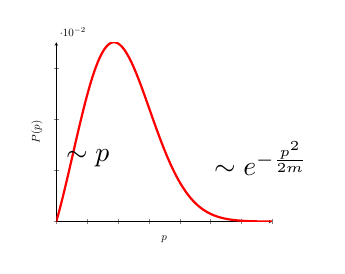
\begin{tikzpicture}[scale=0.4]
        
\begin{axis}[
    axis lines = left,
    xlabel = \(p\),
    ylabel = {\(P(p)\)},
     xticklabels={},
    yticklabels={},
]

\addplot [
    domain=0:35, 
    samples=100, 
    color=red,
    line width=2pt
]
{x*0.01*(exp{-(0.1*(x-4))^2})};

\end{axis}
\node[]at (1,2){$\sim p$};
\node[]at (6.5,2){$\sim e^{-\frac{p^2}{2m}}$};
\end{tikzpicture}
\end{center}
        

\item Nun gibt es Energieaustausch mit der Wand: Nach Stoß mit der Wand wird die Geschwindigkeit der Teilchen auf einen festen Betrag gesetzt, damit die Temperatur des Systems konstant bleibt. Nach einer gewissen Zeit stellt sich ein gleichgewicht Analog zu der eben gezeigten theoretischen Kurve ein. Allerdings gibt es einen weiteren Peak rechts des maximums: \\
Grund dafür ist, dass langsame Teilchen seltener zur Wand gelangen. Damit ist die durchschnittliche Geschwindigkeit, mit der Teilchen auf die Wand treffen, größer als die Durchschnittsgeschwindigkeit aller Teilchen.
\item Nun wird die Wand geheitzt. Nach einer gewissen Zeit stellt sich wieder ein Gleichgewicht ein.
        

\end{enumerate}
\end{beispiel}
\subsubsection{Energieverteilung im kanonischen Ensemble}
System habe eine Energie in $[E, E+ dE ]$. Wie groß ist WS $P(E) \ dE$?
\begin{align}
    P(E) \ dE &\propto \left[ M(E+dE) - M(E) \right] e^{- \beta E} \\
    \rightarrow \ P(E) &\propto \frac{dM(E)}{dE} e^{-\beta E} = \underbrace{d(E)}_{\text{Zustandsdichte}} \overbrace{e^{-\beta E}}^{\text{fällt für große E ab}}\\
    &\text{ideales Gas:  } d(E) \propto E^{\frac{3N}{2}-1} \\
    \Rightarrow &P(E) \text{ hat Minimum}
\end{align}

\begin{center}
\begin{tikzpicture}
\begin{axis}[
    axis lines = left,
    xlabel = \(E\),
    ylabel = {\(P(E)\)},
    xticklabels={},
    yticklabels={},every axis x label/.style={
    at={(ticklabel* cs:1.05)},
    anchor=west,},
every axis y label/.style={
    at={(ticklabel* cs:1.05)},
    anchor=south,}
]

\addplot [
    domain=0:7, 
    samples=100, 
    color=red,
]
{exp{-(2*(x-3))^2}};
\end{axis}

\draw[<->] (2.47,2.4)--(3.35,2.4) node[anchor=west] {$\Delta E \propto \sqrt{N}$};
\draw[-] (3,0.15)--(3,-0.15) node[anchor=north]{$\langle E \rangle \propto N$};
\end{tikzpicture}   
\end{center}
\begin{align*}
    &\text{relative Breite: } \frac{\Delta E}{\langle E \rangle} \propto \frac{\sqrt{N}}{N} = \frac{1}{\sqrt{N}} \\
    &\Rightarrow \text{kanonisches Ensemble} \stackrel{N \to \infty}{\longrightarrow} \text{ mikrokanonisches Ensemble}
\end{align*}

\vspace{1cm}
\color{black!50!white}
\textbf{Alternative Herleitung:}


\begin{wrapfigure}{r}{0.25\textwidth}
    \begin{center}
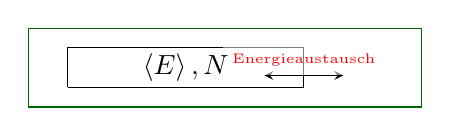
\begin{tikzpicture}[scale=0.5]
    \draw[green!40!black] (0,0)--(10,0)--(10,2)--(0,2)--(0,0);
    \draw (1,0.5)--(7,0.5)--(7,1.5)--(1,1.5)--(1,0.5);
    \draw[stealth-stealth] (6,0.8)--(8,0.8) node[above,midway, red, fill=white,opacity=.5,text opacity=1] {\tiny{Energieaustausch}};
    \draw (4,1) node {$\langle E\rangle \, ,N$};
\end{tikzpicture}
\end{center}
\end{wrapfigure}

Das kanonische Ensemble wurde hier mit dem postulierten Prinzip der maximalen Entropie eingeführt.
Die Herleitung kann auch ?rigoroser? erfolgen:\\
Das Gesamtsystem (inkl. Umgebung) kann mittels des mikrokanonischen Ensembles beschrieben werden, das es ein isoliertes System ist.
\\ Will man nun die WS eines Zustands im kleineren Teilsystems wissen, muss man sich folgendes überlegen:\\
Geht im Teilsystem ein Zustand in einen anderen Zustand über, ändert sich die Energie. Es kommt zum Austauschh mit der Umgebung.
\begin{itemize}
    \item Wird die Energie im Teilsystem größer, so muss sie in der Umgebung kleiner werden. Also hat die Umgebung eine hohe Zustandsdichte.
    \item Wird die Energie im Teilsystem kleiner, so wird die Energie in der Umgebung größer. Die Umgebung hat dann eine geringe Zustandsdichte.
\end{itemize}
Indem man die Anzahl an möglichen Zuständen in der Umgebung betrachtet, damit der eben beschreibene \enquote{ Energiefluss} passieren kann, können die selben Beziehungen für das kanonische Ensemble hergeleitet werden.
Damit wird das Prinzip der maximalen Entropie bestätigt.
\color{black}


\subsection{Großkanonisches Ensemble}\label{sec.Großkanonisches Ensemble}

\begin{center}
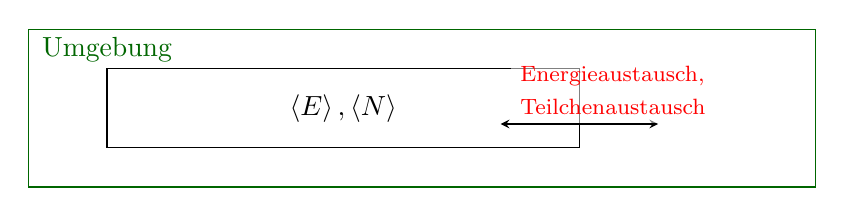
\begin{tikzpicture}
    \draw[green!40!black] (0,0)--(10,0)--(10,2)--(0,2)--(0,0);
    \draw (1,0.5)--(7,0.5)--(7,1.5)--(1,1.5)--(1,0.5);
    \draw[stealth-stealth] (6,0.8)--(8,0.8) node[above, red, fill=white,opacity=.5,text opacity=1, text width=3.5cm] {\footnotesize{Energieaustausch, \\Teilchenaustausch}};
    \draw (4,1) node {$\langle E\rangle \, , \langle N\rangle$};
    \draw (1,1.75) node[green!40!black] {Umgebung};
\end{tikzpicture}
\end{center}

Beispiele:
\begin{itemize}
    \item durchlässige Membran
    \item Elektronentransport
    \item Photonen im Hohlraum
    \item Adsorption
\end{itemize}


\textbf{Ziel:} Dichteoperator $\hat{\varrho}$ bzw. WS $p_n$ für Eigenzustand des Hamiltonoperators mit Energie $E_n$ und Teilchenzahl $N_n$.
\vspace{0.5cm}


Spezialfall: 
\begin{alignat}{2}
    A_1 &= \hat{H} \qquad \lambda_1 &&\rightarrow \beta \\
    A_2 &= \hat{N} \qquad \lambda_2 &&\rightarrow \alpha = - \beta \mu
\end{alignat}
mit $\hat{N}$ - Teilchenzahloperator und $\mu$ chemisches Potential (Eigenschaft der Umgebung)

\begin{equation}
    \fcolorbox{red}{white}{$\varrho_G = \frac{1}{Z} e^{-\beta H - \alpha N}$}
\end{equation}
\begin{equation}
    \fcolorbox{red}{white}{$Z_G(\beta,\alpha) = \trace(e^{-\beta H - \alpha N})$} = \trace(e^{- \beta (H-\mu N)})
\end{equation}
In der Basis der Eigenzustände $\{\ket{\phi_n}\}$:
\begin{equation}
    \fcolorbox{black}{white}{$p_n = \frac{1}{Z_G} e^{-\beta E_n - \alpha N_n}$} \qquad \fcolorbox{black}{white}{$Z_G(\beta, \alpha) = \sum_n e^{- \beta E_n - \alpha N_n}$} 
\end{equation}
Erwartungswerte:
\begin{equation}
    \langle N \rangle = - \frac{\partial}{\partial \alpha} \ln(Z_G(\beta,\alpha)) \quad , \quad \langle E \rangle = - \frac{\partial}{\partial \beta} \ln(Z_G(\beta,\alpha))
\end{equation}
Entropie:
\begin{align}
    S(\langle E \rangle,\langle N \rangle) &= k \ln(Z_G(\beta,\alpha)) + k \beta \langle E \rangle + k \alpha \langle N \rangle \\
    \frac{\partial S}{\partial \langle N \rangle} &= k \alpha = - k \beta \mu \color{black!50!white} = - \frac{\mu}{T} \color{black} \\
    \frac{\partial S}{\partial \langle E \rangle} &= k \beta \color{black!50!white} = \frac{1}{T} \color{black}
\end{align}



\begin{center}
    \begin{tikzpicture}
        \draw[->, line width=1.5pt] (-0.01,0) -- (5.2,0) node[right] {};
  \draw[->, line width=1.5pt] (0,-0.5) -- (0,3.5) node[above] {$E$};
  \draw[] (0,1)--(2.5,1){};
  \draw[] (0,1.5)--(2.5,1.5){};
  \draw[] (0,2)--(2.5,2){};
  \draw[] (0,3)--(2.5,3){};
  \draw[pattern=north west lines, pattern color=blue!50!white] (3,1.5) rectangle (6,2.2) ;
  \node[text width =3cm] at (6,1.75){$\mu$};
  \node[text width =3.5cm, right, blue] at (6,1.7) {\footnotesize{chemisches Potential\\ der Umgebung}};
  \draw[->] (3.2,2.2)  to [out=90,in=90] node[midway,above left,inner sep=2pt, red] {\tiny{Energiezufuhr}} (1,1);
  \draw[<-] (3.5,2.2)  to [out=90,in=90] node[midway,above right,inner sep=2pt, red] {\tiny{Energieabgabe}} (1,3);
    \end{tikzpicture}
\end{center}

\subsection{Fundamentale Fragen} \marginpar{VL. 10}
 \subsubsection{Gibbsches Paradoxon}

 
\begin{center}
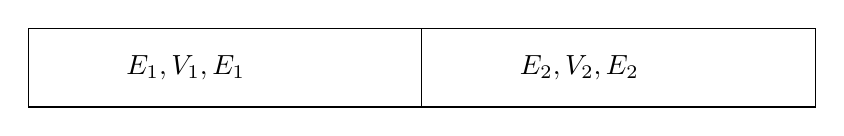
\begin{tikzpicture}
    \draw[black] (0,0)--(5,0)--(5,1)--(0,1)--(0,0);
    \draw (5,0)--(10,0)--(10,1)--(0,1);
    \draw (2,0.5) node {$E_1, V_1, E_1$};
    \draw (7,0.5) node {$E_2, V_2, E_2$};
\end{tikzpicture}
\end{center}

Zwei ideale Gase, gleiche Dichte $\frac{N_1}{V_1} = \frac{N_2}{V_2}$, im Mittel gleiche Energie pro Teilchen $\frac{E_1}{N_1} =\frac{E_2}{N_2}$, gleiche Massen $m_1=m_2$

\textbf{Frage:} Entropieänderung bei Herausnehmen der Wand?

\textbf{ideales Gas} (mikrokanonisch, klassisch, Kap. \ref{seq.Mikrokanonisches_ensemble}) ununterscheidbare Teilchen, d.h. ohne Faktor $\frac{1}{N!}$.
\begin{equation}
    M(E)= \frac{\int_{H(\Vec{q}, \Vec{p}) \leq E} d\Vec{p} d\Vec{q}}{h^{3N}} = \stackrel{\ref{seq.ideales Gas}}{...} = \stackrel{\text{Übung 7.2}}{...} = \left(\frac{V}{\lambda^3} e^{3/2}\right)^N
\end{equation}
mit \begin{equation}
    \lambda = \frac{h}{\sqrt{\frac{4}{3}} \pi m \frac{E}{N}}
\end{equation}

\color{black!50!white}
\paragraph{Bemerkung} für kanonisches Enseble mit $E= 3N \frac{1}{2} k T$ folgt:
\begin{equation}
    \fcolorbox{red}{white}{$\lambda = \frac{h}{\sqrt{2 \pi mkT}} \hspace{2cm} \text{thermische De-Broglie Wellenlänge}$}
\end{equation}

Nenner $\propto $ Impuls bei $kT$.
\color{black}

Entropie:
\begin{equation}\label{eq:Entropie_Gibsses Paradoxon}
    S(N,V,E) = k \ln{(M_{\Delta}(E))} \approx k \ln{(M(E))} = kN \left( \ln \left( \frac{V}{\lambda^3}\right) + \frac{3}{2}\right)
\end{equation}


\textbf{Erwartungen:}
\begin{itemize}
    \item[] $S_{\footnotesize{\textit{ohne Wand}}}^{\footnotesize{\textit{verschiedene Teilchen}}} > S_{\footnotesize{\textit{Wand}}}$  (, da ohne Wand größerer Mangel an Information)
    \item[] 
    \item[] $S_{\footnotesize{\textit{ohne Wand}}}^{\footnotesize{\textit{identische Teilchen}}} = S_{\footnotesize{\textit{Wand}}}$ (, da eigentlich keine Information gewonnen oder verloren wird)
\end{itemize}


\textbf{mit Wand:}
\begin{align}
    S_{\footnotesize{\textit{Wand}}} &= S(N_1,V_1,E_1) + S(N_2,V_2,E_2) \\&\stackrel{(\ref{eq:Entropie_Gibsses Paradoxon})}{=} k N_1 \ln\left(\frac{V_1}{\lambda^3}\right) + k N_2 \ln\left(\frac{V_2}{\lambda^3}\right) +k (N_1+N_2)^\frac{3}{2}
\end{align}

\textbf{ohne Wand, verschiedene Teilchen:}
\begin{align}
    S_{\footnotesize{\textit{ohne Wand}}}^{\footnotesize{\textit{verschiedene Teilchen}}} &= S(N_1,V_1+V_2,E_1) + S(N_2,V_1+V_2,E_2) \\&\stackrel{(\ref{eq:Entropie_Gibsses Paradoxon})}{=} k N_1 \ln\left(\frac{V_1+V_2}{\lambda^3}\right) + k N_2 \ln\left(\frac{V_1+V_2}{\lambda^3}\right) +k (N_1+N_2)^\frac{3}{2}\\
    &> S_{\footnotesize{\textit{Wand}}} \hspace{1cm} \Rightarrow \ \text{1. Erwartung bestätigt}
\end{align}

\textbf{ohne Wand, identische Teilchen:}
\begin{align}
    S_{\footnotesize{\textit{ohne Wand}}}^{\footnotesize{\textit{identische Teilchen}}} &= S(N_1+N_2,V_1+V_2,E_1+E_2)  \\&\stackrel{(\ref{eq:Entropie_Gibsses Paradoxon})}{=} k (N_1 +N_2)\ln\left(\frac{V_1+V_2}{\lambda^3}\right) +k (N_1+N_2)^\frac{3}{2} \\
    &= S_{\footnotesize{\textit{ohne Wand}}}^{\footnotesize{\textit{verschiedene Teilchen}}}\\
    &> S_{\footnotesize{\textit{Wand}}} \hspace{1cm} \Rightarrow \ \text{\Lightning Widerspruch zur 2. Erwartung}
\end{align}


\textbf{Lösung:}
Klassisch müssen wir in QM, identische Teilchen als ununterscheidbar angesehen werden.\footnote{Vorher: Naiv wurde angenommen, dass klassisch Teilchen unterschiedbar sein müssen. D.h., dass man im Phasenraum die Trajektorien aller Teilchen uneingeschränkt nachverfolgen kann. \\
Jetzt: Tatsächlich sind auch klassisch identische Teilchen nicht unterscheidbar.\\
In der QM werden Teilchen als Wellenpacket angenommen. Wenn diese sich vermischen bzw. ineinander laufen, sind diese danach ebenfalls nicht zu unterscheiden.}
\begin{itemize}
    \item[$\Rightarrow$] Permutation identischer Teilchen liefter keinen neuen Zustand
    \item[$\Rightarrow$] Faktor $\frac{1}{N!}$ bei Zahl der Zustände
    \item[$\Rightarrow$] \textbf{korrekte Formel für ideales Gas}
\end{itemize}
\begin{align}
    M(E) &= \frac{1}{N!} \ \frac{\int_{H(\Vec{q}, \Vec{p})<E} d\Vec{p}\, d\Vec{q}}{h^{3N}} \stackrel{\text{Stirling}}{\approx} \left( \frac{V}{N \lambda^3} e^{\frac{5}{2}} \right) ^N\\
    S&= k N \left( \ln\left(\frac{V}{N \lambda^3}\right) + \frac{5}{2}\right)
\end{align}

Löst Gibbsches Paradoxon (siehe Ü 7.2)






\subsubsection{Poincaré-Rückkehr Theorem}

\begin{definition}{Poincaré-Rückkehr Theorem}
    \textbf{Vorraussetzungen:}\\
    Hamiltonsystem mit \underline{endlichen} Phasenraumvolumen bei $H(\Vec{q}, \Vec{p}) = E$.

    \begin{tcolorbox}[colback=red!10!white,colframe=red!10!white]
    Phasenraumpunkte, die ein Phasenraumgebiet $\Gamma_0$ verlassen, kommen irgendwann (fast alle) wieder zurück nach $\Gamma_0$. \\
    Außnahmen, die nicht zurück kommen, haben Volumen Null.
    \end{tcolorbox}
\end{definition}

\begin{center}
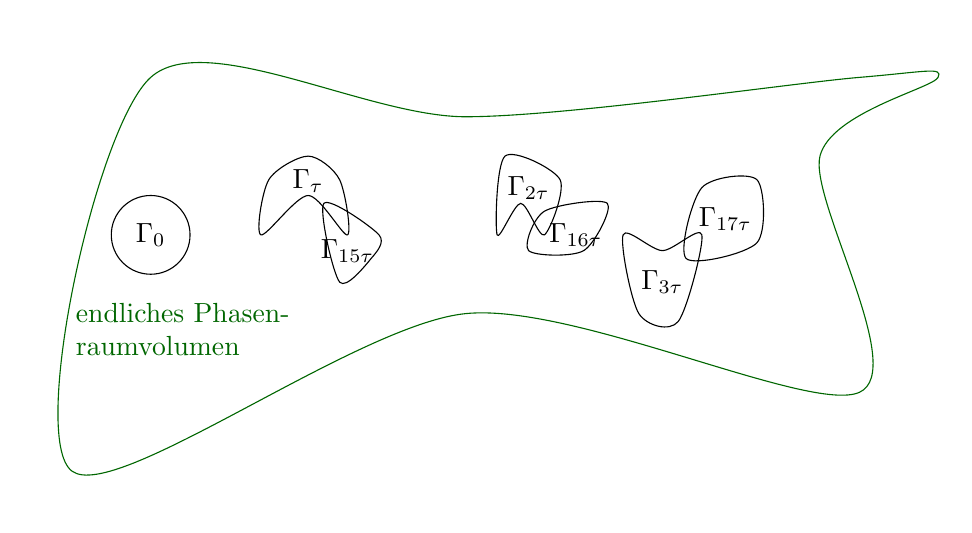
\begin{tikzpicture}
 \draw [green!40!black] plot [smooth cycle] coordinates {(0,0) (5,2) (10,1) (9.5,4) (11,5) (10,5) (5,4.5)  (1,5)};
    \draw (1.8,1.8) node[green!40!black, text width=3.5cm] {endliches Phasenraumvolumen};
    \draw (1,3) circle[radius = 0.5] node {$\Gamma_0$}; 
    \draw plot [smooth cycle] coordinates {(2.4,3) (3,3.5) (3.5,3) (3.4,3.7) (3,4) (2.5,3.7)} node at (3,3.68) {$\Gamma_{\tau}$};
    \draw plot [smooth cycle] coordinates {(3.4,2.4) (3.8,2.7)  (3.9,3) (3.2,3.4)} node at (3.5,2.8) {$\Gamma_{15\tau}$};
    \draw plot [smooth cycle] coordinates {(5.4,3) (5.7,3.4) (6,3) (6.2,3.7)  (5.5,4)} node at (5.8,3.6) {$\Gamma_{2\tau}$};
      \draw plot [smooth cycle] coordinates {(6,3.3) (6.8,3.4) (6.5,2.8) (5.8,2.8)  } node at (6.4,3) {$\Gamma_{16\tau}$};
    \draw plot [smooth cycle] coordinates {(7.2,2) (7.7,1.9) (8,3) (7.5,2.8) (7,3)} node at (7.5,2.4) {$\Gamma_{3\tau}$};
    \draw plot [smooth cycle] coordinates {(7.8,2.7) (8.7,2.9) (8.7,3.7) (8,3.6) } node at (8.3,3.2) {$\Gamma_{17\tau}$};
\end{tikzpicture}
\end{center}

\begin{proof}{Lemma: \textit{ mindestens ein Teilvolumen kehrt zurück.}}\label{Lemma_poincare}\\
    Annahme: Zur Zeit $\tau$ gelte für zeitentwickeltes Gebiet $\Gamma_{\tau}: \hspace{1cm}\Gamma_{\tau} \cap \Gamma_0 = \emptyset $.\\
    Nach \textbf{Lioville Therorem} sind die Volumina $\Gamma_0, \Gamma_{\tau}, \Gamma_{2\tau}, ...$ gleich groß. Das erreichbare Phasenraumvolumen ist allerdings endlich.
\begin{align*}
    \Rightarrow & \exists m,n : & &\Gamma_{m \tau} \cap \Gamma_{n\tau} &\text{ hat Volumen > 0} \\
     \Rightarrow &  & &\Gamma_{(m-1 )\tau} \cap \Gamma_{(n-1)\tau} &\text{ hat Volumen > 0} \\
     \Rightarrow& ... &&&\\
      \Rightarrow &  & &\Gamma_{(m-n) \tau} \cap \Gamma:{0} &\text{ hat Volumen > 0} \\
\end{align*}
$\Rightarrow$ Ein Teil von $\Gamma_0$ mit Volumen >0 ist nach Zeit $(m-n) \tau$ zurückgekommen
\end{proof}
\begin{proof}{Poincaré-Rückkehr Theorem durch Widerspruch}
    Angenommen, es gäbe ein Volumen >0, das nicht zu $\Gamma_0$ zurückkommt $\stackrel{\textit{Lemma}}{\Rightarrow}$ Teilvolumen davon kommt zu $\Gamma_0$ zurück. \Lightning
\end{proof}

\textbf{Bemerkung:}
\begin{itemize}
    \item Macht keine Aussage für einzelne Phasenraumpunkte (einzelner Phasenraumpunkt kommt ggf. nie zurück) \footnote{Beachte: In einem $N$-dimensionalen Phasenraum bildet eine $N-1$-dimensionale Hyperfläche nach dem hier verwendeten Lebesquemaß eine Nullmenge.}
    \item Verteilung der Rückkehrzeit ?
    \item hat für hohe Dimensionen (z.B. $10^2^3$) keine praktische Relevanz
\end{itemize}

\begin{beispiel}{Pendel}
        \begin{center}
        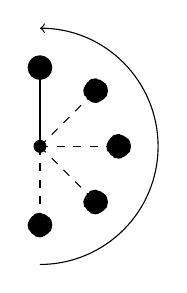
\begin{tikzpicture}
            \draw (0,0) node [circle, draw = black, fill = black,inner sep=1.5pt] {};
            \draw[dashed] (0,0) --(0,-1) node (0,-1) [circle, draw = black, fill = black,inner sep=3pt] {};
            \draw[dashed] (0,0) --(0.707,-0.707) node ((0.707,-0.707) [circle, draw = black, fill = black,inner sep=3pt] {};
            \draw[dashed] (0,0) --(1,0) node (1,0) [circle, draw = black, fill = black,inner sep=3pt] {};
            \draw[dashed] (0,0) --(0.707,0.707) node ((0.707,0.707) [circle, draw = black, fill = black,inner sep=3pt] {};
            \draw (0,0) --(0,1) node (0,1) [circle, draw = black, fill = black,inner sep=3pt] {};
            \draw [->](0,-1.5) arc (-90:90:1.5);
        \end{tikzpicture}
    \end{center}

Ein Pendel kann so ausgelenkt werden, dass es im instabilen Gleichgewicht genau oben stehen bleibt. Dieser Phasenraumpunkt wird also nie zurückkehren. Es gibt unendlich viele Phasenraumpunkte dieses Pendels (von einem bestimmten Ort mit der passenden Geschwindigkeit) so auszulenken, sodass es oben stehen bleibt.

Diese Punkte bilden im gesamten Phasenraum allerdings eine Nullmenge.
\end{beispiel}



\subsubsection{Ergodenhypothese} \marginpar{VL 11}
\begin{itemize}
    \item[Problem] klassische Erwartungswerte ergeben sich aus Ensemblemittel (Phasenraummittel)
    \item[Idee]/Hoffnung: Trajektorie durchläuft zeitlich den gesamten Phasenraum gleichmäßig, d.h.
    \begin{align}
        &\text{Phasenraummittel} &= \quad &\text{Zeitmittel} \\
        &\frac{\int \, \varrho(\Vec{q},\Vec{p}) f(\Vec{q},\Vec{p}) \, d\Vec{q}d\Vec{p}}{\int \, \varrho(\Vec{q},\Vec{p}) \, d\Vec{q}d\Vec{p}} & &\lim_{\tau \to \infty} \frac{1}{\tau} \int_0^{\tau} \, f(\Vec{q}(t),\Vec{p}(t)) \, dt
    \end{align}
\end{itemize}
\begin{definition}{Ergodizität}
    $\exists$ WS-Dichte $\varrho(\Vec{q},\Vec{p})$, so dass Phasenraummittel = Zeitmittel für beliebig Observale und für fast alle Trajektorien
    \begin{equation}
        \langle f(\Vec{q},\Vec{p}) \rangle_{\Gamma} = \langle f(\Vec{q}(t),\Vec{p}(t)) \rangle_t
    \end{equation}
\end{definition}

\begin{prop}{Ergodenhypothese}
    Annahme der Ergodizität in makroskopischen Systemen
\end{prop}
Sind hamiltonische Systeme wirklich ergodisch?

\begin{beispiel}{ergodische Systeme}
    \begin{itemize}
    \item System mit 1 Freiheitsgrad:
\begin{center}
    \begin{tikzpicture}
  \draw[->, thick] (-0.01,0) -- (4.2,0) node[right] {$x$};
  \draw[->, thick] (0,-0.5) -- (0,1.5) node[above] {$E$};
  \draw[color=red, <->]   (1.14,0.5)--(3.14,0.5)   node[right] {$E_1$};
  \draw[dashed] (3.14,0) --(3.14,1);
  \draw[dashed] (1.14,0) --(1.14,1);
  \node[below] at (3.14,0) {$L$};
\end{tikzpicture}
\end{center}
    offensichtlich ist Zeitmittel=Phasenraummittel, da $\Vec{p}$ nur von rechts nach links oder umgekehrt zeigen kann und $\abs{\Vec{v}} = const.$.\\
    Damit wird der gesamte Phasenraum durch abgedeckt.
    \item System mit 2 Freiheitsgraden

    \begin{center}
        \begin{tikzpicture}
            \draw (0,2)--(0,0)--(4,0)--(4,2);
            \draw plot [smooth] coordinates{(0,2) (1,2) (2,2.5) (3,2) (4,2)};
        \end{tikzpicture}
    \end{center}
    Es gibt Bereiche (im Phasenraum) mit regulärer Dynamik und Bereiche chaotischer Dynamik $\rightarrow$ nicht ergodisch
    \item man kann immer eine Observable f finden, so dass System \enquote{ergodisch} ist, aber für tatsächliche Ergodizität muss diese Eigenschaft für \textbf{alle} Observablen gelten
    \item i.A. wird angenommen, dass Systeme mit sehr vielen ($~10^{23}$) Freiheitsgraden ergodisch sind, allerdings sind auch Ausnahmen bekannt und das ist nicht bestätigt
    \item Ergodizität kann auch für QM formuliert werden
\end{itemize}
\end{beispiel}

\subsubsection{Irreversibilität}
In der Natur ist eine bestimmte Zeitrichtung natürlicherweise ausgezeichnet: Wir altern usw... Allerdings zeichnet sich ein Hamilton’sches System durch die Invarianz unter Zeitumkehr aus.
\begin{itemize}
    \item Beispiel TUD Logo:
    \begin{itemize}
        \item am Anfang TUD Logo im Billard aus Kugeln
        \begin{center}
            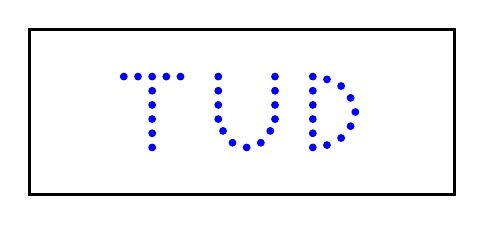
\begin{tikzpicture}[scale=0.60]
                \draw[very thick] (-1,0) rectangle (8,3.5);
                \filldraw[blue] (1,2.5) circle (2pt);
                \filldraw[blue] (1.3,2.5) circle (2pt);
                \filldraw[blue] (1.6,2.5) circle (2pt);
                \filldraw[blue] (1.9,2.5) circle (2pt);
                \filldraw[blue] (2.2,2.5) circle (2pt);
                \filldraw[blue] (1.6,2.2) circle (2pt);
                \filldraw[blue] (1.6,1.9) circle (2pt);
                \filldraw[blue] (1.6,1.6) circle (2pt);
                \filldraw[blue] (1.6,1.3) circle (2pt);
                \filldraw[blue] (1.6,1.0) circle (2pt);
                \filldraw[blue] (3,2.5) circle (2pt);
                \filldraw[blue] (3,2.2) circle (2pt);
                \filldraw[blue] (3,1.9) circle (2pt);
                \filldraw[blue] (3,1.6) circle (2pt);
                \filldraw[blue] (3.1,1.35) circle (2pt);
                \filldraw[blue] (3.3,1.1) circle (2pt);
                \filldraw[blue] (3.6,1) circle (2pt);
                \filldraw[blue] (4.2,2.5) circle (2pt);
                \filldraw[blue] (4.2,2.2) circle (2pt);
                \filldraw[blue] (4.2,1.9) circle (2pt);
                \filldraw[blue] (4.2,1.6) circle (2pt);
                \filldraw[blue] (4.1,1.35) circle (2pt);
                \filldraw[blue] (3.9,1.1) circle (2pt);
                \filldraw[blue] (5,2.2) circle (2pt);
                \filldraw[blue] (5,2.5) circle (2pt);
                \filldraw[blue] (5,1.9) circle (2pt);
                \filldraw[blue] (5,1.6) circle (2pt);
                \filldraw[blue] (5,1.3) circle (2pt);
                \filldraw[blue] (5,1.0) circle (2pt);
                \filldraw[blue] (5.3,2.44) circle (2pt);
                \filldraw[blue] (5.6,2.3) circle (2pt);
                \filldraw[blue] (5.8,2.05) circle (2pt);
                \filldraw[blue] (5.9,1.75) circle (2pt);
                \filldraw[blue] (5.8,1.45) circle (2pt);
                \filldraw[blue] (5.6,1.2) circle (2pt);
                \filldraw[blue] (5.3,1.05) circle (2pt);
            \end{tikzpicture}
        \end{center}
        \item Start der Kugeln mit zufälligen Anfangsbedingungen
        \item nach gewisser Zeit Zeitumkehr
        \item[$\Rightarrow$] je nach Zeitpunkt TUD Logo gut bis gar nicht zu erkennen
        \item[$\rightarow$] chaotisches System, Abweichungen durch Potenzierung der Ungenauigkeiten durch endliche Genauigkeit bei der Rechnung 
    \end{itemize}
\end{itemize}

\subsubsection{Maxwell Dämon}
\begin{itemize}
    \item System mit getrennten Kammern, Trennung: Tür die nur von einer Seite durchlässig ist (Dämon öffnet und schließt die Tür je nachdem von wo das Teilchen kommt)
    \item nach gewisser Zeit ist Druck auf der einen Seite höher
    \item[$\Rightarrow$] Druckausgleich zur Energiegewinnung
    \item[$\Rightarrow$] Perpetuum mobile 
\begin{table}[h]
    \centering
    \begin{tabular}{c|c}
        Variante 1 & Variante 2 \\ \hline
        Gas homogen verteilt & Gas homogen verteilt \\
        A $\rightarrow$ B $\Rightarrow$ Tür offen & A $\rightarrow$ B, wenn $v > v_0$ \\
        B $\rightarrow$ A $\Rightarrow$ Tür zu & B $\rightarrow$ A, wenn $v \leq v_0$ \\
        $\stackrel{\text{Zeit}}{\Rightarrow}$ mehr Teilchen in B & $\stackrel{\text{Zeit}}{\Rightarrow}$ langsame Teilchen in A, T klein \\
        $\Rightarrow$ Energiegewinnung durch Druckausgleich & $\Rightarrow$ schnelle Teilchen in B, T groß
    \end{tabular}
    \label{tab:Maxwell Dämon}
\end{table}
    \item[$\Rightarrow$] Heizung / Energiegewinnung
\end{itemize}

$\rightarrow$ Problem: Tür auf molekularer Ebene bauen

\subsubsection{Feynman-Ratsche}
\begin{itemize}
    \item[] Nutzung einer Ratsche (nur Bewegung in eine Richtung möglich). Damit stellt sich die Frage: Kann man aus der thermischen Bewegung eine gerichtete Bewegung erzeugen?
    \item[]
    \item[] Problem: auch das Ratschen-Blatt fluktuiert thermisch, sodass Ratsche auch zurück kann
    \item[]
    \item[] \textbf{Im Allgemeinen:} Das sind Gedankenexperimente, die (noch) nicht realisert werden konnten und die auch sehr schwer zu realisieren scheinen, allerdings ist nicht bewiesen wurden, dass sie nicht funktionieren.
\end{itemize}






\section{Thermodynamik} \marginpar{VL 12}

\begin{center}
    \emph{Wie passt die statistische Physik zur Thermodynamik?}
\end{center}

\begin{itemize}
    \item makroskopisch scheint alles deterministisch und ohne statistischen Ursprung
    \item Übertragung der thermodynamischen Konzepte auf mikroskopische Größen
    \begin{itemize}
        \item[]kein Problem: Impuls, Schwerpunkt, Teilchenzahl, innere Energie $U = \langle H \rangle$
        \item[]schwieriger: Temperatur, Druck, Wärme, thermodynamische Entropie 
    \end{itemize}
    \item Hauptsätze der Thermodynamik statistisch begründen
\end{itemize}

\subsection{0. Hauptsatz}
\begin{definition}{0. Hauptsatz}
    Zwei Systeme, die jeweils im thermischen Gleichgewicht mit einem dritten System sind, befinden sich auch untereinander im Gleichgewicht.
\end{definition}
Beschreibung in der statistischen Physik (kanonisches Ensemble):
\begin{itemize}
    \item zwei Systeme im Gleichgewicht zur Umgebung (3. System)
    \begin{itemize}
        \item[] System a:
        \begin{align}
            \varrho_a &= \frac{1}{Z_a(\beta_a)} e^{-\beta_a H_a} \\
            \underbrace{U_a}_{\langle E \rangle} &= - \pd{}{\beta_a} \ln\left( Z_a(\beta_a) \right) \: \Rightarrow \: \beta_a(U_a)
        \end{align}
        \item[] System b:
        \begin{align}
            \varrho_b &= \frac{1}{Z_b(\beta_b)} e^{- \beta_b H_b} \\
            U_a &= - \pd{}{\beta_b} \ln\left( Z_b(\beta_b) \right) \: \Rightarrow \: \beta_b(U_b)
        \end{align}
        \item[$\rightarrow$] $\beta_a \stackrel{?}{=} \beta_b$ 
    \end{itemize}
    \item Gesamtsystem $a+b$ in thermischen Kontakt:
    \begin{equation}
        H = H_a \otimes \mathds{1} + \mathds{1} \otimes H_b + V_{ab}
    \end{equation}
    \begin{itemize}
        \item[] $V_{ab}$ ist WW-Term, erlaubt Energieaustausch, $V_{ab} \ll H_a, H_b$ (beliebig klein)
    \end{itemize}
    \item[] Gesamtsystem an Umgebung gekoppelt: Gleichgewicht kanonisch
    \begin{align}
        \varrho_{a+b} &= \frac{e^{-\beta H}}{Z} = \frac{e^{-\beta\left(H_a \otimes \mathds{1} + \mathds{1} \otimes H_b + V_{ab}\right)}}{Z(\beta)} \\
        &\approx \frac{e^{-\beta H}}{Z} = \frac{e^{-\beta\left(H_a \otimes \mathds{1} + \mathds{1} \otimes H_b\right)}}{Z_a(\beta_a)\cdot Z_b(\beta_b)} \\
        \color{black!50} \text{NR: } Z(\beta) &= \color{black!50} \trace\left(e^{-\beta(\dots)}\right) = \sum_{m,n} \langle n,m| e^{-\beta(H_a \otimes \mathds{1} + \mathds{1} \otimes H_b )} \underbrace{|n,m\rangle}_{\ket{n}\ket{m}}\\
        \color{black!50} &= \color{black!50} \sum_{n,m} e^{-\beta H_n^a} e^{-\beta H_m^b} = Z_a(\beta) \cdot Z_b(\beta) \\
        &= \varrho_a(\beta) \otimes \varrho_b(\beta) \\
        &\Longrightarrow \beta = \beta_a = \beta_b
    \end{align}
\end{itemize}

\subsection{1. Hauptsatz}
\begin{definition}{1. Hauptsatz}
    \begin{itemize}
        \item[] Energieerhaltung
        \begin{equation}
            \Delta U = \Delta Q + \Delta W
        \end{equation}
        \item[] differentiell
        \begin{equation}
            dU = \delta Q + \delta W
        \end{equation}
        \begin{itemize}
            \item[]$dU$: exaktes Differential (totales Differential), vom Weg unabhängig
            \begin{itemize}
                \item[] Kreisprozess: $\oint \ dU = 0$
                \item[]
                \item[] $U$ Zustandsgröße, $U = \trace\left(\varrho H \right)$
            \end{itemize}
            \item[]$\delta Q, \delta W$: inexakte Differentiale, vom Weg abhängig
            \begin{itemize}
                \item[] Kreisprozess: $\oint \ \delta Q = -\oint \delta W \stackrel{i.A.}{\neq} 0$
                \item[]
                \item[] $Q,W$ keine Zustandsgrößen
            \end{itemize}
        \end{itemize}
    \end{itemize}
\end{definition}

\begin{beispiel}{Beispiel}
    zwei verschiedene Prozesse mit gleicher Zustandsänderung $\Delta U$
    \begin{enumerate}
        \item Gas wird Wärme $\delta Q = \Delta U$ zugeführt
        \item oszillierender Kolben (schnell): $\delta W = \Delta U$
    \end{enumerate}
    $\Rightarrow$ Erhöhung der inneren Energie, aber $\delta Q$ und $\delta W$ unbekannt, da keine Zustandsgrößen
\end{beispiel}

\paragraph{Wichtige Zustandsänderungen}
\begin{itemize}
    \item \emph{quasistatisch}: so langsam, dass immer im Gleichgewicht
    \item \emph{adiabatisch}: bei thermischer Isolation
\end{itemize}

\subsubsection{Was ist Wärme?}
\begin{itemize}
    \item System sei sei durch festes $H$ beschrieben, d.h. es wird keine Arbeit zugeführt ($\delta W = 0$)
    \item Kopplung an Umgebung (Wärmeübertragung) ändert $\varrho$
    \begin{align}
        U &= \trace\left(\varrho H\right) \stackrel{G.G.}{=} \sum_n p_n E_n \\
        dU &= \underbrace{\trace(d\varrho \: H)}_{\delta Q} + \underbrace{\trace(\varrho \: dH)}_{\delta W \text{ (hier = 0)}} \\
        \rightarrow \delta Q = \trace(d\varrho \: H) = \sum_n dp_n E_n
    \end{align}
\end{itemize}

Wärmezufuhr entspricht Umverteilung der Wahrscheinlichkeiten $p_n$ für Mikrozustände (während Wärmeübertragung $\rightarrow$ kein Gleichgewicht)\\
$\longrightarrow$ meist nicht reversibel


\subsubsection{Was ist Arbeit?}
\begin{itemize}
    \item System tauscht keine Wärme aus ($\delta Q = 0$)
    \item makroskopische Variablen $\xi_i$ werden extrem geändert
    \begin{align}
        H &= H(\{\xi_i\}) \rightarrow dH = \sum_i \underbrace{\pd{H}{\xi_i}}_{\chi_i} d\xi_i \\
        dU &= \underbrace{\trace(d\varrho \: H)}_{\delta Q \text{ (hier = 0)}} + \underbrace{\trace(\varrho \: dH)}_{\delta W} \\
        \delta W &= \color{black!50} \underbrace{\color{black}\trace(\varrho \: dH) \color{black!50}} \color{black} = \sum_n p_n \ dE_n \\
        & \color{black!50} \trace(\varrho \sum_i \chi_i \ d\xi_i) = \sum_i \trace(\varrho \chi_i) d\xi_i = \sum_i \langle \chi_i \rangle d\xi_i
    \end{align}
\end{itemize}

\begin{center}
    \begin{tikzpicture}[scale=0.9]
        \draw[thick] (0,0) -- (5,0) -- (5,2) -- (0,2);
        \filldraw[pattern=north east lines] (1,2) rectangle (0.75,0) node[anchor= north west]{$\xi$};
        \draw[<-,thick] (1.5,1) -- (0,1) node[anchor=east]{$\Vec{F}$};
    \end{tikzpicture}
\end{center}
\begin{equation}
    \delta W = F \ ds = - p \ dV = \mu \ dN
\end{equation}
\vspace{1cm}
\begin{itemize}
    \item[$\longrightarrow$] meist reversibel
    \item[$\longrightarrow$] Wärmezufuhr nicht reversibel 
\end{itemize}



\subsubsection{Exakte und inexakte Differentiale}
\paragraph{Exaktes (vollständiges, totales) Differential:}

Sei $F(x,y)$ Funktionen von 2 Veränderlichen
\begin{wrapfigure}{l}{2cm}
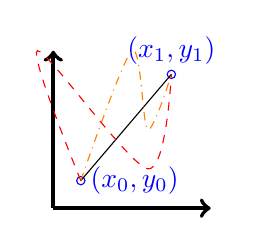
\begin{tikzpicture}
\coordinate (a) at (0.35,0.35);
\node[right, color=blue] at (a) {$(x_0,y_0)$};
\coordinate (b) at (1.5,1.7);
\node[above, color=blue] at (b) {$(x_1,y_1)$};
\draw[blue] (a) circle (1.5pt);
\draw[blue] (b) circle (1.5pt);
\draw[->, line width =1.5pt] (0,0)--(2,0);
\draw[->, line width =1.5pt] (0,0)--(0,2);
\draw (a)--(b);
      \draw[dash dot,orange] plot [smooth] coordinates {(a) (1,2)  (1.2,1) (b)};
       \draw[dashed, red] plot [smooth] coordinates {(a) (-0.2,2)  (1.2,0.5) (b)};
\end{tikzpicture}
 \end{wrapfigure}
\begin{align}
    dF &= \pd{F(x,y)}{x} \, dx + \pd{F(x,y)}{y} \, dy \\
    \int_{x_0,y_0}^{x_1,y_1} dF &= F(x_1,y_1) - F(x_0,y_0) = \text{wegunabhängig}
\end{align}
\begin{equation}
    \frac{\partial^2 F(x,y)}{\partial y \partial x} \stackrel{\text{Satz v. Schwarz}}{=} \frac{\partial^2 F(x,y)}{\partial x \partial y}
\end{equation}

\paragraph{Inexaktes (unvollständiges) Differential:}
\begin{align}
    \delta G &= a(x,y) \ dx + b(x,y) \ dy \\
     \int_{x_0,y_0}^{x_1,y_1} \delta G &= \text{wegabhängig}\\
     \text{da } &\nexists G(x,y) \text{ mit } \pd{G(x,y)}{x} = a(x,y) \quad \pd{G(x,y)}{y} = b(x,y) \\
     \Big( &\text{außer falls } \pd{a}{y} = \pd{b}{x} \Leftrightarrow \frac{\partial^2 G(x,y)}{\partial y \partial x} = \frac{\partial^2 G(x,y)}{\partial x \partial y} \Leftrightarrow \exists G \Big)
\end{align}

Integrierender Faktor $I(x,y)$:
\begin{align}
    I(x,y) \ \delta G &= I(x,y) \ a(x,y) \ dx + I(x,y) \ b(x,y) \ dy \\
    &\text{mit } \pd{}{y}\left( I(x,y) \ a(x,y) \right) \stackrel{!}{=} \pd{}{x}\left( I(x,y) \ b(x,y) \right) \\
    &\Rightarrow \text{ exaktes Differential } dF = I(x,y) \delta G
\end{align}

\begin{beispiel}{Beispiel aus der Thermodynamik}
    \begin{equation}
        dS = \underbrace{\frac{1}{T}}_{\text{integrierender Faktor}} \quad \delta Q
    \end{equation}
\end{beispiel}


\subsection{2. Hauptsatz}\marginpar{VL 13}
Motivation: Energieerhaltung (1. HS) erlaubt viele Prozesse, die aber nicht vorkommen, z.B. $\text{Wärme} \longrightarrow \text{Energie}$

\begin{definition}{2. Hauptsatz}
    Äquvalente Formulierungen:
    \begin{itemize}
        \item Kelvin 1854:
        \begin{quote}
            Ein Prozess, dessen einziges Endergebnis ist, einer Quelle Wärme zu entziehen und in Arbeit zu verwandeln ist unmöglich.
        \end{quote}
        \item Clausius 1854:
        \begin{quote}
            Ein Prozess, dessen einziges Endergebnis ein Wärmetransfer von kalt nach warm ist, ist unmöglich.
        \end{quote}
        \item Carnot 1824:
        \begin{quote}
            Wirkungsgrad $\eta$ einer Wärmekraftmaschine mit zwei Wärmebädern $T_1 > T_2$:
            \begin{equation}
                \eta \leq \frac{T_1-T_2}{T_1} = 1- \frac{T_2}{T_1} 
            \end{equation}$\Longrightarrow$ absolute Temperatur
        \end{quote}
        \item Clausius 1865:
        \begin{quote}
            Im thermodynamischen Gleichgewicht wird ein System durch Temperatur $T$ und Entropie $S$ beschrieben. In eienm quasistatischen Prozess gilt:
            \begin{equation}
                dS = \frac{\delta Q}{T}
            \end{equation}
            2. HS: Jeder andere nicht quasistatische Weg von Gleichgewicht 1 zu Gleichgewicht 2 ist irreversibel:
            \begin{equation}
                S_2 - S_1 \geq \sum_j \int \frac{\overbrace{\delta Q}^{\text{Wärmemenge von Bad j}}}{\underbrace{T}_{\text{Temperatur von Bad j}}}
            \end{equation}
            Wärmeisoliertes System: $\delta Q = 0$
            \begin{equation}
                \Rightarrow S_2 \geq S_1 \qquad (\text{Entropie kann nicht abnehmen})
            \end{equation}
        \end{quote}
    \end{itemize}
\end{definition}

\paragraph{Bemerkung zu Temperatur und thermodynamischer Entropie $S_{th}$}
\begin{itemize}
    \item beide nur bis auf Faktor definiert
    \item $S_{th}$ nur bis auf additive Konstante definiert (wird im 3. HS festgelegt)
\end{itemize}

\paragraph{Zusammenhang Temperatur $T$ aus Thermodynamik und $\beta$ aus statistischer Physik:}
quasistatische Prozesse $\Longrightarrow$ $\varrho$ im Gleichgewicht
\begin{align}
    \varrho &= \frac{e^{-\beta H}}{Z} \qquad S = - k \trace(\varrho \ln(\varrho)) \\
    &\text{\color{black!50} geht, da in GG $\Rightarrow$ in EZ ausdrücken} \\
    \Rightarrow dS &= - k \trace(d\varrho \: \underbrace{\ln(\varrho)}_{-\ln(Z) - \beta H}) - \underbrace{ k \trace(d\varrho)}_{=0} \\
    &\color{black!50} \trace(\varrho) = 1 \Rightarrow \trace(d\varrho) = 0\\
    dS &= k \ln(Z) \underbrace{\trace(d\varrho)}_{=0} + k \beta \underbrace{\trace(d\varrho \: H)}_{\delta Q = T dS_{th}} \\
    dS &= k T \beta dS_{th} \\
    &\Longrightarrow \beta = \frac{1}{kT} \cdot \underbrace{const.}_{\text{wähle 1}} \qquad \text{und } \ S = S_{th} + const.
\end{align}
$\Longrightarrow$ Äquivalenz von $\beta, \ S$ und $T, \ S_{th}$ bis auf Faktor und additive Konstante bei der Entropie

\paragraph{Bemerkung:}
\begin{itemize}
    \item 2. HS für isoliertes System ($\delta Q = 0$): $dS \geq 0$
    \begin{itemize}
        \item[$\widehat{=}$] Prinzip der maximalen Entropie der statistischen Physik
    \end{itemize}
    \item Entropie im kanonischen Ensemble (\ref{sec.Kanonisches Ensemble})
    \begin{align}
        S(\langle E\rangle) &= k \ln(Z) + \underbrace{k \beta}_{\frac{1}{T}} \underbrace{\langle E \rangle}_{E} \\
        \pd{S(E)}{E} &= \frac{1}{T}\\
        &\text{Definition der Temperatur in der statistischen Physik}
    \end{align}
    \item Entropie im Großkanonischen Ensemble (\ref{sec.Großkanonisches Ensemble})
    \begin{align}
        S(\langle E \rangle, \langle N \rangle) &= k \ln(Z_G) + \underbrace{k \beta}_{\frac{1}{T}} \langle E \rangle + \underbrace{k \alpha}_{-\frac{1}{T} \mu} \langle N \rangle \\
        \pd{S(E,N)}{E} &= \frac{1}{T} \\
        \pd{S(E,N)}{N} &= - \frac{1}{T} \mu
    \end{align}
\end{itemize}

\subsection{3. Hauptsatz}
\begin{definition}{3. Hauptsatz}
    Nernst 1906:
    \begin{quote}
        Bei $T=0$ ist Entropie unabhängig von Parametern $\xi_i$ von $H(\{\xi_i\})$
    \end{quote}
    äquivalente Aussage:
    \begin{quote}
        Der absolute Temperatur-Nullpunkt ist mit endlicher Zahl von Schritten nicht erreichbar.
    \end{quote}
    Planck:
    \begin{quote}
    Wähle additive Konstante der Entropie so, dass $S_{th}(T=0) = 0$
    \end{quote}
    \begin{align}
        \Rightarrow S_{th} &= S \\
        p_m &= \frac{e^{-\beta E_m}}{\sum_n e^{-\beta E_n}} = \frac{e^{-\beta (E_m-E_0)}}{\sum_n e^{-\beta (E_n-E_0)}} \quad E_0 - \text{Grundzustandsenergie}\\
        p_m &\stackrel{T \to 0, \beta \to \infty}{\longrightarrow} \begin{cases}
            0 \quad, m > 0 \\ 1 \quad, m = 0
        \end{cases} \Rightarrow S = - k \sum_m p_m \ln(p_m) = 0 \\
        &\text{unabhängig von $E_m$, d.h. von Systemparametern $\xi_i$} \quad \checkmark \\
        &\text{\color{black!50} (funktioniert auch bei Entartung)}
    \end{align}
\end{definition}

\begin{beispiel}{Beispiel ideales Gas klassisch}
    \begin{align}
        S &= kN \left( \ln\left(\frac{V}{N \lambda^3}\right) + \frac{5}{2}\right) \quad \text{mit } \lambda = \frac{h}{\sqrt{2 \pi m k T}} \\
        &\Rightarrow S \stackrel{T\to 0} - \infty \\
        &\color{black!50} \Rightarrow \varrho(\Vec{q},\Vec{p}) = \frac{e^{-\beta H(\Vec{q},\Vec{p})}}{Z}\\
        &\color{black!50} \rightarrow \text{Wahrscheinlichkeitsdichte zieht sich auf Punkt im Phasenraum zusammen}\\
        &\color{black!50} \rightarrow \text{passt nicht mehr mit Planck-Zelle zusammen}\\
        &\rightarrow \text{Widerspruch zum 3. HS}\\
        &\Longrightarrow \text{q.m. Rechnung für $T\to 0$ notwendig!}
    \end{align}
\end{beispiel}

\subsection{Thermodynamischer Limes}
\begin{definition}{Thermodynamischer Limes}
\begin{itemize}
    \item System groß gegenüber mikroskopischen Abständen
    \item viele Teilchen $N\to \infty$, aber $\frac{N}{V}=const.$
    \item Oberflächeneffekte vernachlässigbar
    \item Form unwichtig, Volumen ausreichende Beschreibung
\end{itemize}

\paragraph{Extensive Variablen}:
\begin{itemize}
    \item[] proportional zum Volumen
    \begin{itemize}
        \item[Bsp.:] Teilchenzahl, Volumen, Entropie, Innere Energie, Masse, Impuls
    \end{itemize}
\end{itemize}

\paragraph{intensive Variablen}:
\begin{itemize}
    \item[] unveränderlich bei Volumenänderung
    \begin{itemize}
        \item[Bsp.:] Druck, Temperatur, Energie pro Teilchen $\frac{U}{N}$
    \end{itemize}
\end{itemize}
\end{definition}







\begin{beispiel}{Beispiel Extensivität der Entropie}
Entropie ist (lineare) homogen Funktion ersten Grades:
\begin{equation}
    S(\lambda U, \lambda V, \lambda N) = \lambda S(U,V,N)
\end{equation}
\begin{center}
    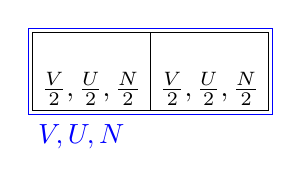
\begin{tikzpicture}
        \coordinate (lu) at (0.45,0.45);
        \coordinate (ro) at (3.55,1.55);
        \coordinate (lu1) at (0.5,0.5);
        \coordinate (lu2) at (2,0.5);
        \coordinate (ro1) at (2,1.5);
        \coordinate (ro2) at (3.5,1.5);
        \draw[blue] (lu) rectangle (ro);
        \draw (lu1) rectangle (ro1);
        \draw (lu2) rectangle (ro2);
        \node[below=8pt, right, blue] at (lu) {$V,U,N$};
        \node[above=8pt, right] at (lu1) {$\frac{V}{2},\frac{U}{2},\frac{N}{2}$};
        \node[above=8pt, right] at (lu2) {$\frac{V}{2},\frac{U}{2},\frac{N}{2}$};
    \end{tikzpicture}
\end{center}
\begin{equation}
    M_{\Delta}^1 \left(\frac{U}{2}\right) = M_{\Delta}^2 \left(\frac{U}{2}\right) \quad \text{und} \quad M_{\Delta} (U) \approx M_{\Delta}^1 \left(\frac{U}{2}\right) \cdot M_{\Delta}^2 \left(\frac{U}{2}\right)
\end{equation}
\begin{equation}
    S(V,U,N) = k \ln(M_{\Delta}(U)) = k \ln\left( M_{\Delta}^1 \left(\frac{U}{2}\right) \right) + k \ln\left( M_{\Delta}^2 \left(\frac{U}{2}\right) \right) = 2 S\left(\frac{V}{2},\frac{U}{2},\frac{N}{2} \right)
\end{equation}
\end{beispiel}

\begin{prop}{Gleichgewicht der Ensemble}
    Im thermodynamischen Limes sind die makroskopischen Eigenschaften von mikrokanonischem, kanonischem und großkanonischem Ensemble äquivalent.
\end{prop}


\subsection{Grundlegende Beziehungen der Thermodynamik}\marginpar{VL 14}
Zustandsgleichungen: Zusammenhang zwischen thermischen Zustandsgößen\\
Beispiel: Zustandsgröße $U\underbrace{(S, \quad V, \quad N)}_{\text{natürliche Zustandsvariablen}}$ ist ein thermisches Potential
\subsubsection{Fundamentalform}
1 HS:
\begin{align}
    dU=\underbrace{\delta Q}_{TdS} + \underbrace{\delta W}_{-pdV+\mu dN}
\end{align}
\begin{definition}{Gibbs'sche Fundamentalform}
    \begin{align}
        dU=TdS-pdV+\mu dN
    \end{align}
\end{definition}
mit den extensiven Größen $U,S,V,N$ und den internsiven Größen $T,p,\mu$\\
Die Zustandsgröße $U=U(S,V,N)$ ist eine thermodynamisches Potential und Funktion der Zustandsvariablen $S,V,N$ (natürliche Variablen)


\subsubsection{Physikalische Notation}
Partielle Ableitungen:
\begin{align}
    \pd{U(S,V,N)}{S}=\left(\pd{U}{S}\right)_{V,N}
\end{align}
Funktionen:
\begin{align}
    U(S,V,N),\overset{\sim}{U}(T,V,N),\overset{\approx}{U}(S,p,N),\overset{\approx}{\overset{\sim}{U}},\overset{\approx}{\overset{\approx}{U}},...
\end{align}
haben völlig verschiedene Abhängigkeiten von Argumenten: trotzdem ein Symbol $U'$!

$\left(\pd{U}{V}\right)_{T,N}$, $\pd{\Tilde{U}(T,V,N)}{V}$ und \underline{nicht} $\pd{U(S,V,N)}{V}$!


\subsubsection{Thermodynamische Kräfte}
$U(S,V,N)$ hat vollständiges Differential
\begin{align}
    dU=\left(\pd{U}{S}\right)_{V,N}dS + \left(\pd{U}{V}\right)_{S,N}dV + \left(\pd{U}{N}\right)_{S,V}dN
\end{align}
Vergleich mit Fundamentalform
\begin{definition}{Thermodynamische Kräfte}
    \begin{align}
        T=\left(\pd{U}{S}\right)_{V,N},\ p=-\left(\pd{U}{V}\right)_{S,N},\ \mu=\left(\pd{U}{N}\right)_{S,V}
    \end{align}
\end{definition}
Analogie zur Mechanik Potential $V(X)$, Kraft $F=-\pd{V}{x}$ wirkt auf $X$. hier th. Potential $U(S,V,N)$, th. Kraft $T=\left(\pd{U}{S}\right)_{V,N}$ wirkt auf S, $p=\left(\pd{U}{V}\right)_{S,N}$ wirkt auf V


\subsubsection{Maxwell Relationen}
\begin{align}
    T(S,V,N)=\left(\pd{U}{S}\right)_{V,N} \hspace{1cm} \text{und} \hspace{1cm} p(S,V,N)= -\left(\pd{U}{V}\right)_{S,N}
\end{align}
Thermodynamische Kräfte:
\begin{itemize}
    \item enthalten einzeln nicht die volle Information von $U$ (da Ableitung)
    \item sind nicht unabhängig, da 2. Ableitung vertauschen
        \begin{align}
            \pdv{U(S,V,N)}{V}{S}=\pdv{U(S,V,N)}{S}{V} &\Rightarrow \text{ Maxwell Relationen} 
        \end{align}
\end{itemize}



\begin{definition}{Maxwell-Relationen}
    \begin{align}
        \left(\pd{T}{V}\right)_{S,N} &= -\left(\pd{p}{S}\right)_{V,N}\\
        \left(\pd{T}{N}\right)_{S,V} &=\left(\pd{\mu}{S}\right)_{V,N}\\
        \left(\pd{\mu}{V}\right)_{S,N} &=-\left(\pd{p}{N}\right)_{S,V}\\
        &\dots
    \end{align}
\end{definition}


\subsubsection{Kalorische und thermische Zustandsgleichung}
Die Funktionen $U(S,V,N),T(S,V,N),p(S,V,N)$ sind schwer experimentell zu bestimmen, da $S$ nicht experimentell einstellbar.\\
Auflösen der Funktion $T(S,V)$ nach $S(T,V)$:
\begin{definition}{kalorische (1) und thermische (2) Zustandsgleichung}
    \begin{align}
        U(S,V) = U(S(T,V),V) \rightarrow U(T,V)\\
        p(S,V) = p(S(T,V),V) \rightarrow p(T,V)
    \end{align}
\end{definition}

\begin{beispiel}{Ideale einatomiges Gas}
    \begin{align}
        U(T,V,N)&=\frac{3}{2}NkT \hspace{1cm} \text{(unabh. von V)}\\
        p(T,V,N)&=\frac{NkT}{V}
    \end{align}
\end{beispiel}

\paragraph{Bemerkung:}
\begin{itemize}
    \item experimentell messbar
    \item enthalten einzeln nicht volle Information
    \item nicht unabhängig
\end{itemize}


\subsubsection{Entropie}
\begin{align}
    S(U,V,N) \; &\widehat{=} \; \text{in der Stat.Physik mikrokan. Ensemble} \\
    dS &= \frac{1}{T}dU + \frac{p}{T}dV-\frac{\mu}{T}dN\\
    &= \left(\pd{S}{U}\right)dU +\left(\pd{S}{V}\right)dV + \left(\pd{S}{N}\right)dN\\
    &\Rightarrow \left(\pd{S}{U}\right)_{V,N}=\frac{1}{T}, \left(\pd{S}{V}\right)_{U,N}=\frac{p}{T},\left(\pd{S}{N}\right)_{U,V}=-\frac{\mu}{T}
\end{align}

\begin{beispiel}{Ideales Gas}
aus stat Physik
    \begin{align}
        S=kN\left(\ln \frac{V}{N\lambda^3} + \frac{5}{2}\right) \quad \text{mit} \quad \lambda=\frac{h}{\sqrt{4\pi m U/(3N)}}
    \end{align}
    \begin{align}
        \frac{p}{T} &=\left(\pd{S}{V}\right)_{U,N}=kN\frac{1}{V} \quad \Rightarrow p=\frac{kNT}{V} \quad \checkmark\\
        \frac{1}{T} &=\left(\pd{S}{U}\right)_{V,N}=kN\frac{3}{2}\frac{1}{U} \quad \Rightarrow U=\frac{3}{2}kNT \quad \checkmark
    \end{align}
\end{beispiel}


\subsubsection{Euler-Gleichung, Gibbs-Duhen Relation}
Nutze Extensivität der inneren Energie (gilt nur für kurzreichweitige WW)
\begin{align}
    U(\lambda S,\lambda V, \lambda N)&=\lambda U(S,V,N)\\
    \eval{\dv{\lambda}}_{\lambda=1}&: \eval{\pd{U(S,V,N)}{S}}_{\lambda S,\lambda V,\lambda N, \lambda=1}S\\
    &= \underbrace{\left(\pd{U}{S}\right)_{V,N}}_{T} S+ \underbrace{\left(\pd{U}{V}\right)_{S,N}}_{-p} V + \underbrace{\left(\pd{U}{N}\right)_{S,V}}_{\mu} N = U(S,V,N)
\end{align}

\begin{definition}{Euler-Gleichung}
    \begin{align}
        U=TS-pV+\mu N
    \end{align}
    Differentielle Form
    \begin{align}
        dU=TdS + SdT - pdV - Vdp + \mu dN + Nd\mu
    \end{align}
    
\end{definition}
Subtraktion der Fundamentalform:
    \begin{align}
        dU = TdS -pdV + \mu dN
    \end{align}
\begin{definition}{Gibbs-Duhen-Relation}
    \begin{align}
        0= SdT - Vdp + Nd\mu
    \end{align}
\end{definition}
mit extensiven Größen $S,V,N$ und intensiven Größen $T,p,\mu$ $\leftarrow$ können nicht unabhängig voneinander variiert werden.


\subsection{Zustandsänderung und Materialgrößen}
\paragraph{Zustandsänderung (N=const)}
\begin{itemize}
    \item isotherm: $T=const$
    \item isochor: $V=const$
    \item isobar: $p=const$
    \item adiabatisch: $S=const,\delta Q = 0$
    \item quasistatisch : so langsam, das System immer im (partiellen) Gleichgewicht
    \item reversibel: $\Delta S_{Gesamt}=0$ (umkehrbar, hypothetischer Grenzfall, mind. quasistatisch)
\end{itemize}
\begin{beispiel}{quasistatisch (aber nicht reversibel)}
    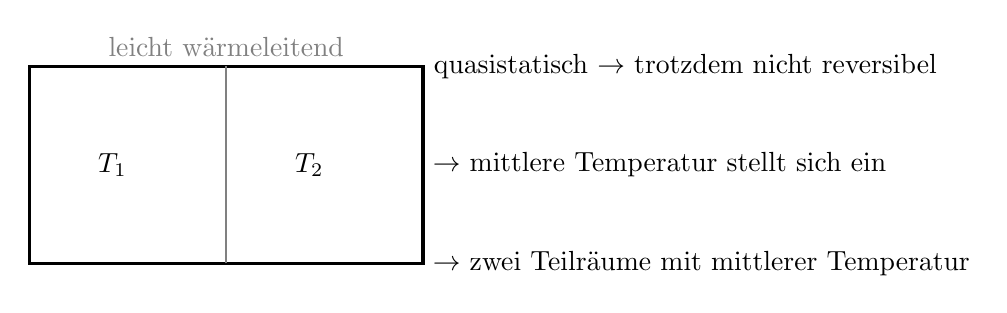
\begin{tikzpicture}[scale=0.5]
        \draw[very thick] (0,0) rectangle (10,5) node[anchor=west]{quasistatisch $\rightarrow$ trotzdem nicht reversibel};
        \draw[thick, black!50] (5,0) -- (5,5) node[anchor=south]{leicht wärmeleitend};
        \draw (10,2.5) node[anchor=west]{$\rightarrow$ mittlere Temperatur stellt sich ein};
        \draw (10,0) node[anchor=west]{$\rightarrow$ zwei Teilräume mit mittlerer Temperatur};
        \draw (1.5,2.5) node[anchor=west]{$T_1$};
        \draw (6.5,2.5) node[anchor=west]{$T_2$};
    \end{tikzpicture}
\end{beispiel}

\paragraph{Materialgößen}
\begin{itemize}
    \item Wärmekapazität bei konst Volumen
        \begin{align}
            c_v = \eval{\frac{\delta Q}{dT}}_V \overset{\delta Q=TdS}{=} T\left(\pd{S}{T}\right)_{V} \overset{\delta Q = dU + pdV}{=} \left(\pd{U}{T}\right)_{V}
        \end{align}
    \item Wärmekap. bei konst Druck
        \begin{align}
            c_p = \eval{\frac{\delta Q}{dT}}_p = T\left(\pd{S}{T}\right)_{p} = \left(\pd{U}{Tf}\right)_{p} + p\left(\pd{V}{T}\right)_{p}
        \end{align}
    \item isobarer (sogn. thermischer) Ausdehnungskoeffizient
    \begin{equation}
        \alpha = \frac{1}{V} \cdot \left( \pd{V}{T}\right)_p
    \end{equation}
    \item isochorer Spannungskoeffizient
    \begin{equation}
        \sigma = \frac{1}{p} \cdot \left(\pd{p}{T}\right)_V
    \end{equation}
    \item isotherme Kompressibilität
    \begin{equation}
        \kappa_T = - \frac{1}{V}\cdot \left(\pd{V}{p}\right)_T
    \end{equation}
    \item adiabatische Kompressibilität
    \begin{equation}
        \kappa_S = - \frac{1}{V} \cdot \left(\pd{V}{p}\right)_S
    \end{equation}

\end{itemize}

\newpage 
\subsection{Thermodynamische Potentiale}\marginpar{VL 15}
\subsubsection{Eigenschaften}
\begin{itemize}
    \item Zustandsgrößen mit Einheit Energie, insb. $U(S,V,N)$
    \item minimal im Gleichgewicht
    \item Abhängigkeit von natürlichen Zustandsvariablen
    \item partielle Ableitungen nach Zustandsvariablen sind einfache Ausdrücke
    \begin{itemize}
    \item[$\rightarrow$] thermodynamische Kräfte
    \end{itemize}
    \item volle thermodynamische Information
    \item alle 5 Potentiale sind gleichwertig, je nach physikalischer/chemischer Situation einfacher
\end{itemize}

\paragraph{Bemerkung} Entropie $S(U,V,N)$ ist thermodynamisches Potential im weiteren Sinne:
\begin{itemize}
    \item Einheit einer Entropie ($k_B$)
    \item maximal im Gleichgewicht
    \item partielle Ableitungen etwas komplizierter, z.B. $\left(\pd{S}{V}\right)_{U,N} = \frac{p}{T}$
\end{itemize}

\subsubsection{Freie Energie}
System mit festem $V,N$ in Umgebung mit $T$ \\
Ziel: Funktion von $T,V,N$ ($\widehat{=}$ kanonisches Ensemble mit $\beta = \frac{1}{kT}$)

\paragraph{Legendre-Transformation}

Funktion $f(x,t) \quad \rightarrow$ Ersetze $x$ durch $y$, $t$ unverändert; falls:
\begin{equation}
    y = \pdv{f(x,t)}{x} \quad \text{ und $f$ konvex } \frac{\partial^2 f(x,t)}{\partial x^2} > 0
\end{equation}
$y$ heißt konjugiert zu $x$ bezüglich $f$
\begin{equation}
    \rightarrow \text{Legendre-Transformierte  } \quad g(y,t):= f(x,t) - xy
\end{equation}
Eigenschaften:
\begin{itemize}
    \item hängt nur von $y,t$ ab, nicht von $x$
    \begin{equation}
        \frac{d}{dx} g(y,t) = \underbrace{\pdv{f(x,t)}{x}}_{=y} -y = 0 \quad \checkmark
    \end{equation}
    \item kein Informationsverlust
    \begin{proof}
        Rückkehr zu $f(x,t)$. Was ist $x$? $\pdv{g(y,t)}{y} = -x$ Nun machen wir die inverse Legendre-Transformation: $f(x,t) = g(y,t) + xy$
    \end{proof}
\end{itemize}

\subparagraph{Beispiel} klassische Mechanik
\begin{itemize}
    \item[] Lagrange-Funktion $L(q,\Dot{q})$ mit $p = \pdv{L}{\Dot{q}}$
    \item[$\Rightarrow$] Hamilton-Funktion: $-H(q,p) = L(q,\Dot{q}) - \Dot{q}p$ 
\end{itemize}
Anwendung auf thermodynamisches Potential $U(S,V,N)$
\begin{equation}
    T = \text{konj. Variable zu } S, \text{ da } T = \pdv{U}{S}
\end{equation}
Legendre-Transformation:
\begin{definition}{Freie Energie / Helmholtz-Potential}
\begin{equation}
    F(T,V,N) := U(S,V,N) - T \cdot S
\end{equation}
\end{definition}
\textbf{Bemerkung:}
\begin{itemize}
    \item hängt nicht von $S$ ab $\checkmark$
    \item volle thermodynamische Information enthalten
\end{itemize}


\subsubsection{Übersicht der thermodynamischen Potentiale}
natürliche Variablenpaare: $S \leftrightarrow T$, $V \leftrightarrow p$, $N \leftrightarrow \mu$

\begin{table}[h]
    \centering
    \caption{Übersicht zu den thermodynamischen Potentialen}
    \begin{tabular}{lcll}
         1 & $(S,V,N)$ & $U$ & innere Energie\\
         2 & $(T,V,N)$ & $F:= U - TS$ & freie Energie \\
         3 & $(S,p,N)$ & $H:= U + pV$ & Enthalpie \\
         4 & $(T,p,N)$ & $G := U - TS +pV$ & freie Enthalpie \\
         5 & $(S,V,\mu)$ & Teilchenaustausch + feste Entropie & $\rightarrow$ keine Anwendung\\
         6 & $(T,V,\mu)$ & $\Phi := U - TS - \mu N$ & großkanonisches Potential\\
         7 & $(S,p,\mu)$ & Teilchenaustausch + feste Entropie & $\rightarrow$ keine Anwendung\\
         8 & $(T,p,\mu)$ & $\Psi := U - TS + pV - \mu N = 0$ & $\rightarrow$ Euler-Gleichung\\
    \end{tabular}
    \label{tab:thermodynamische Potentiale}
\end{table}

\paragraph{Bemerkung:}
Nutze die Euler-Gleichung: $U = TS-pV+\mu N$, um Potentiale zu vereinfachen:
\begin{align}
    G(T,p,N) &= \mu N = \mu(T,p,N) \stackrel{\text{Extensivität}}{=} \mu(T,p) N \\
    \Phi(T,V,\mu) &= - pV \stackrel{\text{Extensivität}}{=} - p(T,\mu) V
\end{align}

\subsubsection{Beispiele für physikalische/chemische Situationen}
\begin{itemize}
    \item[U:] isoliertes System
    \item[F:] System im Wärmebad $T$
    \item[H:] chemische Reaktion bei konstantem Druck $p$
    \item[G:] chemische Reaktion bei konstantem $p$ und $T$
    \item[$\Phi$:] Adsorption an Oberflächen / Elektronengas in Metall 
\end{itemize}

\subsubsection{Differentielle Form}
\begin{align}
    \text{Fundamentalform} \quad dU &= T \cdot dS - p\cdot dV + \mu \cdot dN\\
    dF = dU - T \cdot dS - S \cdot dT \quad dF &= -S \cdot dT - p\cdot dV + \mu \cdot dN\\
    dH &= T \cdot dS + V\cdot dp + \mu \cdot dN \\
    dG &= -S \cdot dT + V \cdot dp + \mu \cdot dN \\
    d\Phi &= -S \cdot dT - p\cdot dV - N \cdot d\mu
\end{align}
    
\subsubsection{Thermodynamische Kräfte}
\begin{align}
    \left(\pdv{U}{S}\right)_{V,N} &= T, \quad \left(\pdv{U}{V}\right)_{S,N} = -p, \quad \left(\pdv{U}{N}\right)_{S,V} = \mu \\
    \left(\pdv{F}{T}\right)_{V,N} &= -S, \quad \left(\pdv{F}{V}\right)_{T,N} = -p, \quad \left(\pdv{F}{N}\right)_{T,V} = \mu \\
    \left(\pdv{H}{S}\right)_{p,N} &= T, \quad \left(\pdv{H}{p}\right)_{S,N} = V, \quad \left(\pdv{H}{N}\right)_{S,p} = \mu \\
    \left(\pdv{G}{T}\right)_{p,N} &= -S, \quad \left(\pdv{G}{p}\right)_{T,N} = V, \quad \left(\pdv{G}{N}\right)_{T,p} = \mu \\
    \left(\pdv{\Phi}{T}\right)_{V,\mu} &= -S, \quad \left(\pdv{\Phi}{V}\right)_{T,\mu} = -p, \quad \left(\pdv{\Phi}{\mu}\right)_{T,V} = -N
\end{align}

\subsubsection{Maxwell Relationen}
\begin{align}
    \frac{\partial^2 U(S,V,N)}{\partial V \partial S} &=\frac{\partial^2 U(S,V,N)}{\partial S\partial V} \Rightarrow \left(\pdv{T}{V}\right)_{S,N} = - \left(\pdv{p}{S}\right)_{V,N}\\
    \partial_{SN}^2 &= \partial_{NS}^2, \quad \partial_{VN}^2 = \partial_{NV}^2, \quad ...\\
    \frac{\partial^2 F(T,V,N)}{\partial V \partial T} &=\frac{\partial^2 F(T,V,N)}{\partial T\partial V} \Rightarrow -\left(\pdv{S}{V}\right)_{T,N} = - \left(\pdv{p}{T}\right)_{V,N}\\
    \partial_{TN}^2 &= \partial_{NT}^2, \quad \partial_{VN}^2 = \partial_{NV}^2, \quad ...
\end{align}

\subsubsection{Thermodynamisches Viereck (N=const)}
\textbf{Variablenpaare:} $S \leftrightarrow T$ und $V \leftrightarrow p$ \textbf{Potentiale:} $U,F,G,H$
\begin{center}
\begin{tikzpicture}[
roundnode/.style={circle, draw=blue!60, fill=blue!5, very thick, minimum size=7mm},
]
%Nodes
\node[roundnode]      (S)                    {S};
\node[roundnode]      (U)       [right=of S] {U};
\node[roundnode]      (V)       [right=of U] {V};
\node[roundnode]      (F)       [below=of V] {F};
\node[roundnode]      (T)       [below=of F] {T};
\node[roundnode]      (H)       [below=of S] {H};
\node[roundnode]      (p)       [below=of H] {p};
\node[roundnode]      (G)       [right=of p] {G};


%Lines
\draw[->,very thick] (S.south east) -- (T.north west);
\draw[->,very thick] (p.north east) -- (V.south west);
\end{tikzpicture}
\end{center}
\paragraph{Merkregel}
\begin{quote}
    dt.:  \underline{S}\underline{U}\underline{V} \underline{H}ilft \underline{F}ysikerinnen \underline{p}ei \underline{G}roßen \underline{T}aten.
\end{quote}
\begin{quote}
    engl.: \underline{G}ood \underline{p}hysicists \underline{H}ave \underline{S}tudied \underline{U}nder \underline{V}ery \underline{F}ine \underline{T}eachers.
\end{quote}
\paragraph{Beispiel}
$\Longrightarrow$ mit Potential anfangen, zur ableitenden Variable gehen und von dort dem Pfeil folgen, Pfeilrichtung ergibt Vorzeichen
\begin{align}
    \pdv{H}{S} &= T  \qquad \pdv{G}{p} = V\\
    \pdv{G}{T} &= -S \qquad \pdv{F}{V} = -p
\end{align}

\subsubsection{Verbindung zur statistischen Physik}
\paragraph{kanonisches Ensemble} (passt zur freien Energie $F$)
\begin{itemize}
    \item[] Dichteoperator:
    \begin{equation}
        \varrho = \frac{1}{Z} e^{-\beta H(V,N)} \quad \text{mit} \quad Z(\beta,V,N) = \trace\left(e^{-\beta H(V,N)}\right)
    \end{equation}
    \item[] Entropie:
    \begin{align}
        S(\beta,V,N) &= -k \trace(\varrho \ln(\varrho)) = k \ln(Z) + \underbrace{k \beta}_{\frac{1}{T}} \underbrace{\langle H \rangle}_{U}\\
        &\Rightarrow F = U-TS = -k T \ln(Z) \\
        &\fcolorbox{red}{white}{$\underbrace{F(T,V,N)}_{\text{Thermodyn.}} = \underbrace{-k T \ln\left(Z\left(\frac{1}{kT},V,N\right)\right)}_{\text{stat. Physik}}$}
    \end{align}
\end{itemize}

\paragraph{großkanonisches Ensemble}
\begin{equation}
    \fcolorbox{red}{white}{$\Phi(T,V,\mu) = -k T \ln\left(Z_G\left(\frac{1}{kT},V,\mu\right)\right)$}
\end{equation}

\paragraph{mikrokanonisches Ensemble}
\begin{equation}
    \fcolorbox{red}{white}{$S(U,V,N) = k \ln\left(Z_{mikro}(U,V,N)\right)$}
\end{equation}


\subsection{Stabilitätsbedingungen}\marginpar{VL 16}
\begin{itemize}
    \item thermische Stabilität:
    \begin{equation}
        c_V = \left(\pdv{U}{T}\right)_{V,N} > 0
    \end{equation}
    \item mechanische Stabilität:
    \begin{equation}
        \kappa_T = - \frac{1}{V} \left(\pdv{V}{p}\right)_{T,N} > 0
    \end{equation}
    \item chemische Stabilität:
    \begin{equation}
        \left(\pdv{N}{\mu}\right)_{T,V} > 0
    \end{equation}
\end{itemize}

\subsection{Phasengleichgewichte}
\begin{itemize}
    \item[] Stoff kann in verschiedenen Phasen auftreten (fest, flüssig, gasförmig) mit verschiedenen Eigenschaften (Dichte, Kompressibilität)
    \item[] Phasengleichgewicht: zwei oder mehr Phasen in Berührung und im Gleichgewicht
    \begin{itemize}
        \item[z.B.:] Eis + Wasserdampf + Wasser
        \item[] (inhomogenes System mit drei homogenen Teilsystemen)
    \end{itemize}
\end{itemize}

\paragraph{2 Phasen}
\begin{align}
    T_1 = T_2, \quad p_1 = p_2, \quad \mu_1 = \mu_2 \quad \Rightarrow \quad \mu_1(p,T) = \mu_2(p,T) \quad (\text{nur noch 1 Größe variabel})\\
    \Longrightarrow \text{ Koexistenzkurve (z.B. flüssig / gasförmig)}
\end{align}
\begin{center}
    \begin{tikzpicture}[scale=0.9]
        \begin{axis}[
        axis lines = left,
        axis line style={my axis},
        xmin=0, xmax = 6,
        ymin=0, ymax = 3.5,
        xtick=\empty, ytick=\empty,]
        \addplot[domain=1:5, samples=100, color=blue,]{exp(x/4)-0.5};
    \end{axis}
    \draw (7,0) node[anchor=west]{$T$};
    \draw (0,5.5) node[anchor=east]{$p$};
    \draw (5,4) node[anchor=west]{$\rightarrow$ Dampfdruckkurve};
    \draw[black!40] (3.5,2.5) node[anchor=west]{gasförmig};
    \draw[black!40] (2,3) node[anchor=west]{flüssig};
    \end{tikzpicture}
\end{center}

\paragraph{3 Phasen}
\begin{align}
    \mu_1(p,T) = \mu_2(p,T) = \mu_3(p,T) \\
    \Longrightarrow \text{ Tripelpunkt}\\
    (H_2O: \SI{0.01}{\celsius}, \SI{600}{\pascal})
\end{align}
\begin{center}
    \begin{tikzpicture}[scale=0.9]
        \begin{axis}[
        axis lines = left,
        axis line style={my axis},
        xmin=-1, xmax = 6,
        ymin=0, ymax = 3.5,
        xtick=\empty, ytick=\empty,]
        \addplot[domain=1:4.5, samples=100, color=blue,]{exp(x/4)-0.24};
        \addplot[domain=0:1, samples=100, color=green,]{1/x};
        \addplot[domain=-0.5:1, samples=100,]{exp(x/2)-0.6};
    \end{axis}
    \draw (7,0) node[anchor=west]{$T$};
    \draw (0,5.5) node[anchor=east]{$p$};
    \draw[blue] (5,4) node[anchor=west]{$\rightarrow$ Dampfdruckkurve};
    \draw (1,0.5) node[anchor=west]{$\rightarrow$ Sublimationsdruckkurve};
    \draw[green] (1.5,5.5) node[anchor=west]{$\rightarrow$ Schmelzdruckkurve};
    \draw[black!40] (4.5,2.5) node[anchor=west]{gasförmig};
    \draw[black!40] (2,4) node[anchor=west]{flüssig};
    \draw[black!40] (0,2) node[anchor=west]{fest};
    \filldraw[red] (1.95,1.7) circle (3pt) node[anchor=north west]{Tripelpunkt};
    \end{tikzpicture}
\end{center}

\subsubsection{Clausius-Clapeyron-Gleichung}
2 Phasen im Gleichgewicht
\begin{align}
    &\Rightarrow d\mu_1(p,T) = d\mu_2(p,T)\\
    \text{Gibbs-Duhem: } \quad &S dT - V dp + N d\mu = 0\\
    &\Rightarrow d\mu = - \underbrace{\frac{S}{N}}_{=: s} + \underbrace{\frac{V}{N}}_{=:v}\\
    &\Rightarrow -s_1 dT + v_1 dp = -s_2 dT + v_2 dp\\
    &\Rightarrow (s_2 -s_1) dT = (v_2 - v_1) dp\\
    &\text{mit: } q_{1\to2} = T (s_2-s_1) \\
    &\Longrightarrow \quad \fcolorbox{red}{white}{\Large$\frac{dp}{dT}= \frac{(s_2-s_1)}{(v_2 - v_1)} = \frac{q_{1\to2}}{T(v_2-v_1)}$} \quad \text{(Clausius Clapeyron)}
\end{align}

\begin{itemize}
    \item[$q_{1\to 2}$]: Wärme pro Teilchen, die bei Phasenumwandlung von 1 nach 2 zugeführt werden muss
    \item[] flüssig $\rightarrow$ gasförmig: Verdampfungswärme
    \item[] fest $\rightarrow$ flüssig: Schmelzwärme
    \item[] fest $\rightarrow$ gasförmig: Sublimationswärme
    \item[$\rightarrow$] latente (\enquote{versteckte}) Wärme
\end{itemize}

\paragraph{Beispiele}
\begin{itemize}
    \item Dampfdruckkurve:
    \begin{align}
        v_g &> v_f \quad \Rightarrow \quad \frac{dp}{dT} = \frac{q_{1\to2}}{T\cdot v_g} \\
        \text{ideales Gas: } pV &= NkT \quad \Rightarrow \quad v_g = \frac{V}{N} = \frac{kT}{p}\\
        \rightarrow \frac{dp}{dT} &= \frac{p}{T^2} \frac{q_{fl\to g}}{k}\\
        &\stackrel{TdV}{\Longrightarrow} \frac{dp}{p} = \frac{q_{fl\to g}}{k} \ \frac{dT}{T^2} \Rightarrow \quad \text{Annahme: $q_{fl \to g}$ nicht von $T$ abhängig}\\
        &\Rightarrow \ln(p)\Big\vert_{p_0}^p = \frac{q_{fl\to g}}{k} \left(-\frac{1}{T}\right)\Big\vert_{T_0}^T\\
        &\Rightarrow p(T) = p_0 \cdot e^{-\frac{q_{fl\to g}}{k}\left(\frac{1}{T}-\frac{1}{T_0}\right)}
    \end{align}
    \item Sublimationsdruckkurve:
    \begin{align}
        v_g \gg v_f \quad &\Rightarrow \quad \text{wie Dampfdruckkurve}\\
        &\rightarrow q_{fest\to g} > q_{fl \to g} \quad \Rightarrow \quad \frac{dp}{dT} \text{ steiler}
    \end{align}
    \begin{center}
    \begin{tikzpicture}[scale=0.4]
        \begin{axis}[
        axis lines = left,
        axis line style={my axis},
        xmin=-1, xmax = 6,
        ymin=0, ymax = 3.5,
        xtick=\empty, ytick=\empty,]
        \addplot[domain=1:4.5, samples=100,]{exp(x/4)-0.24};
        \addplot[domain=0:1, samples=100,]{1/x};
        \addplot[domain=-0.5:1, samples=100,]{exp(x/2)-0.6};
        \addplot[domain=0:3, samples=100, color=red,]{sqrt(x^3-1)+0.75};
    \end{axis}
    \draw (7,0) node[anchor=west]{$T$};
    \draw (0,5.5) node[anchor=east]{$p$};
    \draw[black!40] (4.5,2) node[anchor=west]{gasf};
    \draw[black!40] (3,4) node[anchor=west]{fl};
    \draw[black!40] (-0.3,2) node[anchor=west]{fest};
    \draw[red] (2.8,5) node[anchor=west]{$CO_2$};
    \filldraw (1.95,1.7) circle (3pt);
    \end{tikzpicture}
\end{center}
    \item Schmelzdruckkurve:
    \begin{align}
        v_{fest} \approx v_{fl} \quad &\Rightarrow \quad \frac{dp}{dt} \text{ ist sehr steil}\\
        \text{Wasser: } v_{fest} > v_{fl} \quad &\Rightarrow \quad \frac{dp}{dT} < 0\\
        \text{meist: } v_{fest} < v_{fl} \quad &\Rightarrow \quad \frac{dp}{dT} > 0\\
    \end{align}
\end{itemize}

\subsubsection{Phasenregel von Gibbs}
$K$ (Komponenten) verschiedene Stoffe jeweils in $P$ verschiedenen Phasen (fest, flüssig, gasförmig) im Gleichgewicht $\longrightarrow$ Wieviele Freiheitsgrade gibt es? bzw. Was ist de Zahl unabhängiger intensiver Variablen?
\begin{equation}
    \fcolorbox{red}{white}{\large F = 2 + K - P} \quad \text{Gibbs´sche Phasenregel}
\end{equation}

\paragraph{Beweis:} intensive Variablen: $T, \,p,$ Konzentrationen $\frac{N_k^i}{N^i}$ mit $N_k^i$ -k-te Komponente in Phase i und $N^i$ - Teilchen in Phase i
\begin{equation}
    \Longrightarrow 2 + K\cdot P \quad \text{ intensive Variablen}
\end{equation}
\begin{itemize}
    \item Abhängigkeiten
    \begin{itemize}
        \item alle Phasen $i = 1,...,P$:
        \begin{equation}
            \sum_{k=1}^K \frac{N_k^i}{N^i} = \frac{N^i}{N^i} = 1 \quad \Rightarrow \text{ P Abhängigkeiten}
        \end{equation}
        \item alle Komponenten $k = 1,...,K$
        \begin{equation}
            \mu_k^1 = \mu_k^2 = ... = \mu_k^P \quad \Rightarrow \quad (P-1) \cdot K \text{ Gleichungen}
        \end{equation}
        \begin{equation}
            \Rightarrow F = 2 + K\cdot P - (P + (P-1)\cdot K) = 2 + K - P \quad \checkmark
        \end{equation}
    \end{itemize}
\end{itemize}

\subparagraph{Beispiele:}
\begin{itemize}
    \item Wasser + Wasserdampf: $K=1$, $P=2$ $\Rightarrow \quad F=1 \quad \Rightarrow$ Dampfdruckkurve
    \item Tripelpunkt: $F=0$
\end{itemize}

\subsubsection{Van der Waals-Gas}
\begin{equation}
    \left(p+a\frac{N^2}{V^2}\right) \left(V-Nb\right) = NkT
\end{equation}
Korrektur der Zustandgleichung des idealen Gases aufgrund von Wechselwirkungen (beschreibt Phasenübergang flüssig $\rightarrow$ gasförmig $\widehat{=}$ Dampfdruckkurve)
\begin{itemize}
    \item[$Nb$] Volumen wird durch Eigenvolumen anderer Gasteilchen reduziert ($\propto N$)
    \item[$a\frac{N^2}{V^2}$] Druck wird erhöht durch Binnendruck anziehender Kräfte (Randteilchen werden nach innen gezogen $\rightarrow$ hoher Druck; $\frac{N}{V}$ im Volumen und $\frac{N}{V}$ an der Oberfläche)
\end{itemize}
$a, \, b > 0$ teilchenspezifische Parameter
\begin{equation}
    p(V,T) = \frac{NkT}{V-Nb} - a \frac{N^2}{V^2} \quad \Rightarrow \quad p(v,T) = \frac{kT}{v-b} - a \frac{1}{v^2}
\end{equation}
Isothermen im $p-V-$Diagramm:

\begin{center}
    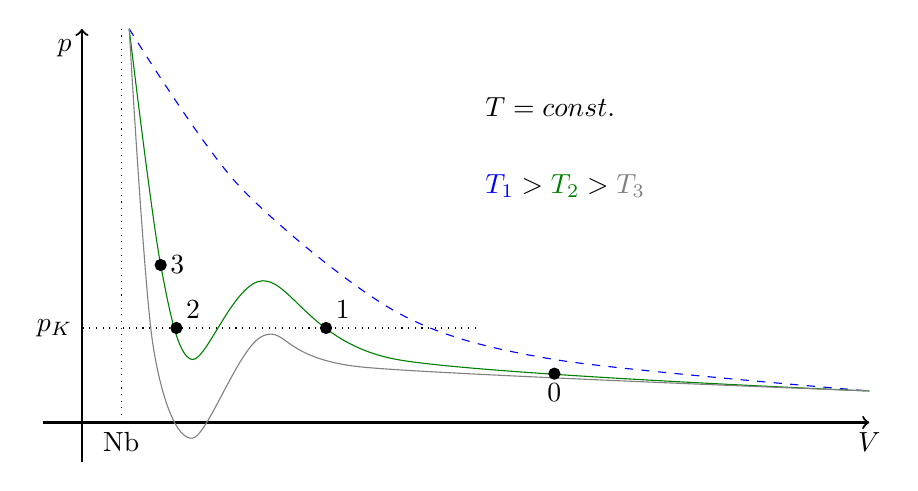
\begin{tikzpicture}
        \draw[->,thick] (-0.5,0) -- (10,0) node[anchor=north]{$V$};
        \draw[->,thick] (0,-0.5) -- (0,5) node[anchor=north east]{$p$};
        \draw[dotted] (0.5,5) -- (0.5,0) node[anchor=north]{Nb};
        \coordinate (a) at (0.6,5);
        \coordinate (b) at (10,0.4);
        \draw[dashed, blue] plot [smooth] coordinates {(a) (2,3)  (4,1.4) (6,0.8) (b)};
        \draw[green!50!black] plot [smooth] coordinates{(a) (1,2) (1.4,0.8) (2.3,1.8) (4,0.8) (b)};
        \draw[black!50] plot [smooth] coordinates{(a) (0.9,1) (1.4,-0.2) (2.3,1.1) (3.6,0.7) (b)};
        \draw (5,4) node[anchor=west]{$T=const.$};
        \draw (5,3) node[anchor=west]{$\color{blue} T_1 \color{black} > \color{green!50!black} T_2 \color{black} > \color{black!50} T_3$};
        \filldraw (1,2) circle (2pt) node[anchor=west]{3};
        \filldraw (1.2,1.2) circle (2pt) node[anchor=south west]{2};
        \filldraw (3.1,1.2) circle (2pt) node[anchor=south west]{1};
        \filldraw (6,0.62) circle (2pt) node[anchor=north]{0};
        \draw[dotted] (5,1.2) -- (0,1.2) node[anchor=east]{$p_K$};
    \end{tikzpicture}
\end{center}

\paragraph{Bemerkungen:}
\begin{itemize}
    \item $p < 0$ nicht sinnvoll
    \item mechanische Stabilität:
    \begin{align}
        \left(\pdv{p}{V}\right)_{T,N} < 0 \quad \rightarrow \quad \text{nicht sinnvoll}
    \end{align}
    \item bei $T$, $p$ fest $\rightarrow$ Welches Volumen $V$?
    \item[$\rightarrow$] 3 Schnittpunkte, aber nur 2 sinnvoll
    \item Kompression bei $T=const.$
    \begin{itemize}
        \item[0:] Gas 
        \item[1:] Beginn Verflüssigung
        \item[$\rightarrow$] Koexsistenz von Gas und Flüssigkeit
        \begin{equation}
            p_1 = p_2 \qquad T_1 = T_2 \qquad \mu_1 = \mu_2 \qquad (p=const.)
        \end{equation}
        \item[2:] Verflüssigung vollständig
        \item[3:] Flüssigkeit
        \begin{itemize}
            \item[$\longrightarrow$] \textbf{Wo liegt Koexsitenzgerade $p_k$?}
        \end{itemize}
         
    \end{itemize}
\end{itemize}


\subsubsection*{Maxwell-Konstruktion des Koexistenzbereiches}\marginpar{VL 17}
$\rightarrow$ Freie Energie $F(T,V)$ Zustandsgröße $\Rightarrow$ wegunabhängig!
\begin{align}
    F_2-F_1 &= \underbrace{\int_1^2 \ }_{\text{v.d.W.}} dF = \underbrace{\int_1^2 \ }_{p=p_k=const.} dF \\
    dF &= -S \ dT - p \ dV \stackrel{T=const.}{=} -p \ dV \\
    \underbrace{\overbrace{\int_1^2 \ }^{\text{v.d.W.}} dF}_{\text{Fläche unter v.d.W. Kurve}} &= \underbrace{p_k \cdot (V_2-V_1)}_{\text{rechteckige Fläche}}
\end{align}

 $\Rightarrow$ Wert muss so gewählt werden, dass die rote und grüne Flächen null ergeben müssen. 
 \begin{center}
 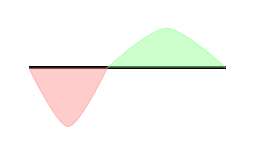
\begin{tikzpicture}[scale=0.5]
     \draw[thick] (0,0) -- (5,0);
     \filldraw[red!40, semitransparent] plot [smooth] coordinates {(0,0) (1,-1.5) (2,0)};
     \filldraw[green!40, semitransparent] plot [smooth] coordinates{(2,0) (3.5,1) (5,0)};
 \end{tikzpicture}
 \end{center}


\begin{align}
    \pdv{p(T,V)}{V} = 0 \quad &, \quad \pdv[2]{p(T,V)}{V}=0\\
    &\Longrightarrow p_k, \ T_k, \ V_k
\end{align}

\begin{center}
    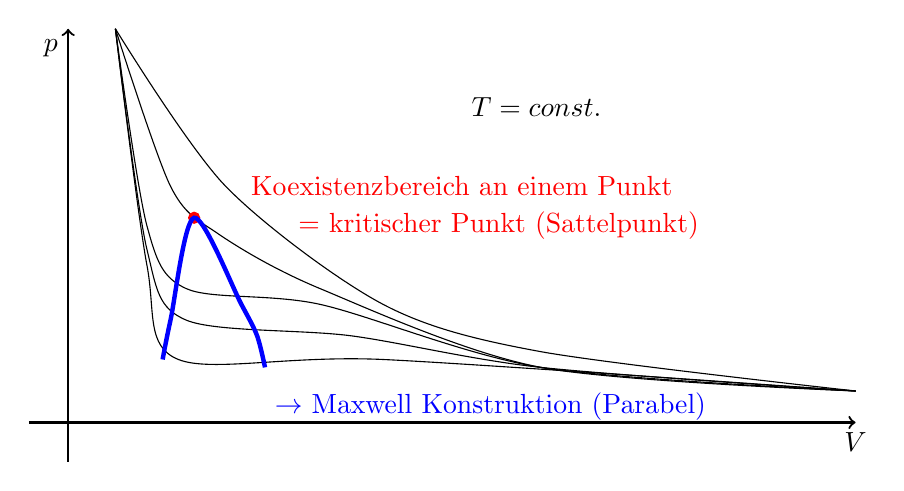
\begin{tikzpicture}
        \draw[->,thick] (-0.5,0) -- (10,0) node[anchor=north]{$V$};
        \draw[->,thick] (0,-0.5) -- (0,5) node[anchor=north east]{$p$};
        \coordinate (a) at (0.6,5);
        \coordinate (b) at (10,0.4);
        \draw plot [smooth] coordinates {(a) (2,3)  (4,1.5) (6,0.9) (b)};
        \draw plot [smooth] coordinates{(a) (1,2) (1.4,0.8) (4,0.8) (b)};
        \draw plot [smooth] coordinates{(a) (1,2.2) (1.5,1.3)(3.6,1.1) (6,0.7) (b)};
        \draw plot [smooth] coordinates{(a) (1,2.5) (1.5,1.7)(3.2,1.5) (6,0.7) (b)};
        \draw plot [smooth] coordinates{(a) (1.3,3) (1.9,2.4)(3.2,1.7) (6,0.7) (b)};
        \draw (5,4) node[anchor=west]{$T=const.$};
        \filldraw[red] (1.6,2.6) circle (2pt);
        \draw[red] (2.2,3) node[anchor=west]{Koexistenzbereich an einem Punkt};
        \draw[ultra thick,blue] plot [smooth] coordinates{(1.2,0.8) (1.3,1.3) (1.6,2.6) (2.2,1.5) (2.4,1.1) (2.5,0.7)};
        \draw[red] (2.8,2.5) node[anchor=west]{= kritischer Punkt (Sattelpunkt)};
        \draw[blue](2.5,0.2) node[anchor=west]{$\rightarrow$ Maxwell Konstruktion (Parabel)};
    \end{tikzpicture}
    \begin{tikzpicture}[scale=0.9]
        \begin{axis}[
        axis lines = left,
        axis line style={my axis},
        xmin=0, xmax = 6,
        ymin=0, ymax = 3.5,
        xtick=\empty, ytick=\empty,]
        \addplot[domain=1:5, samples=100, color=blue,]{exp(x/4)-0.5};
    \end{axis}
    \draw (7,0) node[anchor=west]{$T$};
    \draw (0,5.5) node[anchor=east]{$p$};
    \filldraw[red] (5.7,4.8) circle (3pt)  node[anchor=west]{kritischer Punkt};
    \draw (6,4) node[anchor=west]{$\rightarrow$ darüber kein Phasenübergang mehr};
    \draw[black!40] (3.5,2.5) node[anchor=west]{gasförmig};
    \draw[black!40] (2,3) node[anchor=west]{flüssig};
    \draw (6,2) node[anchor=west]{$\rightarrow$ Stehenbleiben an Dampfdruckkurve};
    \draw (6.5,1.2) node[anchor=west]{$\widehat{=}$ Koexistenzgerade};
    \end{tikzpicture}
\end{center}

\paragraph{Bemerkungen:}
\begin{itemize}
    \item Für $T>T_k$ sind Flüssigkeit und Gas nicht unterscheidbar
    \item Phasenübergang 1.Ordnung: Durchgang durch Dampfdruckkurve (z.B. $T=const$, und $p$ varriert)
    \begin{itemize}
        \item z.B. $T=const.$ und $p$ variiert
        \item $V_{fl} \neq V_{gas}$ ; $V(p)=\left(\pdv{G}{p}\right)_{T,N}$
        \item 1.Ordnung, da $V(p)$ unstetig
        \item Umwandlungswärme
    \end{itemize}
    \item Phasenübergang 2.Ordnung: kritischer Punkt (z.B. $\Delta V = V_{gas}-V_{fl}$ als Funktion von $T$)
    \begin{itemize}
        \item bei $T>T_k: \ \Delta V = 0$\\
        bei $T<T_k: \ \Delta V > 0$ mit $\lim_{T\rightarrow T_k} \Delta V = 0$
        \item 2. Ordnung, da $\Delta V(T)$ stetig, kontinuierlicher Phasenübergang
        \item keine Umwandlungswärme
    \end{itemize}
\end{itemize}


\subsubsection{Osmotischer Druck}
\begin{definition}{Halbdurchlässige Membran}
    Lösungsmittel geht durch, gelöster Stoff nicht\\
    Beispiel: Zellwand
\end{definition}
\begin{center}
\begin{tikzpicture}[scale=0.5]
    \draw[ultra thick] (0,5) -- (0,0) -- (10,0) -- (10,5);
    \fill[semitransparent, blue!20] (0,0) rectangle (10,4);
    \fill[semitransparent, blue!20] (4.5,4) rectangle (5.5,5);
    \draw (8,1) node{A};
    \draw[thick] (4.5,6) -- (4.5,3) -- (3,3) -- (3,2) -- (7,2) -- (7,3) -- (5.5,3) -- (5.5,6);
    \fill[pattern=dots] (4.5,5) -- (4.5,3) -- (3,3) -- (3,2) -- (7,2) -- (7,3) -- (5.5,3) -- (5.5,5) -- cycle;
    \draw (5,2.5) node{B};
    \draw[blue!40] (0.5,0.5) node[anchor=west]{\footnotesize Lösungsmittel};
\end{tikzpicture}
\end{center}


Theorie verdünnter Lösungen
\begin{align}
    P^B(T,\mu , n_s)=P_{Lös}(T,\mu)+\underbrace{n_skT}_{\text{gelöster Stoff verhält sich wie ideales Gas}}+O(n^2_s)\\
    n_s=\frac{N_s}{V_B}=\frac{\text{Zahl der gelösten Teilchen}}{\text{Volumen B}}
\end{align}
\begin{definition}{Osmotischer Druck (van´t Hoffsches Gesetz)}
\begin{align}
    p_{Osm}=p^B-p^A=n_skT
\end{align}
\end{definition}
(GG: $p_L$ muss in A und B gleich sein)
\subsubsection{Siedepunkterhöhung, Gefrierpunkterniedrigung}
2 Phasen:
\begin{enumerate}
    \item Phase A, flüssig, Lösungsmittel und gelöster Stoff mit $n_s=\frac{N_s}{V_A}$
    \item Phase B, gasförmig oder fest (nur Lösungsmittel)
\end{enumerate}
$n_s=0$: Koexistenz $p=p^A_{Lös}(T,\mu)\overset{!}{=} p^B_{Lös}(T,\mu)$\\
$n_s > 0$: verschobene Koex.-Kurve $p'=p^A_{Lös}(T',\mu ')+n_skT'\overset{!}{=} p^B_{Lös}(T',\mu')$\\
Gibbs-Duhen
\begin{align}
    SdT-Vdp+Nd\mu=0 \Rightarrow dp=\frac{S}{V}dT +\frac{N}{V}d\mu 
\end{align}
Für Phase A:
\begin{align}
    \Delta p = p'-p=\frac{S^A}{V^A}\Delta T+ \frac{N^A}{V^A}\Delta\mu + \frac{N_s}{V^A}k(T+\Delta T)
    \label{Phase_A}
\end{align}
Für Phase B:
\begin{align}
     \Delta p = p'-p=\frac{S^B}{V^B}\Delta T+ \frac{N^B}{V^B}\Delta\mu
     \label{Phase_B}
\end{align}
$\frac{V^A}{N^A}\cdot$Glg \ref{Phase_A} $-\frac{V^B}{N^B}\cdot$Glg \ref{Phase_B}:
\begin{align}
    \left(\frac{V^A}{N^A}-\frac{V^B}{N^B}\right)\Delta p = \underbrace{\left(\frac{S^A}{N^A}-\frac{S^B}{N^B}\right)}_{-\frac{1}{T}q_{A\rightarrow B}}\Delta T + \underbrace{\frac{N_s}{N_A}}_{c_s}kT
\end{align}
\begin{multicols}{2}
    $p_{A\rightarrow B}$: Umwandlungswärme pro Teilchen $A\rightarrow B$\\
    $c_s$: Konzentration

\begin{center}
    \begin{tikzpicture}[scale=0.3]
        \begin{axis}[
        axis lines = left,
        axis line style={my axis},
        xmin=-1, xmax = 6,
        ymin=0, ymax = 3.5,
        xtick=\empty, ytick=\empty,]
        \addplot[domain=1:4.5, samples=100,]{exp(x/4)-0.24};
        \addplot[domain=0:1, samples=100,]{1/x};
        \addplot[domain=1:4.5, samples=100, color=black!40,]{exp((x+0.2)/4)-1};
        \addplot[domain=0:1, samples=100, color=black!40,]{1/(x+0.2) -0.45};
    \end{axis}
    \draw (7,0) node[anchor=west]{$T$};
    \draw (0,5.5) node[anchor=east]{$p$};
    \filldraw (1.95,1.7) circle (3pt);
    \filldraw[black!40] (1.95,0.65) circle (3pt);
    \draw[blue,->] (1.35,4) -- (1.15,4);
    \draw[blue,->] (3.2,2.5) -- (4.3,2.5);
    \draw[blue,->] (3.2,2.5) -- (3.2,1.5);
    \end{tikzpicture}
\end{center}
\end{multicols}

Sei $\Delta p = 0$:
\begin{align}
    \frac{\Delta T}{T}=c_s\frac{kT}{q_{A\rightarrow B}}
\end{align}
Fallunterscheidung:
\begin{enumerate}
    \item $q_{fl\rightarrow g}>0$ Siedepunkterhöhung
    \item $q_{fl\rightarrow fest} <0$ Gefrierpunkterhöhung (Deswegen wird im Winter Salz gestreut)
\end{enumerate}
sei $\Delta T = 0$:\\
B sei ideales Gas mit $\frac{V_B}{N_B}>>\frac{V_A}{N_A}$ und $pV^B=N^BkT$ dann folgt
\begin{definition}{Dampfdruckerniedrigung}
    \begin{align}
        \frac{\Delta p}{p}= -c_s
    \end{align}
\end{definition}


\subsection{Wärmekraftmaschinen}
\begin{center}
    \begin{tikzpicture}[scale=0.6,
    sn/.style={rectangle, draw=black, fill=black!5, very thick, minimum size=1cm},
    ]
    \node[sn]   (WB1)                   {$T_1$};
    \node[sn]   (WB2) [below= of WB1]   {$T_2$};
    \node[sn]   (WKM) [right= 5cm of {$(WB1)!0.5!(WB2)$}]   {WKM};
    \node       (System) [right= 3cm of WKM] {};
    \draw[->] (WB1.east) -- (WKM.west) node[above= 0.1 of {$(WB1.east)!0.5!(WKM.west)$}]{$Q_1$};
    \draw[<-] (WB2.east) -- (WKM.west) node[below= 0.1 of {$(WB2.east)!0.5!(WKM.west)$}]{$Q_2$};
    \draw[->] (WKM.east) -- (System.west) node[above= 0.1 of {$(WKM.east)!0.5!(System.west)$}]{$W$};
    \end{tikzpicture}
\end{center}

\textbf{Wärme von 1 $\rightarrow$ Arbeit $(T_1>T_2)$}\\
Bilanzgleichung für eine Periode des
Kreisprozesses:
\begin{enumerate}
    \item Wärmeentzug von Bad 1 : $Q_1 = -T_1\Delta S_1>0 \Rightarrow \Delta S_1<0$
    \item Wärmeabgabe an Bad 2 : $Q_2 = T_2 \Delta S_2 > 0 \Rightarrow \Delta S_2 > 0$
\end{enumerate}
Anwendung der Hauptsätze:
\begin{enumerate}
    \item HS: $\Delta U_{WKM}=Q_1-Q_2-W=0$
    \item HS: $\Delta S_{Gesamt}= \Delta S_1 + \Delta S_2 + \underbrace{\Delta S_{WKM}}_{=0} + \underbrace{\Delta S_{\text{Speicher Arbeit}}}_{\approx 0}\geq 0$
\end{enumerate}
\begin{align}
    \Delta S_2 \geq -\Delta S_1 \enspace (\text{reversibel }\Delta S_2 = -\Delta S_1)
\end{align}
Wirkungsgrad:
\begin{align}
    \eta = \frac{\text{abgegebene Arbeit}}{\text{benutzte Wärme}}=\frac{W}{Q_1}=\frac{Q_1-Q_2}{Q_1}=1-\frac{T_2\Delta S_2}{T_1(-\Delta S_1)}\leq 1-\frac{T_2}{T_1}
\end{align}
Carnot: Für alle reversiblen WKM gilt
\begin{align}
    \eta_{rev}= 1-\frac{T_2}{T_1}
\end{align}
\begin{beispiel}{Wärmekraftmaschinen}
\begin{itemize}
    \item Praxis:\\
            Reversibilität $\Rightarrow$ quasistatisch $\Rightarrow$ beliebig langsam $\Rightarrow$ geringe Leistung (meist 30\%-40\% von $\eta_{rev}$)
    \item Perpetuum Mobile 2.Art:
    \begin{enumerate}
        \item HS erfüllt, $W=0_1$, $Q_2=0$
        \item HS : $\Delta S_{Gesamt} = \underbrace{\Delta S_1}_{<0} \geq 0$ !!!
    \end{enumerate}
    \item Kühlschrank:\\
        Arbeit $\rightarrow$ Abkühlung von 1: $T_1<T_2$
        \begin{align}
            W=Q_1-Q_2&=-T_1\Delta S_1-T_2\Delta S_2\\
            &= -T_1(\Delta S_1 + \Delta S_2)-(T_2-T_1)\Delta S_2 < 0
        \end{align}
        $\Rightarrow$ es muss Arbeit zugeführt werden.\\
        Effizenz:
        \begin{align}
            \epsilon = \frac{\text{extrahierte Wärme}}{\text{zugeführte Arbeit}}=\frac{Q_1}{-W}=\frac{Q_1}{Q_2-Q_1}\leq \frac{T_1}{T_2-T_1}
        \end{align}
        Bem.:
        \begin{align}
            T_1 \rightarrow 0 \Rightarrow \epsilon \rightarrow 0 \quad\widehat{=} \quad\text{3.HS}
        \end{align}
    \item Wärmepumpe:\\
        Arbeit $\rightarrow$ Erwärmung von 2 $T_1<T_2$, gleicher Prozess wie beim Kühlschrank aber anderes Ziel\\
        Effizienz:
        \begin{align}
            \Tilde{\epsilon}=\frac{\text{zugeführte Wärme}}{\text{zugeführte Arbeit}}=\frac{Q_2}{-W}=...\leq \frac{T_2}{T_2-T_1}
        \end{align}
\end{itemize}
\end{beispiel}


\section{Anwendung der Statistischen Physik}\marginpar{VL 18}

\subsection{Ideale Quantengase}
\begin{itemize}
    \item Gas aus identischen (vielen) Teilchen
    \item ideal: keine Wechselwirkungen
    \item Quantengase: quantenmechanishce Berücksichtigung, dass identische Teilchen ununterscheidbar sind
\end{itemize}

\begin{definition}{Einteilchen-Hamiltonoperator}
\begin{equation}
    \hat{h}_i \qquad \text{für das $i$-te Teilchen}
\end{equation}
\end{definition}
identisch für alle Teilchen ($h_i \equiv h$)

\begin{definition}{Einteilchen-Schrödinger-Gleichung}
    \begin{equation}
        \hat{h} \ket{k} = \varepsilon_k \ket{k}
    \end{equation}
\end{definition}
Einteilchen-Eigenenergien: $\varepsilon_0$, $\varepsilon_1$,... \\
Einteilchen Eigenzustände: $\ket{0}$, $\ket{1}$,...

\begin{definition}{N-Teilchen-Hamiltonoperator}
    \begin{equation}
        \hat{H} = \sum_{i=1}^N \ \hat{h}_i \qquad \text{(ohne WW, identische Teilchen)}
    \end{equation}
\end{definition}

\begin{definition}{N-Teilchen-Schrödinger-Gleichung}
    \begin{equation}
        \hat{H} \ket{k_1,k_2,...,k_N} = (\varepsilon_{k_1} + \varepsilon_{k_2} + ... + \varepsilon_{k_N}) \ket{k_1,k_2,...,k_N}
    \end{equation}
\end{definition}
N-Teilchen-Eigenenergie: $(\varepsilon_{k_1} + \varepsilon_{k_2} + ... + \varepsilon_{k_N})$\\
N-Teilchen-Eigenzustand: $\ket{k_1,k_2,...,k_N} = \ket{k_1}\cdot \ket{k_2} \dots \ket{k_N}$ (Produktzustand: 1. Teilchen in Zustand $\ket{k_1}$ usw.)

\begin{center}
    $\Longrightarrow$ Diese Eigenzustände sind nicht die physikalischen Eigenzustände!
\end{center}

\subsubsection{Ununterscheidbarkeit quantenmechanischer Teilchen}
Vergleich Stoß zweier identischer Teichen quantenmechanisch und klassisch:
\begin{center}
    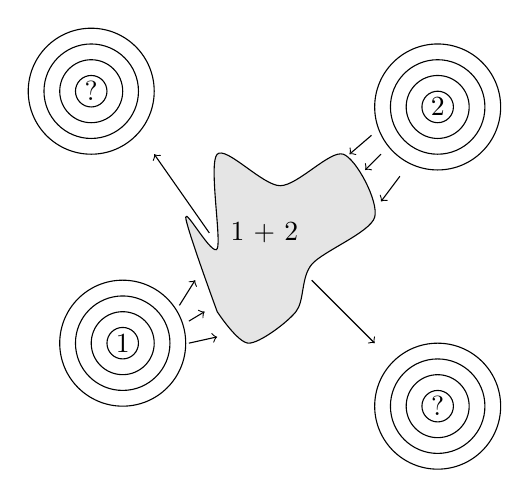
\begin{tikzpicture}[scale=0.4]
        \draw (0,0) circle (0.5);
        \draw (0,0) circle (1);
        \draw (0,0) circle (1.5);
        \draw (0,0) circle (2) node{1};
        \draw (10,7.5) circle (0.5);
        \draw (10,7.5) circle (1);
        \draw (10,7.5) circle (1.5);
        \draw (10,7.5) circle (2) node{2};
        \draw[fill=black!10] plot [smooth] coordinates{(3,1) (2,4) (3,3) (3,6) (5,5) (7,6) (8,4) (6,2.5) (5.5,1) (4,0) (3,1)};
        \draw (4.5,3.5) node{1 + 2};
        \draw[->] (1.8,1.2) -- (2.3,2);
        \draw[->] (2.1,0.7) -- (2.6,1);
        \draw[->] (2.1,0) -- (3,0.2);
        \draw[->] (8.2,6) -- (7.7,5.5);
        \draw[->] (7.9,6.6) -- (7.2,6);
        \draw[->] (8.8,5.3) -- (8.2,4.5);
        \draw[->] (6,2) -- (8,0);
        \draw[->] (2.75,3.5) -- (1,6);
        \draw (-1,8) circle (0.5);
        \draw (-1,8) circle (1);
        \draw (-1,8) circle (1.5);
        \draw (-1,8) circle (2) node{?};
        \draw (10,-2) circle (0.5);
        \draw (10,-2) circle (1);
        \draw (10,-2) circle (1.5);
        \draw (10,-2) circle (2) node{?};
    \end{tikzpicture}
    \hspace{3cm}
    \begin{tikzpicture}[scale=0.7]
        \draw plot [smooth] coordinates{(0,0) (2.5,2) (5,5)};
        \draw plot [smooth] coordinates{(2,-1) (4.5,2) (7,4)};
        \filldraw (0,0) circle (4pt) node[anchor=east]{1};
        \filldraw (7,4) circle (4pt) node[anchor=west]{2};
        \draw[<-] (5,5) -- (5.1,5,1);
        \draw[->] (2,-1) -- (1.9,-1.1);
    \end{tikzpicture}
\end{center}
\begin{multicols}{2}
    \textbf{qm:} Wellenpakete nach Stoß nicht merh den ursprünglichen Teilchen zuordenbar\\
    $\Rightarrow$ es ist sinnlos identische Teilchen zu nummerieren\\
    \textbf{klassisch:} man kann die Teilchen nummerieren und während des Stoßvorganges individuell verfolgen
\end{multicols}
\begin{center}
    $\Rightarrow$ weitreichende Konsequenzen
\end{center}

\subsubsection{Symmetrisierung}
\paragraph{Zwei-Teilchen-Zustände}
Teilchen-Vertauschungsoperator: $\widehat{P}_{12}$ (Austausch von Teilchen 1 und 2)

\begin{definition}{Teilchen-Vertauschungsoperator}
        \begin{align}
            \widehat{P}_{12} \ket{k_1,k_2} = \ket{k_2,k_1}
        \end{align}
\end{definition}
\begin{prop}{Eigenschaften des Teilchen-Vertauschungsoperators}
    \begin{align}
         &\rightarrow \widehat{P}_{12}\cdot \widehat{P}_{12} = \mathbb{1} \quad \Leftrightarrow \quad \widehat{P}_{12}^{-1} = \widehat{P}_{12}\\
            &\rightarrow \widehat{P}_{12} \text{ hermitesch, d.h. } \widehat{P}_{12}^{\dagger} = \widehat{P}_{12} \\
            &\rightarrow \text{Eigenwerte $\pi$ von }  \widehat{P}_{12} \ket{\varphi} = \pi \ket{\varphi} \ \text{ mit } \ (\widehat{P}_{12})^2 = \mathbb{1}\\
            &\qquad \Rightarrow \ket{\varphi} = \pi^2 \ket{\varphi} \ \Rightarrow \ \pi = \pm 1
    \end{align}
\end{prop}
\begin{proof}
    zur Hermitizität von $\widehat{P}_{12}$: Nutze Matrix in VON-Basis:
    \begin{align}
        \bra{k´,l´} \widehat{P}_{12} \ket{k,l} &= \bra{k´,l´}\ket{l,k} = \delta_{k´l}\delta_{l´k}  \label{eq:proof_hel_1}\\
        \bra{k´,l´} \widehat{P}_{12}^{\dagger} \ket{k,l} &= (\bra{k,l}\widehat{P}_{12}\ket{k´,l´})^* \\
        &= (\bra{k,l}\ket{l´,k}´)^* =\bra{l´,k´}\ket{k,l} = \delta_{l´k}\delta_{k´l} \label{eq:proof_hel_2}\\
        &\Longrightarrow (\ref{eq:proof_hel_1}) = (\ref{eq:proof_hel_2})
    \end{align}
\end{proof}

Sei $A$ eine Observable, die nicht zwischen Teilchenunterscheidet:
\begin{align}
    A \ket{k_1,k_2} &\stackrel{!}{=} \widehat{P}_{12}^{-1} \, A \, \widehat{P}_{12} \ket{k_1,k_2} \\
    &\Rightarrow A = \widehat{P}_{12}^{-1} \, A \, \widehat{P}_{12} \ \Rightarrow \ \widehat{P}_{12} A = A \widehat{P}_{12} \ \Rightarrow \ [A,\widehat{P}_{12}]=0
\end{align}
$H=\sum_i h_i$ macht keine Unterscheidung zwischen Teilchen (da $h \equiv h_i$)
\begin{itemize}
    \item[$\Rightarrow$] $[H,\widehat{P}_{12}]=0$
    \item[$\Rightarrow$] $\exists$ vollständiger Satz gemeinsamer Eigenzustände 
    \item[$\Rightarrow$] diese Eigenzustände sind in 2 Klassen einteilbar:
    \begin{align}
        \pi = +1 : \quad \ket{k_1,k_2}&+\ket{k_2,k_1} \quad \text{symmetrisch unter Vertauschung}\\
        \color{black!40} \widehat{P}_{12}\ket{k_1,k_2}&\color{black!40}+\widehat{P}_{12}\ket{k_2,k_1} = (+1)\cdot\ket{k_1,k_2} + (+1) \cdot \ket{k_2,k_1}\\
        \pi = -1 : \quad \ket{k_1,k_2}&-\ket{k_2,k_1} \quad \text{antisymmetrisch unter Vertauschung}\\
        \color{black!40} \widehat{P}_{12}\ket{k_1,k_2}&\color{black!40}-\widehat{P}_{12}\ket{k_2,k_1} = (-1)\cdot\ket{k_1,k_2} \underbrace{- (-1)}_{=+1} \cdot \ket{k_2,k_1}\\
        &\rightarrow \text{diese Zustände gibt es nur für } k_1 \neq k_2\\
        &\color{green!70!black} \rightarrow \text{Pauli-Prinzip} \color{black}
    \end{align}
\end{itemize}
Das Experiment zeigt, dass jeweils nur eine Klasse von Eigenzuständen auftritt!
\begin{beispiel}{Analogie zum unendlichen Kastenpotential}
\begin{multicols}{2}
    \begin{center}
    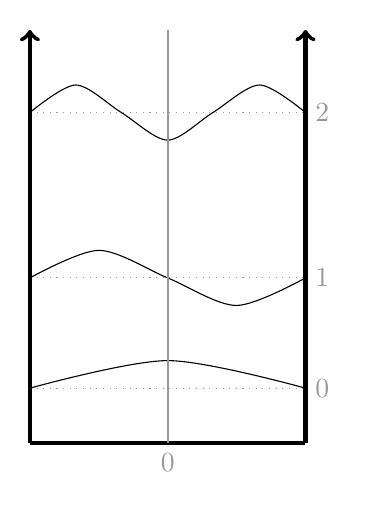
\begin{tikzpicture}[scale = 0.7]
        \draw[ultra thick,->] (0,0) -- (0,7.5);
        \draw[ultra thick,->] (5,0) -- (5,7.5);
        \draw[ultra thick] (0,0) -- (5,0);
        \draw[dotted,black!40] (0,1) -- (5,1) node[anchor=west]{0};
        \draw plot [smooth] coordinates{(0,1) (2.5,1.5) (5,1)};
        \draw[dotted,black!40] (0,3) -- (5,3) node[anchor=west]{1};
        \draw plot [smooth] coordinates{(0,3) (1.25,3.5) (2.5,3) (3.75,2.5) (5,3)};
        \draw[dotted,black!40] (0,6) -- (5,6) node[anchor=west]{2};
        \draw plot [smooth] coordinates{(0,6) (0.83,6.5) (1.66,6) (2.5,5.5) (3.32,6) (4.17,6.5) (5,6)};
        \draw[thick, black!40] (2.5,7.5) -- (2.5,0) node[anchor=north]{0};
    \end{tikzpicture}
    \end{center}
    \begin{itemize}
        \item[] Spiegelung um null
        \item[] 1.Klasse: nur symmetrisch
        \begin{itemize}
            \item[$\rightarrow$] Eigenzustände 0,2,4,...
        \end{itemize}
        \item[] 2. Klasse: nur antisymmetrisch
        \begin{itemize}
            \item[$\rightarrow$] Eigenzustände 1,3,5,...
        \end{itemize}
    \end{itemize}
\end{multicols}
\end{beispiel}

\begin{definition}{Symmetrisierungspostulat}
    Alle Zustände eines Systems aus identischen Teilchen sind unter Vertauschung entweder vollkommen symmetrisch und man nennt die Teilchen \emph{Bosonen} oder vollkommen antisymmetrisch und man nennt sie \emph{Fermionen}.
\end{definition}

\paragraph{Empirische Regel (Spin-Statistik-Theorem)}
\begin{itemize}
    \item Teilchen mit halbzahligem Spin ($\frac{1}{2},\frac{3}{2},..$) sind Fermionen
    \begin{itemize}
        \item Leptonen ($e,\mu,\tau,\nu_e,\nu_{\mu},\nu_{\tau}$) und Quarks ($u,d,s,c,b,t$)
    \end{itemize}
    \item Teilchen mit ganzzahligem Spin (0,1,2,...) sind Bosonen
    \begin{itemize}
        \item WW vermittelnden Teilchen:
        \begin{itemize}
            \item[] elm. WW: Photonen $\gamma$
            \item[] schwache WW: $W^{\pm}$, $Z^0$
            \item[] starke WW: Gluonen $g$
            \item[] Gravitation: Graviton 
        \end{itemize}
        \item kollektive Anregungen: Phononen, Plasmonen, Magnonen,...
        \item zusammengesetzte Teilchen:
        \begin{itemize}
            \item ungerade Anzahl Fermionen + beliebig viele Bosonen $\Rightarrow$ Fermion
            \begin{itemize}
                \item[] Baryonen (3 Quarks): Neutron, Proton
                \item[] $^3He$ (2 Protonen, 1 Neutron, 2 Elektronen) 
            \end{itemize}
            \item gerade Anzahl Fermionen + beliebig viele Bosonen $\Rightarrow$ Boson
            \begin{itemize}
                \item[] Mesonen (2 Quarks): Charmonium
                \item[] $^4He$ (2 Protonen, 2 Neutronen, 2 Elektronen) 
            \end{itemize}
        \end{itemize}
    \end{itemize}
\end{itemize}

\paragraph{Drei-Teilchen-Zustände}
\begin{itemize}
    \item[] Bosonen ($\pi=+1$, vollkommene Symmetrie)
    \begin{itemize}
        \item[*] $k_1 \neq k_2$, $k_1 \neq k_3$, $k_2 \neq k_3$
        \begin{equation}
            \ket{k_1,k_2,k_3} + \ket{k_2,k_3,k_1} + \ket{k_3,k_1,k_2} + \ket{k_2,k_1,k_3} + \ket{k_3,k_2,k_1} + \ket{k_1,k_3,k_2}
        \end{equation}
        \item[*] $k_1 = k_2 = k$, $k_3 \neq k$
        \begin{equation}
            \ket{k,k,k_3} + \ket{k_3,k,k} + \ket{k,k_3,k}
        \end{equation}
        \item[*] $k_1=k_2=k_3=k$
        \begin{equation}
            \ket{k,k,k}
        \end{equation}
    \end{itemize}
    \item[] Fermionen ($\pi = -1$, vollkommen antisymmetrisch)
    \begin{itemize}
        \item[*] $k_1 \neq k_2$, $k_1 \neq k_3$, $k_2 \neq k_3$
        \begin{align}
            \ket{k_1,k_2,k_3} + &\ket{k_2,k_3,k_1} + \ket{k_3,k_1,k_2} - \ket{k_2,k_1,k_3} - \ket{k_3,k_2,k_1} - \ket{k_1,k_3,k_2}\\
            &= det\begin{pmatrix}
                \ket{k_1} & \ket{k_1} & \ket{k_1}\\
                \ket{k_2} & \ket{k_2} & \ket{k_2}\\
                \ket{k_3} & \ket{k_3} & \ket{k_3}
            \end{pmatrix}
        \end{align}
        \item[*] keine weiteren Zustände
    \end{itemize}
\end{itemize}
\subparagraph{Bemerkung}
Es gibt mehr Mikrozustände für Bosonen als für Fermionen!

\paragraph{Vielteilchenzustände}
\begin{itemize}
    \item Bosonen ($\pi = +1$, vollkommen symmetrisch):\\
    alle $k_i$ unterschiedlich ($k_n\neq k_m$ $\forall n\neq m$)
    \begin{align}
        \frac{1}{\sqrt{N!}} \sum_{\gamma =1}^{N!} P_{\gamma} \ket{k_1,k_2,...,k_N} \quad P_{\gamma}\text{ erzeuge alle N' Permutationen}
    \end{align}
    einige der $k_i$ haben gleiche Werte $k_j$ kommt $n_j$ mal vor, $j=1,...,J<N$
    \begin{align}
        \frac{1}{\sqrt{S}} \sum_{\gamma = 1}^S P'_{\gamma} \ket{k_1,k_2,...,k_N} \quad P'_{\gamma} \text{ erzeuge alle Permutationen der Dopplung}\\
        S=\frac{N!}{n_1!n_2!...n_J!}
    \end{align}
    \item Fermionen ($\pi = -1$, vollkommen antisymmetrisch):
    \begin{align}
        \frac{1}{\sqrt{N!}} \sum_{\gamma =1}^{N!} (-1)^{\tau} P_{\gamma} \ket{k_1,k_2,...,k_N} 
        =\frac{1}{\sqrt{N}} \underbrace{\det \mqty(\ket{k_1} & \ket{k_1} & ... & \ket{k_1} \\ \ket{k_2} & \ket{k_2} & ... & \ket{k_2} \\ ... & ... & &... \\ \ket{k_N} & \ket{k_N} & ... & \ket{k_N})}_{\text{Slater-Determinante}}
    \end{align}
    hier darf kein $k_i=k_j$ sein, sonst zwei gleiche Zeilen in Determinante $\Rightarrow$ Zustand verschwindet: Pauli-Prinzip
\end{itemize}
\subparagraph{Anmerkung}
Diese Schreibweise der Symmetrisierung wird hier nicht gebraucht



\subsubsection{Fockraum, Besetzungszahldarstellung} \marginpar{VL 19}

\paragraph{Ziel:} Schreibweise ohne umständliche Symmtrisierung
\begin{definition}{Fockraum}
    Betrachte Einteilchenzustände $\ket{0},\ket{1},...$ und gebe an, mit wie vielen Teilchen besetzt\\
    $\Rightarrow$ Besetzungszahl $n_k$ des Einteilchenzustands $\ket{k}$\\
    $\Rightarrow$ $\ket{n_0,n_1,n_2,...,n_k,...}$ ist Zustand in Fockraum ($\ket{n_0}=$ Teilchen im Einteilchenzustand $\ket{0}$)
\end{definition}


\begin{beispiel}{Beispiele}
    \begin{itemize}
        \item $\ket{n_0,n_1,n_2,...,n_k,...}$ ist Zustand im Fockraum
        \begin{itemize}
            \item[] mit $n_0$ im Einteilchen-Grundstustand $\ket{0}$,
            \item[] ...,
            \item[] mit $n_k$ im Einteilchen-Zustand $\ket{k}$,
            \item[] ...
        \end{itemize}
        \item Vakuum: $\ket{0,0,0,...}$
        \item Einteilchenzustand $\ket{k}$: $\ket{0,0,...,0,1,0,...}$
    \end{itemize}
\end{beispiel}
\paragraph{Bemerkung:}
\begin{itemize}
    \item Zahl der Teilchen nicht festgelegt
    \item Bosonen: $n_k = 0,1,2,...$
    \item Fermionen: $n_k = 0,1$
    \item Symmetrisierung (damit) berücksichtigt
\end{itemize}



\begin{definition}{Besetzungszahloperator $\hat{n}_k$}
    \begin{align}
        \hat{n}_k \ket{n_0,n_1,...,n_k}= n_k \ket{n_0,n_1,...,n_k,...}
    \end{align}
\end{definition}
\color{black!40}
Später:
    \begin{align}
        \hat{n}_k = a_k^+a_k
    \end{align}
    Man nennt dies auch die 2. Quantisierung (erst Einteilchezustände $\ket{k}$ und jetzt $n_k$ als Quantenzahlen). Die $a_k$ sind dabei für Fermionen und Bosonen unterschiedlich (siehe Quantentheorie 2).
\color{black}

\begin{definition}{Teilchenzahloperator}
    \begin{align}
        \hat{N} = \sum_{k=0}^{\infty} \hat{n}_k
    \end{align}
\end{definition}

\begin{definition}{Hamiltionoperator mit Besetzungszahloperator}
    \begin{align}
        \hat{H} = \sum_k \hat{n}_k \varepsilon_k
    \end{align}
\end{definition}


\begin{beispiel}{2 Niveau System}
    Einteilchenzustände $\ket{a},\ket{b}$
    \begin{multicols}{2}
       \begin{itemize}
        \item 1 Teilchen ($\ket{a},\ket{b}$:\\
        Einteilchen-Darst.: $\ket{a},\ket{b}$\\
        Besezungszahl.: $\ket{1,0},\ket{0,1}$
        \item Teilchen, Bosonen\\
        Zweiteilchen-Darst.: $\ket{a,a} \frac{1}{\sqrt{2}}(\ket{a,b}-\ket{b,a}) \ket{b,b}$\\
        Besetzungsgrad.: $\ket{2,0} \ket{1,1} \ket{0,2}$\\
        $\Rightarrow$ 3 Zustände
        \item 2 Teilchen, Fermionen\\
        Zweiteilchen-Darst.: $\frac{1}{\sqrt{2}}(\ket{a,b}-\ket{b,a})$\\
        Besetzungszahl.: $\ket{1,1}\\
        \Rightarrow$ 1 Zustand
        \item 2 Teilchen, klassische unterscheidbar\\
        Klass. Berücksichtigung der Ununterscheidbarkeit: Faktor $\frac{1}{N!}$\\
        $\Rightarrow$ 2 Zustände
        $\Rightarrow$ M-B-Stat.
        \end{itemize} 
        \begin{center}
            \begin{tikzpicture}[scale = 0.5]
                \draw[thick,red] (3,0) -- (0,0) node[anchor=east]{$\varepsilon_a$};
                \draw[thick,red] (3,1) -- (0,1) node[anchor=east]{$\varepsilon_b$};
                \filldraw[black] (1,0) circle (3pt);
                \filldraw[green] (2,0) circle (3pt);
                \draw[thick,red] (4,0) -- (7,0);
                \draw[thick,red] (4,1) -- (7,1);
                \filldraw[black] (5,0) circle (3pt);
                \filldraw[green] (6,1) circle (3pt);
                \draw[thick,red] (8,0) -- (11,0);
                \draw[thick,red] (8,1) -- (11,1);
                \filldraw[black] (9,1) circle (3pt);
                \filldraw[green] (10,0) circle (3pt);
                \draw[thick,red] (12,0) -- (15,0);
                \draw[thick,red] (12,1) -- (15,1);
                \filldraw[black] (13,1) circle (3pt);
                \filldraw[green] (14,1) circle (3pt);
                
                \draw[thick,red] (3,4) -- (0,4) node[anchor=east]{$\varepsilon_a$};
                \draw[thick,red] (3,5) -- (0,5) node[anchor=east]{$\varepsilon_b$};
                \filldraw[black] (1.5,4) circle (3pt);
                \filldraw[black] (1.5,5) circle (3pt);
                
                \draw[thick,red] (3,8) -- (0,8) node[anchor=east]{$\varepsilon_a$};
                \draw[thick,red] (3,9) -- (0,9) node[anchor=east]{$\varepsilon_b$};
                \filldraw[black] (1,8) circle (3pt);
                \filldraw[black] (2,8) circle (3pt);
                \draw[thick,red] (4,8) -- (7,8);
                \draw[thick,red] (4,9) -- (7,9);
                \filldraw[black] (5,8) circle (3pt);
                \filldraw[black] (6,9) circle (3pt);
                \draw[thick,red] (8,8) -- (11,8);
                \draw[thick,red] (8,9) -- (11,9);
                \filldraw[black] (9,9) circle (3pt);
                \filldraw[black] (10,9) circle (3pt);

                \draw[thick,red] (3,12) -- (0,12) node[anchor=east]{$\varepsilon_a$};
                \draw[thick,red] (3,13) -- (0,13) node[anchor=east]{$\varepsilon_b$};
                \filldraw[black] (1.5,12) circle (3pt);
                \draw[thick,red] (4,12) -- (7,12);
                \draw[thick,red] (4,13) -- (7,13);
                \filldraw[black] (5.5,13) circle (3pt);
            \end{tikzpicture}
        \end{center}
    \end{multicols}
     
\end{beispiel}
\begin{itemize}
    \item[$\rightarrow$] Besetzungszahldarstellung für klassische Teilchen nicht möglich
    \item[$\rightarrow$] klassische Berücksichtigung der Ununterscheidbarkeit durch Faktor $\frac{1}{N!}$ (Maxwell-Boltzmann-Statistik $\Rightarrow$ effektiv 2 Zustände (liegt zwischen Fermionen und Bosonen))
\end{itemize}


\subsubsection{Zustandssumme}
kanonische Zustandssumme für $N$ Teilchen: $Z=\trace\left(e^{-\beta H}\right)$
\begin{align}
    Z =\trace\left(e^{-\beta H}\right)&= \sum_{n_0,n_1,...}\ev{e^{-\beta \sum_k \varepsilon_k \hat{n}_k}}{n_0,n_1,...} \quad \text{mit} \sum_k n_k=N\\
    &= \sum_{n_0,n_1,...} e^{-\beta \sum_k \varepsilon_k n_k} = \sum_{n_0,n_1,...} \prod_k e^{-\beta \varepsilon_k n_k}\\
    &\rightarrow \text{weitere Umformungen wegen Summeneinschränkung schwierig}
\end{align}

\begin{beispiel}{2 Einteilchenzustände}
    N=3 $\Rightarrow$ $\ket{3,0}, \ \ket{2,1}, \ \ket{1,2},\ \ket{0,3}$
\end{beispiel}

großkanonische Zustandssumme:
\begin{itemize}
    \item Vorteil: N beliebig $\Rightarrow$ keine Einschränkung an Summe
    \item Nachteil: chem. Potential $\mu$ statt N
\end{itemize}
\begin{align}
    Z_G =  \trace\left( e^{-\beta (\hat{H}-\mu) \hat{N}}\right)&= \underbrace{\sum_{n_0,n_1,...}}_{\text{bel. Besetz. ET-Zustände}} \ev{e^{-\beta ( \sum_k (\varepsilon_k-\mu) \hat{n}_k)}}{n_0,n_1,...}\\
    &= \sum_{n_0,n_1,...} e^{-\beta \sum_k(\varepsilon_k-\mu)n_k}=\sum_{n_0,n_1,...} \prod_k \underbrace{e^{-\beta(\varepsilon_k-\mu)n_k}}_{(X_n)^{n_k}} \\
    &\overset{*}{=} \prod_k \sum_{n_k} (X_n)^{n_k}
\end{align}
zu ($*$)
\begin{align}
    (X_0)^0\cdot(X_1)^0 &+ (X_0)^1\cdot(X_1)^0 + (X_0)^0\cdot(X_1)^1 + (X_0)^2\cdot(X_1)^0 + (X_0)^1\cdot(X_1)^1 + (X_0)^0\cdot(X_1)^2 + ... \\
    &= \left[ (X_0)^0 + (X_0)^1 + (X_0)^2 + ... \right] \left[ (X_1)^0 + (X_1)^1 + (X_1)^2 + ... \right]
\end{align}
$\rightarrow$ Vertauschung von $\Sigma$ und $\Pi$ nur möglich, da N beliebig\\
(richtig: Reihe konvergent, da Zustände und e-Fkt. > 0 $\Rightarrow$ absolut konvergent $\Rightarrow$ Cauchy-Produkt)\\
\textbf{Fermionen:}
\begin{align}
    \sum_{n_k=0,1} (X_k)^{n_k} = 1 + X_k
\end{align}
\begin{definition}{Zustandssumme Fermionen}
    \begin{align}
        Z_G = \prod_k (1+ e^{-\beta(\varepsilon_k - \mu)})
    \end{align}
\end{definition}
\textbf{Bosonen:}
\begin{align}
    \sum_{n_k=0}^\infty (X_k)^{n_k} = \frac{1}{1-X_k}
\end{align}
\begin{definition}{Zustandssumme Bosonen}
    \begin{align}
        Z_G = \prod_k \frac{1}{1-e^{-\beta(\varepsilon_k-\mu)}}
    \end{align}
    gilt nur falls: $ \abs{X_k}<1 \Leftrightarrow \beta(\varepsilon_k-\mu) > 0 \Leftrightarrow \mu < \varepsilon_k \forall k$ insbesondere $\mu < \varepsilon_0$ Grundzustandsenergie. Dies ist eine phy. sinnvolle Einschränkung, da sonst $\infty$ Bosonen im Grundzustand (kein GG möglich, da alle Teilchen aus Reservoir in Grundzustand gehen würden)
\end{definition}

\subsubsection{Großkanonisches Potential und mittlere Besetzungszahl} \marginpar{VL 20}

\begin{definition}{Großkanonisches Potential}
    \begin{equation}
        \Phi(\beta,V,\mu) = - \frac{1}{\beta} \ln(Z_G) = \mp \frac{1}{\beta} \sum_k \ln\left(1 \pm e^{-\beta(\varepsilon_k-\mu)}\right)
    \end{equation}
\end{definition}
\begin{center}
    (oberes VZ Fermionen, unteres VZ Bosonen ($\mu < \varepsilon_0$))
\end{center}
Bemerkung: $\beta$, $\mu$ explizit, V beeinflusst Einteilchenenergien $\varepsilon_k$
\begin{center}
    $\Longrightarrow$ alle thermodynamischen Eigenschaften berechenbar
\end{center}
\begin{align}
    \Phi(T,V,\mu) &= U - TS -\mu N\\
    d\Phi &= - S \ dT - p \ dV - N \ d\mu
\end{align}

\paragraph{mittlere Teilchenzahl}
\begin{equation}
    \expval{\hat{N}}(\beta,V,\mu) = - \left(\pdv{\Phi}{\mu}\right)_{T,V} = \pm \frac{1}{\beta} \sum_k \frac{\pm e^{-\beta(\varepsilon_k-\mu)}\cdot \beta}{1 \pm e^{-\beta(\varepsilon_k-\mu)}} = \sum_k \frac{1}{e^{\beta(\varepsilon_k-\mu)}\pm 1}
\end{equation}
$\rightarrow$ Zusammenhang mittlere Teilchenzahl und chemisches Potential

\paragraph{mittlere Besetzungszahl von Einteilchenzustand $k$}
\begin{align}
    \qq*{vergleiche:} \expval{\hat{N}} &= \sum_k \expval{\hat{n}_k} \qq{(Annahme)} \\
    \Longrightarrow \quad \expval{\hat{n}_k} &=
    \begin{cases}
        \frac{1}{e^{\beta(\varepsilon_k-\mu)}+1} \qquad \text{Fermionen: Fermi-Dirac-Statistik} \\
        \frac{1}{e^{\beta(\varepsilon_k-\mu)}-1} \qquad \text{Bosonen: Bose-Einstein-Statistik } (\mu< \varepsilon_0)
    \end{cases}
\end{align}

Jetzt explizite Rechnung:
\begin{align}
    \expval{\hat{n}_k} = \trace(\hat{\varrho}\hat{n}_k) &= \sum_{n_0,n_1,...} n_k \, p(\ket{n_0,n_1,..})\\ \color{black!50}
    \hat{\varrho} &= \color{black!50}\frac{e^{-\beta(\hat{H}-\mu\hat{N})}}{Z_G} \\
    \color{black!50}p(\ket{n_0,n_1,...}) &= \color{black!50}\frac{1}{Z_G} e^{-\beta \sum_k (\varepsilon_k-\mu)n_k}\\
    &= \frac{1}{Z_G} \sum_{n_0,n_1,..} n_k \, e^{-\beta \sum_k (\varepsilon_k-\mu)n_k}\\
    &= \frac{1}{Z_G} \left(-\frac{1}{\beta} \right) \pdv{\varepsilon_k} \underbrace{\sum_{n_0,n_1,...} e^{-\beta \sum_k (\varepsilon_k-\mu)n_k}}_{Z_G} = -\frac{1}{\beta} \pdv{\varepsilon_k} \ln(Z_G)\\
    &= -\frac{1}{\beta} \pdv{\varepsilon_k} \ln\left(\left(1 \pm e^{-\beta(\varepsilon_k-\mu)}\right)^{\pm 1} \right) = - \frac{1}{\beta} \frac{e^{-\beta(\varepsilon_k-\mu)} \cdot (-\beta)}{1 \pm e^{-\beta(\varepsilon_k-\mu)}} \\
    &= \frac{1}{e^{+\beta(\varepsilon_k-\mu)}\pm 1} \qquad \checkmark
\end{align}
\begin{center}
    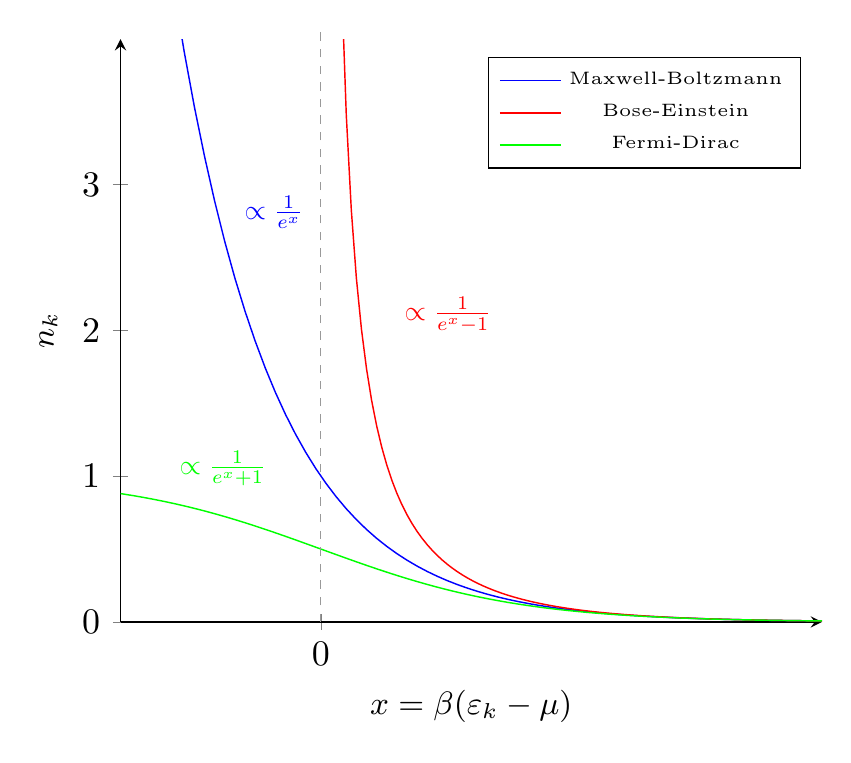
\begin{tikzpicture}[scale=1.3]
        \begin{axis}[
        axis lines = left,
        xlabel ={\small $x=\beta (\varepsilon_k-\mu)$},
        ylabel = {\small $\expval{n_k}$},
        xmin= -2, xmax=5,
        ymin=0, ymax=4,
        xtick = {0}, xticklabels = {0},
        ytick={0,1,2,3}, yticklabels= {0,1,2,3},
        legend pos=north east,
        ]
        \addplot[samples=100, color=blue]{1/(e^x)};
        \addplot[domain=0:5, samples=100, color=red]{1/(e^x-1)};
        \addplot[samples=100, color=green]{1/(e^x+1)};
        \legend{\tiny Maxwell-Boltzmann, \tiny Bose-Einstein, \tiny Fermi-Dirac}
        \end{axis}
        \draw[red] (3.2,3) node{$\propto \frac{1}{e^x-1}$};
        \draw[blue] (1.5,4) node{$\propto \frac{1}{e^x}$};
        \draw[green] (1,1.5) node{$\propto \frac{1}{e^x+1}$};
        \draw[dashed, black!40] (1.95,0) -- (1.95,5.8);
    \end{tikzpicture}
\end{center}
\begin{itemize}
    \item[] Besetzungszahl $n_k \ll 1$ (geringe Teilchendichte)
    \begin{itemize}
        \item[$\Rightarrow$] Statistik gleich 
    \end{itemize}
    \item[] Besetzungszahl $n_k \gg 1$ (Bosonen, hohe Teilchendichte) oder $n_k \approx 1$ (Fermionen)
    \begin{itemize}
        \item[$\Rightarrow$] neue Quantenphänomene für Fermionen / Bosonen 
    \end{itemize}
\end{itemize}

\begin{center}
    \begin{tikzpicture}
        \draw[ultra thick, <-] (0,7) -- (0,0) node[anchor=north]{Fermionen};
        \draw[ultra thick, <-] (7,7) -- (7,0) node[anchor=north]{Bosonen};
        \draw[ultra thick] (6.9,5.5) -- (7.1,5.5) node[anchor=west]{$\varepsilon_0$};
        \draw[ultra thick] (0.1,1) -- (-0.1,1) node[anchor=east]{$\varepsilon_0$};
        \draw[ultra thick] (0.1,2) -- (-0.1,2) node[anchor=east]{$\varepsilon_1$};
        \draw[ultra thick] (0.1,3) -- (-0.1,3) node[anchor=east]{$\varepsilon_2$};
        \draw[ultra thick] (0.1,4) -- (-0.1,4) node[anchor=east]{$\varepsilon_3$};
        \draw[ultra thick] (0.1,5) -- (-0.1,5) node[anchor=east]{$\varepsilon_4$};
        \draw[ultra thick] (0.1,6) -- (-0.1,6) node[anchor=east]{$\varepsilon_5$};
        \draw[thick, black!40] (1,4.5) -- (6,4.5) node[anchor=north west]{$\mu$};
        \fill[black!40, pattern=north east lines] (1,0) rectangle (6,4.5);
        \draw[thick] (0.5,4.5) -- (0.5,1);
        \draw[thick] (0.4,4.5) -- (0.6,4.5);
        \draw[thick] (0.4,1) -- (0.6,1);
        \draw[thick] (6.5,4.5) -- (6.5,5.5);
        \draw[thick] (6.4,4.5) -- (6.6,4.5);
        \draw[thick] (6.4,5.5) -- (6.6,5.5);
        \draw[black!60] (0,-1) node{(je ein Teilchen in Zuständen};
        \draw[black!60] (0,-1.5) node{mit $\varepsilon_k < \mu$)};
        \draw[black!60] (7,-1) node{(Divergenz $\widehat{=}$};
        \draw[black!60] (7,-1.5) node{immer mehr Teilchen würden};
        \draw[black!60] (7,-2) node{in Grundzustand gelangen)};
        
    \end{tikzpicture}
\end{center}

\subparagraph{Bemerkung:}
\begin{itemize}
    \item physikalische Bedeutung von $x \gg 1 \, \Leftrightarrow \ \varepsilon_0-\mu \gg kT$ (bei wenigen Teilchen ist Unterschied zwischen Fermionen und Bosonen gering)
    \begin{itemize}
        \item[$\rightarrow$] nicht zu interpretieren als $T \to 0$, sondern als $n_k \to 0$, d.h. klassischer Grenzfall 
    \end{itemize}
    \item weitere Größen:
    \begin{equation}
        p = \left(\pdv{\Phi}{V}\right)_{T,\mu} \qquad S = - \left( \pdv{\Phi}{T}\right)_{V,\mu}
    \end{equation}
    \item thermische Zustandsgleichung und Adiabatengleichung $\rightarrow$ Übung 12.2
\end{itemize}

\subsubsection{Klassischer Grenzfall}
\begin{itemize}
    \item mittlere Besetzungszahl klein: $\expval{n_k} \ll 1 \, \Leftrightarrow \, e^{\beta(\varepsilon_k-\mu)}\gg 1$
    \begin{equation}
        \Rightarrow \ \expval{n_k} \approx \frac{1}{e^{\beta(\varepsilon_k-\mu)}} = e^{-\beta(\varepsilon_k-\mu)} \qq{Maxwell-Boltzmann Statistik}
    \end{equation}
    \item Näherung in Zustandssumme berücksichtigen:
    \begin{align}
        \ln(Z_G) &= \pm \sum_k \underbrace{\ln\left(1 \pm e^{-\beta(\varepsilon_k-\mu)}\right)}_{\stackrel{Taylor}{\approx} \pm e^{-\beta(\varepsilon_k-\mu)}} \approx e^{\beta \mu} \underbrace{\sum_k e^{-\beta \varepsilon_k}}_{=: Z(\beta,V)}\\
        Z_G &\approx e^{Z \cdot e^{\beta\mu}} \stackrel{Taylor}{\approx} \sum_{N=0}^{\infty} \frac{1}{N!} Z(\beta,V)^N e^{\beta\mu N}
    \end{align}
    \item vergleiche mit:
    \begin{align}
        Z_G(\beta,V,N) &= \trace\left(e^{-\beta(\hat{H}-\mu \hat{N})}\right) = \sum_{N=0}^{\infty} \sum_{\substack{n_0,n_1,...\\\sum_k n_k = N}} e^{-\beta \sum_k (\varepsilon_k-\mu)n_k} \\
        &= \sum_{N=0}^{\infty} e^{\beta\mu N} \underbrace{\sum_{\substack{n_0,n_1,...\\\sum_k n_k = N}} e^{-\beta \sum_k \varepsilon_k n_k}}_{\substack{Z(\beta,V,N) \\ \text{kan. ZS f. N Teilchen}}} = \sum_{N=0}^{\infty} Z(\beta,V,N) e^{\beta \mu N}
    \end{align}
    \begin{definition}{Maxwell-Boltzmann-Näherung}
        \begin{equation}
            Z(\beta,V,N) \approx \frac{1}{N!} Z(\beta,V)^N
        \end{equation}
    \end{definition}
    \begin{itemize}
        \item[] klassische Beschreibung ideales Gas aus Quantenmechanik hergeleitet
        \begin{itemize}
            \item zunächst unterscheidbare Teilchen (aber indentisch): $Z^N$
            \item Berücksichtigung der Ununterscheidbarkeit durch Faktor $\frac{1}{N!} \quad \widehat{=} \quad$ Gibbs 
        \end{itemize}
    \end{itemize}
\end{itemize}

\subsubsection{Kontinuumslimes} \marginpar{VL 21}\label{abs.Kontinuumslimes}

\begin{itemize}
    \item bisher $\sum_{k=0}^\infty f(\varepsilon)$ d.h. Summe über Einteilchenzustände mit Energie $\varepsilon_k$.
    \item  Volumen $V \rightarrow \infty \hspace{2cm} \Rightarrow$ Zustandsdichte wird immer feiner (d.h. Kontinuierlich) 
    genaue Werte $\varepsilon_k$ nicht relevant sondern mittleres Verhalten
    \end{itemize}

    \paragraph{Impulsintegration in 3D}
    \begin{align}
         \sum_{k=0}^\infty ... \longrightarrow &\underbrace{2s+1}_{\text{Zahl der Spinzustände}} \underbrace{\frac{1}{h^3}}_{\text{Planck in 3D}} \underbrace{\int d^3q}_{V} \underbrace{\int d^3p}_{4\pi \int_0^\infty dp \, p^2} \\
   &(2s+1) \ \frac{V}{h^3}\  4\pi \ \int dp \, p^2
    \end{align}

\paragraph{k-Raum Integration in 3D $\Vec{p} =\hbar \Vec{k}$}

\begin{equation}
    \sum_{k=0}^\infty... \longrightarrow (2s+1) \left( \frac{L}{2\pi}\right)^3 \int_0^\infty dk \, k^2
\end{equation}

alternativ am Bsp. Teilchen im Kastenpotential mit Breite L
\begin{equation}
    \Psi_n (x)= \sinh \left( n \frac{\pi x}{L} \right)  \approx e^{ikx} - e^{-ikx}
\end{equation}

mit Wellenvektor $k=n \frac{\pi}{L}$

\begin{equation}
    \sum_{K=1}^\infty ... \longrightarrow \int_0^\infty dn \overset{k=n\frac{\pi}{L}}{=} \frac{L}{\pi } \int_0^\infty dk = \frac{L}{2\pi} \int_{-\infty}^\infty dk
\end{equation}

\paragraph{Energie-Integration}
Zustandsdichte:
\begin{align}
    d(\varepsilon) &= \sum_{k=0}^\infty \delta (\varepsilon-\varepsilon_k)\\
    \sum_{k=0}^\infty  f(\varepsilon_k) &\overset{\text{exakt}}{=} \int d\varepsilon \ d((\varepsilon)) \ f(\varepsilon) \\
    &= \int d\varepsilon \underbrace{\Bar{d}(\varepsilon)}_{\text{geglättete Zustandsdichte}} f(\varepsilon)
\end{align}
\begin{center}
    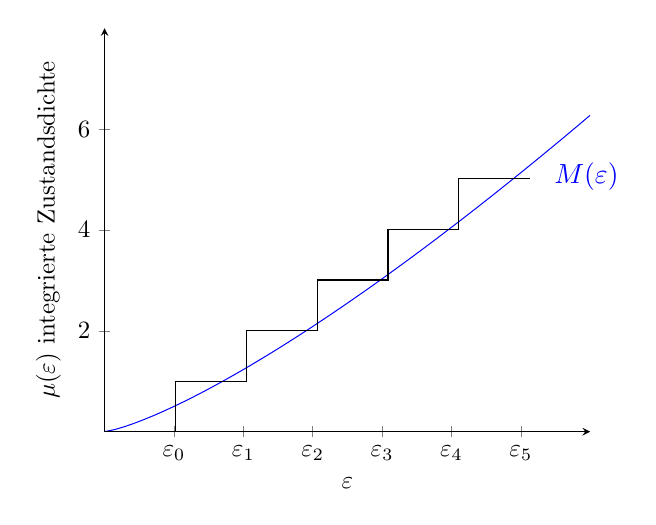
\begin{tikzpicture}[scale=0.9]
        \begin{axis}[
        axis lines = left,
        xmin=0, xmax=7,
        ymin=0, ymax=8,
        xlabel={$\varepsilon$},
        ylabel={$\mu(\varepsilon)$ integrierte Zustandsdichte},
        xtick={1,2,3,4,5,6},
        ytick={2,4,6},
        xticklabels={$\varepsilon_0$,$\varepsilon_1$,$\varepsilon_2$, $\varepsilon_3$,$\varepsilon_4$,$\varepsilon_5$}
        ]
        \addplot[color=blue,samples=50,domain=0:7]{0.5*x^(1.3)};
        \end{axis}
        \draw (0,0) -- (1,0) -- (1,0.713) -- (2,0.713) -- (2,1.426) -- (3,1.426) -- (3,2.14) -- (4,2.14) -- (4,2.853) -- (5,2.853) -- (5,3.566) -- (6,3.566);
        \draw[blue] (6.8,3.6) node{$\Bar{M}(\varepsilon)$};
    \end{tikzpicture}
\end{center}

Im folgenden Querstrich $\Bar{d}$ wird weggelassen

\begin{beispiel}{Bsp}
    \begin{align}
        N &= \int d\varepsilon \ d(\varepsilon) n_\varepsilon \\
        n_\varepsilon &= \frac{1}{e^{\beta (\varepsilon-\mu)}} \pm 1\\
        U &= \int d\varepsilon \ d(\varepsilon) \ \varepsilon \ n_\varepsilon 
    \end{align}
    
     Nutze Energie-Impuls-Relation $\varepsilon(p)$:

     \begin{itemize}
         \item \textbf{Freies Teilchen} 
         \begin{equation}
             \varepsilon (p) = \sqrt{m^2c^4+ c^2p^2} = \begin{cases}
                 mc^2+\frac{p^2}{2m} \ , \frac{p}{m} \ll c \text{  nicht relativistisch}\\
                 cp \ , \text{ mit } m=0 \text{ hochrelativistischer Grenzfall (Photonen)}
             \end{cases}
         \end{equation}
         \item  andere $\varepsilon(p) , z.b. Phononen$
     \end{itemize}
\end{beispiel}

\begin{beispiel}{1 Teilchen in 3D-Volumen mit Spin $s$ und Dispersion $\varepsilon(p) = \frac{p^2}{2m}$}
    Zustandsdichte
    \begin{align}
        d(\varepsilon) & = \sum_k \delta(\varepsilon-\varepsilon_k) = (2s+1) \frac{V}{h^3} \ 4\pi \int_0^\infty dp \ p^2 \ \underbrace{\delta(\varepsilon-\varepsilon_l) }_{\delta(p-\sqrt{2m\varepsilon}) \frac{m}{p}}\\
      \Rightarrow \ d(\varepsilon)  &= (2s+1) 4\pi \sqrt{2} \ \frac{V m^{3/2}}{h^3} \sqrt{\varepsilon} \ \Theta(\varepsilon)
    \end{align}
        
  \textbf{Bem.:} abhängig von Dimension und Dispersion $\varepsilon(p)$. Sei $\varepsilon(p) = \frac{p^2}{2m}$ 
    \begin{align}
        d=3 && d(\varepsilon) \sim \varepsilon^{1/2}\\
        d=2 && d(\varepsilon) \sim \varepsilon^{0}\\
        d=1 && d(\varepsilon) \sim \varepsilon^{-1/2}
    \end{align}
\end{beispiel}


\paragraph{Mittlere Teilchenzahl in 3D -Volumen:}
\begin{align}
    N &= \int d\varepsilon \ d(\varepsilon) \ n_\varepsilon = (2s+1)4\pi \sqrt{2} \frac{V m^{3/2}}{h^3} \int_0^\infty d\varepsilon \sqrt{\varepsilon} \underbrace{\frac{1}{e^{\beta (\varepsilon-\mu)} \pm 1}}_{n_\varepsilon} \\
    &\overset{x=p\varepsilon}{=} \frac{V}{\lambda^3} (2s+1)\frac{2}{\sqrt{\pi}} \int dx \frac{x^{1/2}}{e^{x-\beta\mu} \pm 1}\\
    \lambda &:= \frac{h}{\sqrt{2\pi mkT}} \ \text{thermische De-Broglie Wellenlänge}
\end{align}

Klassischer Grenzfall:
 \begin{align}
     n_\varepsilon \ll 1 && \Leftrightarrow && e^{\beta(\varepsilon-\mu) } \gg 1
 \end{align}
\begin{equation}
    N \approx \frac{V}{\lambda^3} \ (2s+1)  \ \underbrace{\frac{2}{\sqrt{\pi}}\  \int_0^\infty dx \ \frac{x^{1/2}}{e^{x-\beta\mu}}}_{\Gamma(1/2 =1}
\end{equation}

\begin{equation}
    \frac{N\lambda^3}{V \, (2s+1)} = e^{\beta \mu} \overset{\varepsilon \approx 0}{\ll} 1
\end{equation}

\begin{equation}
    \Longrightarrow \quad \fcolorbox{green!70!black}{white}{$\lambda \ll \left(\frac{V}{N}\right)^{1/3}$} \qq{klassicher Grenzfall}
\end{equation}

thermische Wellenlänge $\ll$ typischer Abstand  (erfüllt für: kleine Dichte $\frac{N}{V} \rightarrow 0$ , hohe Temperatur $\lambda \rightarrow 0$)

\textbf{Bem.:} Man kann zeigen (nächste Ordnung in Störungstheorie)
\begin{equation}
    \frac{pV}{mkT} = 1 \pm \frac{\lambda^3}{(2s+1) 2^{3/2}} \frac{N}{V} \begin{cases}
        \text{Fermionen}\\ \text{Bosonen}
    \end{cases}
\end{equation}

\begin{itemize}
    \item Fermionen:  höherer Druck $\rightarrow$ effektive Abstoßung
    \item Bosonen:  niedriger Druck $\rightarrow$ effektive Anziehung
\end{itemize}

\subsection{Fermi-Gas}

\begin{align}
    \hat{H} &= \sum_k \varepsilon_k \hat{n}_k \\
    \langle \hat{n}_k \rangle &= \frac{1}{e^{\beta (\varepsilon_k -\mu)} +1} = f(\varepsilon)  \ \text{Fermi-Fkt.}\\
    \hat{N} &= \sum_k\hat{n}_k
\end{align}
\begin{center}
    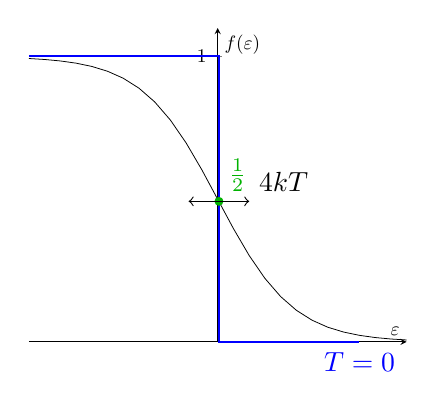
\begin{tikzpicture}[scale=.7]
        \begin{axis}[
        axis lines = center,
        xtick=\empty,
        ytick={0,1},
        ymin=0, ymax=1.1,
        xlabel=$\varepsilon$,
        ylabel=$f(\varepsilon)$
        ]
        \addplot[black]{1/(e^(x)+1)};            
        \end{axis}
        \draw[thick, blue](0,5.18) -- (3.45,5.18) -- (3.45,0) -- (6,0) node[anchor=north]{$T=0$};
        \filldraw[green!70!black] (3.45,2.55) circle (2pt) node[anchor=south west]{$\frac{1}{2}$};
        \draw[<->] (2.9,2.55) -- (4,2.55) node[anchor=south west]{$4kT$};
    \end{tikzpicture}
\end{center}
Ableitung bei $\varepsilon-\mu$:
\begin{equation}
    \abl{f(\varepsilon)}{\varepsilon}\bigg|_{\varepsilon=\mu} =  - \frac{e^{\beta (\varepsilon-\mu)} \beta}{\left( e^{\beta (\varepsilon-\mu)} +1 \right)^2} \bigg|_{\varepsilon=\mu} = -\frac{\beta}{4} =-\frac{1}{4kt}
\end{equation}

Symmetrie:
\begin{align}
    f(\varepsilon) &= \frac{1}{2} - \frac{1}{L} \tanh \left( \frac{\varepsilon-\mu}{2kT} \right) \\
    f(\varepsilon) &\overset{T\to 0}{\longrightarrow }\Theta(\varepsilon-\mu)
\end{align}
\begin{multicols}
    {} Fermi-Energie $\varepsilon_F$ ist definiert für $T=0$. $\varepsilon_F$ zwischen höchster besetzter und niedrigster unbesetzter Einteilchenenergie. Bei $T=0$ ist $\mu = \varepsilon_F$.
    \begin{center}
    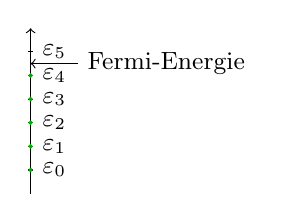
\begin{tikzpicture}[scale=0.3]
      \draw[->] (0,0) -- (0,7);
      \draw (-0.1,1) -- (0.1,1) node[anchor=west]{\small$\varepsilon_0$};
      \draw (-0.1,2) -- (0.1,2) node[anchor=west]{\small$\varepsilon_1$};
      \draw (-0.1,3) -- (0.1,3) node[anchor=west]{\small$\varepsilon_2$};
      \draw (-0.1,4) -- (0.1,4) node[anchor=west]{\small$\varepsilon_3$};
      \draw (-0.1,5) -- (0.1,5) node[anchor=west]{\small$\varepsilon_4$};
      \draw (-0.1,6) -- (0.1,6) node[anchor=west]{\small$\varepsilon_5$};
      \filldraw[green!70!black] (0,1) circle (2pt);
      \filldraw[green!70!black] (0,2) circle (2pt);
      \filldraw[green!70!black] (0,3) circle (2pt);
      \filldraw[green!70!black] (0,4) circle (2pt);
      \filldraw[green!70!black] (0,5) circle (2pt);
      \draw[<-] (0,5.5) -- (2,5.5) node[anchor=west]{\small Fermi-Energie};
    \end{tikzpicture}
    \end{center}
\end{multicols}

Fermi-Temperatur
\begin{equation}
    \theta_F := \frac{\varepsilon_F}{k}\begin{cases}
        T\ll \theta_F \ \text{entartetes Quantengas}\\ T\gg \theta_F \ \text{klass. Grenzfall  } \lambda \ll \left( \frac{V}{N}\right)^{1/3}
    \end{cases}
\end{equation}

\begin{beispiel}{Bsp. Fermionen im 3D-Volumen bei $T \to 0$}
\begin{align}
    N(T=0)&= \int_0^{\varepsilon_F} d\varepsilon\ d(\varepsilon) \\
    d(\varepsilon) &\sim \frac{(2s+1) V\, m^{3/2}}{h^3} \ \sqrt{\varepsilon} \\
    \Rightarrow \ \varepsilon_F &\sim \left(\frac{N}{V}\right)^{2/3}
\end{align}

\begin{equation}
    \left(E_\text{kin} = \varepsilon_F \sim \left(\frac{N}{V} \right)^{2/3}, \ \ E-\text{Coulomb} \sim \frac{1}{r} \sim \left(\frac{N}{V}\right)^{1/3} \right)
\end{equation}
 Energie pro Teilchen:
 \begin{equation}
     \frac{U}{N} = \frac{\int_{-\infty}^{\varepsilon_F} d\varepsilon \ \varepsilon \  d(\varepsilon)}{\int_{-\infty}^{\varepsilon_F} d\varepsilon \  d(\varepsilon)} = \frac{\int_{0}^{\varepsilon_F} d\varepsilon \ \varepsilon^{3/2}}{\int_{0}^{\varepsilon_F} d\varepsilon \  \varepsilon^{1/2}} = \frac{3}{5 } \varepsilon_F
 \end{equation}


    Fermi-Druck

    \begin{equation}
        p \sim \left( \frac{N}{V}\right) ^{5/3}
    \end{equation}
\end{beispiel}

\subsubsection{Tiefe Temperaturen $ T\ll \Theta_F=: \frac{\varepsilon_F}{k}$}

Ziel: Wärmekapazität $C_V$
\begin{equation}
    c_V = \left({\frac{\partial U}{\partial T}}\right)_{V,N} \ \text{z.B. Metallelektronen}
\end{equation}
\begin{itemize}
    \item[Problem:] Großkanonisches Ensemble hat kein festes $N$
    \item[Lösung:] im thermodynamischen Limes gilt: $\underbrace{\expval{N}}_{\text{großkan.}} = \underbrace{N}_{\text{kan}}$
    \begin{enumerate}
    \item Bestimme $N(T,V,\mu) \quad \Rightarrow \quad \mu(T,V,N)$
    \item Bestimme $U(T,V,\mu) \quad \stackrel{\text{elimin. } \mu}{\Longrightarrow}\quad U(T,V,N)$
    \item $C_V$
    \end{enumerate} 
\end{itemize}

\paragraph{1a)} Bestimme $N(T,V,\mu)$ im großkanonischen Ensemble
\begin{itemize}
    \item[$T>0$:] Zustände oberhalb von $\mu$ besetzt
    \item[] Zustände unterhalb von $\mu$ geleert
    \begin{center}
        \begin{tikzpicture}
            \draw[thick,->] (0,-0.1) -- (0,3) node[anchor=south east]{$f(\varepsilon)$};
            \draw[thick,->] (-0.1,0) -- (8,0) node[anchor=west]{$\varepsilon$};
            \draw (3,2.9) -- (-0.1,2.9) node[anchor=east]{1};
            \draw (3,2.9) -- (3,-0.1) node[anchor=north]{$\mu$};
            \draw[green!70!black] plot [smooth] coordinates{(0,2.9) (2,2.61) (3,1.45) (4,0.29) (8,0.1)};
            \draw (3.2,3.3) node{$T=\SI{0}{\K}$};
            \draw[green!70!black] (6,1) node{$T>0$};
        \end{tikzpicture}
    \end{center}
    \item[] Zustandsdichte $d(\varepsilon)$ steigt i.A.
    \begin{itemize}
        \item[$\Rightarrow$] mehr Zustände oberhalb von $\mu$
        \begin{center}
        \begin{tikzpicture}
            \draw[thick,->] (0,-0.1) -- (0,3) node[anchor=south east]{$d(\varepsilon)$};
            \draw[thick,->] (-0.1,0) -- (6,0) node[anchor=west]{$\varepsilon$};
            \draw[thick] (3,0.1) -- (3,-0.1) node[anchor=north]{$\mu$};
            \draw[blue] plot [smooth] coordinates{(2,1.5) (3,2.4) (4,2.8)};
        \end{tikzpicture}
    \end{center}
        \item[] großkan.: $N(T)$ wächst, $\mu = const.$
        \item[] kan.: $N=const.$, $\mu(T)$ sinkt
    \end{itemize}
\end{itemize}
\subparagraph{Sommerfeld-Entwicklung}
\begin{align}
    N(T,\mu) = \int_{-\infty}^{\infty} d\varepsilon \ d(\varepsilon) \ f(\varepsilon) &= \int_{-\infty}^{\infty} d\varepsilon \ d(\varepsilon) \ \underbrace{f_{T=0}(\varepsilon)}_{=\theta(\mu-\varepsilon)} + \int_{-\infty}^{\infty} d\varepsilon \ d(\varepsilon) \underbrace{\left[ f(\varepsilon) - f_{T=0}(\varepsilon)\right]}_{*}\\
    &= \underbrace{\int_{-\infty}^{\mu} d\varepsilon \ d(\varepsilon)}_{=N(T=0,\mu)} + \int_{-\infty}^{\infty} d\varepsilon \ d(\varepsilon) \left[ f(\varepsilon) - f_{T=0}(\varepsilon)\right]
\end{align}
\begin{itemize}
    \item[$\rightarrow$] zu (*):
    \begin{center}
        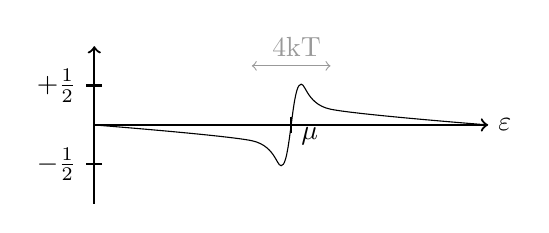
\begin{tikzpicture}
            \draw[thick,->] (0,-1) -- (0,1);
            \draw[thick,->] (0,0) -- (5,0) node[anchor=west]{$\varepsilon$};
            \draw[thick] (0.1,0.5) -- (-0.1,0.5) node[anchor=east]{$+\frac{1}{2}$};
            \draw[thick] (0.1,-0.5) -- (-0.1,-0.5) node[anchor=east]{$-\frac{1}{2}$};
            \draw[thick] (2.5,-0.1) -- (2.5,0.1) node[anchor=north west]{$\mu$};
            \draw plot [smooth] coordinates{(0,0) (2,-0.2) (2.4,-0.5) (2.6,0.5) (3,0.2) (5,0)};
            \draw[black!40,<->] (2,0.75) -- (3,0.75) node[anchor=south east]{4kT};
        \end{tikzpicture}
    \end{center}
    \item[$\rightarrow$] Entwicklung der Zustandsdichte: $d(\varepsilon) = d(\mu) + d^{\prime}(\mu) \cdot (\varepsilon - \mu) + o(\varepsilon^2)$
\end{itemize}

\begin{align}
    N(T,\mu) &= N(T=0,\mu) + d(\mu) \underbrace{\int_{-\infty}^{\infty} d\varepsilon \ [ \underbrace{f(\varepsilon) - f_{T=0}(\varepsilon)}_{\text{ungerade Fkt.}}]}_{=0} + d^{\prime}(\mu) \int_{-\infty}^{\infty} d\varepsilon \ \underbrace{(\varepsilon - \mu) \left[ f(\varepsilon) - f_{T=0}(\varepsilon)\right]}_{\text{gerade Fkt}} + ...\\
    &= N(T=0,\mu) + d^{\prime}(\mu) \cdot \underbrace{2 \cdot \int_{\mu}^{\infty} d\varepsilon \ (\varepsilon - \mu) [ f(\varepsilon) - \underbrace{f_{T=0}(\varepsilon)}_{=0 \text{ für } \varepsilon>\mu}]}_{\stackrel{x = \beta(\varepsilon-\mu)}{=} 2 \cdot (kT)^2 \int_0^{\infty} dx \ \frac{x}{e^x+1} = \frac{1}{2} \zeta(2) = \frac{1}{2} \frac{\pi^2}{6}} + ...
\end{align}

\begin{prop}{Häufige Integrale für Fermi- und Bosegase}
    \begin{align}
        &\int_0^\infty dx \ \frac{x^{t-1}}{e^x +1} = \left(1-\frac{1}{2^{t-1}}\right) \Gamma(t) \zeta(t) \\
        &\int_0^\infty dx \ \frac{x^{t-1}}{e^x -1} =  \Gamma(t) \zeta(t)
    \end{align}
    mit Riemannscher Zeta-Funktion:
    \begin{equation}
        \zeta(t) = \sum_{n=1}^\infty \frac{1}{n^t}
    \end{equation}
\end{prop}
\begin{equation}
    N(T,\mu) = N(T=0,\mu) + \frac{\pi^2}{6}(kT)^2 \, d^{\prime}(\mu) + o((kT)^4)
\end{equation}

\paragraph{1b)} Bestimme $\mu (T)$ bei festem $V,N$:
\begin{align}
    N(T,\mu(T))&= \underbrace{N(T=0,\mu(T))}_{*} + \frac{\pi^2}{6} (k)^2 d^\prime(\mu(T)) + ...\\
    * &=\int_{-\infty}^{\mu(T)} d\varepsilon \ d(\varepsilon) = \underbrace{\int_{-\infty}^{\varepsilon_F} d\varepsilon \ d(\varepsilon)}_{N} + \underbrace{\int_{\varepsilon_F}^{\mu(T)} d\varepsilon \ d(\varepsilon)}_{(\mu(T)-\varepsilon_F) d(\varepsilon_F)}\\
    \Rightarrow \ \ \mu(T)&= \varepsilon_F - \frac{\pi^2}{6} (kT)^2 \frac{d^\prime(\varepsilon_F)}{d(\varepsilon_F)} + o\left( (8kT)^4 \right)
\end{align}

\paragraph{2} ...
\begin{equation}
    U(T) = U(\varepsilon_F) + \frac{\pi^2}{6} \, (kT)^2 \, d(\varepsilon_F) + o\left((kT)^4 \right)
\end{equation}

\paragraph{3}
\begin{equation}
    C_V = \left( \pdv{U}{T} \right)_{V,N} \propto T
\end{equation}
Phononen: $C_V \propto T^3$ \\
Dulong-Petit: $C_V \propto T^0$
\begin{center}
    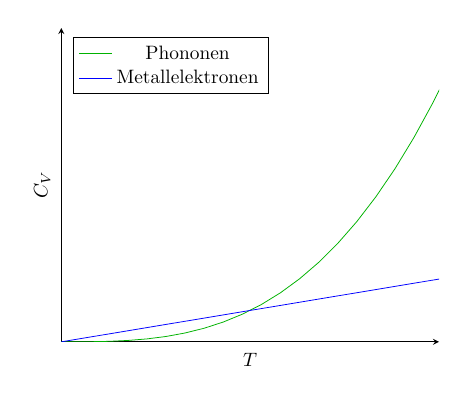
\begin{tikzpicture}[scale=0.7]
        \begin{axis}[axis lines= left,
        ylabel = $C_V$,
        xlabel = $T$,
        xmin = 0 , xmax = 2,
        ymin=0, ymax = 10,
        xtick=\empty,
        ytick=\empty,
        legend pos=north west,]
        \addplot[green!70!black,samples=100]{x^3};
        \addlegendentry{Phononen},
        \addplot[blue,samples=100]{x};
        \addlegendentry{Metallelektronen};
            
        \end{axis}
    \end{tikzpicture}
\end{center}


\subsection{Bose-Einstein-Kondensation} \marginpar{VL 22}
Bose-Gas mit fester Teilchenzahl $N$\\
Problem: Formel Großkanonisches Ensemble\\
Lösung:\\
Bestimme $\mu(T,\frac{N}{V})$ aus
\begin{align}
    N \overset{th. Lim.}{=} \expval{N} = \sum_k \expval{n_k} = \sum_k \frac{1}{e^{\beta(\varepsilon_k-\mu)}-1}
\end{align}
Bem.:
\begin{align}
    \forall k: \space 0 \leq \expval{n_k} \Leftrightarrow \forall k: \mu < \varepsilon_k \rightarrow \mu < \min_k \varepsilon_k= \varepsilon_0 
\end{align}
System idealer Bosonen in 3D Volumen, nicht relativistisch: $\varepsilon(p)=\frac{p^2}{2m}$\\
Zustandsdichte:
\begin{align}
    d(\varepsilon)=(2s+1) \ 4\pi \sqrt{2} \ \frac{Vm^{\frac{3}{2}}}{h^3} \sqrt{\varepsilon} \ \Theta(\varepsilon) \sim \sqrt{\varepsilon}
\end{align}
period. Randbed. $\Rightarrow \ \varepsilon_0=0$\\
Besetzung Grundzustand :
\begin{align}
    \expval{n_0} \stackrel{\mu=-kT}{=} \frac{1}{e-1} = 0,58
\end{align}
Teilchenzahl
\begin{align}
    N &= \sum_k \frac{1}{e^{\beta(\varepsilon_k-\mu)}-1}
    =\int_0^{\infty} d\varepsilon \ d(\varepsilon) \frac{1}{e^{\beta(\varepsilon_k-\mu)}-1}\\
    &\overset{x=\beta\varepsilon}{=} (2s+1) \frac{2}{\sqrt{\pi}}\frac{V}{\lambda^3} I(z)
    \label{eq:BEK}
\end{align}
\begin{itemize}
    \item exakt: wenn $d(\varepsilon) = \sum_k \delta(\varepsilon-\varepsilon_k)$
    \item Näherung: wenn geglättetes $\Bar{d}(\varepsilon) \propto \sqrt{\varepsilon}$
\end{itemize}
\begin{align}
    \text{mit } \lambda=\frac{h}{\sqrt{2\pi mkt}}, \quad I(z) = \int_0^{\infty} dx \ \frac{\sqrt{x}}{\frac{e^x}{z}-1}\\
    \text{außerdem } z=e^{\beta \mu} \ \text{(Fugazität) mit } \mu < 0 \Rightarrow z\in [0,1[
\end{align}
Wie sieht $I(z)$ aus?
\begin{align}
    I(z)= \Gamma\left(\frac{3}{2}\right) Li_{\frac{3}{2}}(z) \text{ mit polylog. } Li_S(z)=\sum_{n=1}^\infty \frac{z^n}{n^S}
\end{align}
Maximalwert bei $z=1$:
\begin{align}
    Li_S(z)=\zeta(S) \ \Rightarrow I(z=1)=\Gamma\left(\frac{3}{2}\right) \zeta\left(\frac{3}{2}\right) \approx 2,3
\end{align}
\begin{center}
    \begin{tikzpicture}[scale=0.5]
        \draw[thick,->] (-0.1,0) -- (5,0) node[anchor=west]{z};
        \draw[thick,->] (0,-0.1) -- (0,3) node[anchor=east]{I(z)};
        \draw[thick] (0.1,2.3) -- (-0.1,2.3) node[anchor=east]{2.3};
        \draw[thick] (1,0.1) -- (1,-0.1) node[anchor=north]{0};
        \draw[thick] (4,0.1) -- (4,-0.1) node[anchor=north]{1};
        \draw plot [smooth] coordinates{(1,0) (3,1.15) (4,2.3)};
        \filldraw (1,0) circle (2pt);
        \filldraw (4,2.3) circle (2pt);
    \end{tikzpicture}
\end{center}
$\Rightarrow$ maximale Teilchenzahl im Limes $\mu \rightarrow 0^- \ (z \rightarrow 1)$
\begin{align}
    N_c(T,V) = (2s+1) \ \zeta\left(\frac{3}{2}\right) \frac{V}{\lambda^3}
\end{align}
Bem.:\\
Dieses $N_c$ entspricht  (bis auf Faktoren) dem Übergang:\\
\begin{center}
    \begin{tabular}{ccc}
    klass. Grenzfall & $\longleftrightarrow$ & Quantengas\\
    $N << N_c$ &  & $N \overset{\approx}{>} N_c$\\
\end{tabular}
\end{center}

$\Rightarrow$ kritische de-Broglie Wellenlänge
\begin{align}
    \lambda_c\left(\frac{N}{V}\right) = \left((2s+1) \zeta\left(\frac{3}{2}\right) \frac{V}{N}\right)^{\frac{1}{3}}
\end{align}
$\Rightarrow$ kritische Temperatur $T_c$ (Bose-Temp.)
\begin{align}
    T_c\left(\frac{N}{V}\right) = \frac{h^3}{2\pi mk} \left((2s+1) \zeta\left(\frac{3}{2}\right) \frac{V}{N}\right)^{-\frac{2}{3}}
\end{align}
Bem.: eliminiere $V$ $\frac{N}{N_C}=\left(\frac{T}{T_C}\right)^{\frac{3}{2}}$ (für später)\\
Für $N>N_c$ oder $T< T_c$ gibt es kein $\mu,z$, so dass \ref{eq:BEK} erfüllt ist.\\
Eigenschaften von:
\begin{align}
    N = \sum_k \frac{1}{e^{\beta(\varepsilon_k-\mu)}-1} = \sum_k \frac{1}{\frac{e^{\beta \varepsilon_k}}{z}-1}
\end{align}
\begin{itemize}
    \item alle Terme $>0$
    \item Terme monoton abfallend für wachsende  $\varepsilon_k$
    \item Größter Beitrag individueller Beitrag für $ \varepsilon_0$ (hier $\varepsilon_0=0$)
        \begin{align}
            \expval{n_0}=\frac{1}{\frac{1}{z}-1}= \frac{z}{1-z} \ \overset{z \rightarrow 1}{\rightarrow} \infty
        \end{align}
        \begin{itemize}
            \item beliebig groß. makroskopische Werte $O(N)$ möglich !
            \item dieser Beitrag fehlt im Integral, da $\Bar{d}(\varepsilon=0)=0$
        \end{itemize}
    \item Man kann zeigen, weitere individuelle Beiträge $\expval{n_k} << \expval{n_0}$
\end{itemize}
\begin{align}
    \Rightarrow N= \sum_k \frac{1}{e^{\beta(\varepsilon_k-\mu)}-1} = \expval{n_0} + \int_0^\infty d\varepsilon \ d(\varepsilon) \frac{1}{e^{\beta(\varepsilon-\mu)}-1}
\end{align}
Für $T<T_c$ ist $\expval{n_0}=N-N_c= O(N)$ makroskopisch\\
\begin{align}
    &\Rightarrow \expval{n_0} = \frac{1}{e^{-\beta\mu)}-1} \approx -\frac{1}{\beta\mu}\\
    &\Rightarrow \mu \approx -\frac{kT}{\expval{n_0}} \text{ ist extrem klein}\\
    &\Rightarrow \mu \to 0 \qq{bzw.} z \to 1
\end{align}
$\Rightarrow$ Im Integral $\mu = 0$ setzen $\Rightarrow$ $z=1$
\begin{align}
    \fcolorbox{red}{white}{\large$N=\expval{n_0} + N_c(T,V)$}
\end{align}
\begin{itemize}
\item[]$T= const$: $N>N_C$ werde erhöht $\Rightarrow$ alle weiteren Bosonen gehen in den Grundzustand, exp. wichtiger:
\item[]$N=const$: $T<T_c$ werdem erniedrigt $\Rightarrow$ $N_c=N\left(\frac{T}{k}\right)^{\frac{3}{2}}$ sinkt $\Rightarrow$ $\expval{n_0}$ wächst
\begin{align}
    \expval{n_0}=N-N_c = N\left[1-\left(\frac{T}{T_c}\right)^{\frac{3}{2}}\right]
\end{align}
\end{itemize}
\begin{center}
    \begin{tikzpicture}[scale=0.6]
        \begin{axis}[
        axis lines = left,
        ylabel={$\frac{\expval{n_0}}{N}$},
        xlabel={$\frac{T}{T_C}$},
        ytick={1},
        xtick={1},
        xmin=0, xmax=1.5,
        ymin=0, ymax=1.2,
        ]
        \addplot[domain=0:1]{1-x^(3/2)};
        \addplot[blue,domain=0:1]{x^(3/2)};
        \addplot[blue,domain=1:1.5]{1};
        \end{axis}
        \draw[blue] (3,5) node[anchor=west]{\tiny Teilchen im angeregten Zustand};
    \end{tikzpicture}
\end{center}
\begin{definition}{Bose-Einstein-Kondensation}
    makroskopisches Quantenphänomen,
    Phasenübergang: bei $T<T_c$ existieren 2 Phasen
    \begin{itemize}
        \item $\expval{n_0}$ Teilchen im Grundzustand
        \item $N-\expval{n_0}$ Teilchen im angeregten Zuständen
        \item Phasen räumlich nicht getrennt (nur bei flüssig/gasförmig)
    \end{itemize}
\end{definition}
\textbf{Bem.:} Wenn $T$ klein genug $\Rightarrow$ alle Teilchen im Grundzustand nach klass. Maxwell-Boltzmann-Statistik
\begin{align}
    \frac{\expval{n_0}}{\expval{n_1}} = \frac{e^{-\beta \varepsilon_0}}{e^{-\beta \varepsilon_1}}=e^{\beta(\varepsilon_1-\varepsilon_0)} >> 1 \text{ für kleine }T
\end{align}
Bei welchen T?
\begin{align}
    kT << \varepsilon_1-\varepsilon_0 = \frac{\hbar^2(\Delta k)^2}{2m} = \frac{\hbar^2}{2m}\left(\frac{2\pi}{L}\right)^2 = \frac{\hbar^2}{2m}\left(\frac{1}{V}\right)^{\frac{2}{3}} \widehat{=} \lambda \gg V^{\frac{1}{3}}
\end{align}
Zum Vergleich $T_c$ BEC:
\begin{align}
    kT_c = \frac{\hbar^2}{m}\left(\frac{N}{V}\right)^{\frac{2}{3}} \widehat{=} \lambda \approx V^{\frac{1}{3}}
\end{align}
$\Rightarrow$ BEC bereits bei um $N^{\frac{2}{3}}$ höheren Temperaturen \\
Ursache: Bose-Einstein-Statistik für identische quantenmechanische Teilchen

\paragraph{Experiment:}
\begin{itemize}
    \item Problem: hier nur ideales Bose-Gas, real: WW
    \item verbundene Phänomene:
    \begin{itemize}
        \item Supraleitung (Cooper-Paare)
        \item Superfluidität ($^4 He$)
    \end{itemize}
    \item[$\Rightarrow$] experimentelle Umsetzung: weniger WW $\rightarrow$ Gas
    \begin{itemize}
        \item niedrige Temperatur $\rightarrow$ Verflüssigung
        \begin{itemize}
            \item[$\Rightarrow$] Lösung: verdünntes Gas 
        \end{itemize}
    \end{itemize}
    \item[$\Rightarrow$] erstmals 1995 gelungen, 2001 Nobelpreis
    \item[$\Rightarrow$] $10^{-6} \si{\K} = T$ notwendig
\end{itemize}

\subsection{Photonengas}\marginpar{VL 23}
\begin{wrapfigure}{l}{0.2\textwidth}
   \begin{tikzpicture}
    \coordinate (x1) at (0,0);
    \coordinate (x2) at (1,0);
    \coordinate (y1) at (0,1);
    \coordinate (y2) at (1,1);
    \draw (x1) to[out=-90,in=-180] (x2) to[out=-90,in=30] (y2) to[out=-90,in=-30] (y1) to[out=180,in=30] (x1);
\end{tikzpicture} 
\end{wrapfigure}
Elektromagnetische Strahlung im Gleichgewicht mit Hohlraumwand \\ $\Rightarrow$ Maxwell Gleichungen $\rightarrow$ lineare Superposition von monochromatischen Eigenzuständen. \\ Eigenmoden:
\begin{itemize}
    \item durch Form und Randbedingungen festgelegt
    \item sehen i.A. irregulär aus
    \item hier nur mittlere Dichte der Eigenfrequenzen wichtig
\end{itemize}
Zustandsdichte (siehe \cref{abs.Kontinuumslimes})
\begin{itemize}
    \item in $k = \abs{\Vec{k}}$:
    \begin{equation}
        d(k) = \underbrace{2}_{\substack{Maxwell-Gl: \\ \Vec{E},\Vec{B} \perp \Vec{k}}} \cdot \left(\frac{L}{2\pi}\right)^3 \cdot \underbrace{\overbrace{4\pi k^2}^{\text{\tiny Oberfläche}} \cdot dk}_{\text{\tiny Kugelschale}} = \frac{V}{\pi^2} k^2 \, dk
    \end{equation}
    \item in $\omega = ck$:
    \begin{equation}
        d(\omega) \, d\omega = \frac{V}{\pi^2c^3} \omega^2 \, d\omega
    \end{equation}
    \item in $\varepsilon=\hbar \omega$:
    \begin{equation}
        d(\varepsilon) \, d\varepsilon = \frac{V}{\pi^2\hbar^3c^3} \varepsilon^2\, d\varepsilon
    \end{equation}
    \item[] \color{black!40} Man nutzt hier die Multipikation mit dem Differential, um eine dimensionslose Größe zu erzeugen und damit die Ausdrücke auf der linken Seite gleichsetzen zu können. Es gilt dann:
    \begin{equation}
         d(x) \, dx = d(x(y)) \dv{x}{y} \, dy
    \end{equation}
    \begin{itemize}\color{black}
        \item[$\rightarrow$] klassische ED: Amplitude der Eigenmode $k$ kontinuierlich
        \item[] QED: Qunatisierung der mode analog zum H.O.:
        \begin{align}
            \varepsilon_n &= \hbar \omega(k) \left(\frac{1}{2}+n\right) \qquad n=0,1,2,...\\
            &\Rightarrow n \qq{Photonen (Bosonen) im Einteilchenzustand mit Energie $\hbar \omega$}
        \end{align}
    \end{itemize}
\end{itemize}

\paragraph{statistiscche Eigenschaften der Photonen} (wichtig für Besetzung $n_k$)
\begin{itemize}
    \item Spin = 1 $\Rightarrow$ Bosonen
    \item keine WW $\Rightarrow$ ideales Bosegas
    \item ABER: Anzahl der Photonen ist keine Erhaltungsgröße (ständige Absorption/Emission der Photonen an Wand)
    \begin{equation}
        \varrho = \frac{1}{Z} e^{-\beta H} \qq{mit beliebiger Teilchenzahl}
    \end{equation}
    \begin{itemize}
        \item[] vgl. mit großkanonischem Ensemble: \fcolorbox{green!70!black}{white}{$\mu = 0$} für Photonen
        \begin{equation}
            \Rightarrow \qq{mittlere Besetzungszahl:} \expval{n_k} = \frac{1}{e^{\beta \varepsilon_k}-1}
        \end{equation}
    \end{itemize}
\end{itemize}

\subsubsection{Planck'sches Strahlungsgesetz}
\begin{equation*}
    \qq{spektrale Energiedichte} = \frac{\text{Energie}}{\text{Volumen}\cdot \text{Energieintervall}}
\end{equation*}
\begin{align}
    \varrho(\varepsilon,T) \, d\varepsilon &= \frac{1}{V} \cdot d(\varepsilon) \cdot \expval{n_{\varepsilon}} \cdot \varepsilon \, d\varepsilon\\
    &= \frac{1}{V} \cdot \frac{V}{\pi^2\hbar^3c^3}\varepsilon^2 \cdot \frac{1}{e^{\beta\varepsilon}-1}\cdot \varepsilon \, d\varepsilon\\
    &= \frac{\varepsilon^3 \, d\varepsilon}{\pi^2\hbar^3c^3\left(e^{\beta \varepsilon}-1\right)}
\end{align}
in $\omega\quad(\varepsilon=\hbar\omega)$:
\begin{align}
    \fcolorbox{red}{white}{$\varrho(\omega,T) \, d\omega = \frac{\hbar}{\pi^2c^3}\frac{\omega^3}{e^{\frac{\hbar\omega}{kT}}-1}\,d\omega$} \quad \text{Planck'sches Strahlungsgesetz (1900)}
\end{align}

\begin{center}
    \begin{tikzpicture}
        \begin{axis}[
        axis lines=left,
        xlabel={$\omega$},
        ylabel={$\varrho(\omega)$},
        xmin=0, xmax=0.5,
        ymin=0, ymax=5.5,
        xtick=\empty,
        ytick=\empty,
        ]
        \addplot[color=blue, samples=100,domain=0:0.5]{100000*(x^3)/(e^(30*x)-1)};
        \addplot[color=red, samples=100,domain=0:0.5]{100000*(x^3)/(e^(40*x)-1)};
        \end{axis}
        \draw[->] (0.75,1) -- (1.25,3) node[anchor=south west]{T};
    \end{tikzpicture}
\end{center}
\begin{itemize}
\item dimensionslos:
\begin{align}
    x &= \frac{\hbar\omega}{kT} \qquad \Tilde{\varrho}:= \varrho \frac{1}{kT} \left(\frac{\hbar c}{kT}\right)^3\\
    &\Rightarrow \Tilde{\varrho}(x) \, dx = \frac{1}{\pi^2} \frac{x^3}{e^x-1} \, dx
\end{align}
\item[]$\rightarrow$ Daraus ist erkennbar, dass es sich im Diagramm oben um die gleichen Kurven handelt, diese lediglich anders skalieren:
\begin{equation*}
    \omega \rightarrow \frac{\omega}{T} \qq{,} \varrho \rightarrow \frac{\varrho}{T^3}
\end{equation*}
\item Maximum:
\begin{equation}
    \dv{\varrho(\omega,T)}{\omega}\stackrel{!}{=} 0 \quad \Rightarrow \quad \omega_{\text{max}} \approx 2.82 \frac{kT}{\hbar} \propto T \qq{(Wien'sches Verschiebungsgesetz)}
\end{equation}
\item Grenzfälle:
\begin{itemize}
    \item $\hbar\omega \ll kT$:
    \begin{equation}
        \varrho(\omega,T) \approx \frac{\omega^2kT}{\pi^2c^3} \qq{(Rayleigh-Jeans-Gesetz)}
    \end{equation}
    \item $\hbar\omega \gg kT$:
    \begin{equation}
        \varrho(\omega,T) \approx \frac{\hbar\omega^3}{\pi^2c^3} e^{-\frac{\hbar\omega}{kT}} \qq{(Wien)}
    \end{equation}
\end{itemize}
\end{itemize}

\paragraph{Energiedichte} $\left(\frac{\text{Energie}}{\text{Volumen}}\right)$
\begin{align}
    u(T) &= \frac{U}{V}= \int_0^{\infty} \varrho(\omega,T) \, d\omega = \frac{\hbar}{\pi^2 c^3}\, \int_0^{\infty} \, d\omega \ \frac{\omega^3}{e^{\frac{\hbar\omega}{kT}}-1}\\
    &\stackrel{x=\frac{\hbar\omega}{kT}}{=} \frac{(kT)^4}{\pi^2c^3\hbar^3} \underbrace{\int_0^{\infty} \, dx \ \frac{x^3}{e^x-1}}_{=\Gamma(4)\zeta(4) = 3! \frac{\pi^4}{90}=\frac{\pi^4}{15}} = \frac{\pi^2(kT)^4}{15 (\hbar c)^3} \propto T^4
\end{align}
\paragraph{Strahlungsdichte} $\left(\frac{\text{Energie}}{\text{Fläche}\cdot\text{Zeit}}\right)$
\begin{center}
\begin{tikzpicture}
    \coordinate (c) at (3,0);
    \draw (c) ellipse (0.5cm and 1cm);
    \draw (c) ellipse (0.3cm and 0.6cm);
    \draw (0,-1)--(0,1);
    \draw[dashed] (0,0)--(c);
    \draw (0,0)--(3,0.6cm);
    \draw (0,0.4cm)--(3,1cm) node[midway,above] {$c dt$};
    \draw[ultra thick, green!50!black] (0,0) -- (0,0.4cm) node[midway, left]{$dA$};
    \draw (3.8,0) node{$\varphi$};
    \draw (1.5,0) arc (0:11:1.5);
    \draw (1,0.1) -- (1,-0.5) node[anchor=north]{$\vartheta$}
\end{tikzpicture}
\end{center}
\begin{align}
    j(T) \,dt\,dA &= u(T) \frac{1}{4\pi} \int_0^{2\pi} \,d\varphi \ \underbrace{\int_0^{\frac{\pi}{2}} \, d\vartheta \ \sin(\vartheta) c \,dt\, \cos(\vartheta)\,dA}_{=\frac{1}{2} c \,dt\,dA} \\
    &\Rightarrow \quad \fcolorbox{red}{white}{$j(T)=\sigma \cdot T^4$} \qq{mit} \sigma = \frac{\pi^2}{60} \frac{k^4}{\hbar^3c^2} \qq{(Stefan-Boltzmann-Gesetz)}
\end{align}

\paragraph{Großkanonisches Potential:}
\begin{align}
    \Phi &= - p \cdot V\\
    \Phi &= -kT \ln(Z_G) = ... = -\frac{V}{3} u(T)
\end{align}
\begin{itemize}
    \item[$\Rightarrow$] Strahlungsdruck:
    \begin{equation}
        p = \frac{1}{3} u(T) \qquad \color{black!40}\left(\text{siehe Übung 12.2: } p = \frac{n}{d}u\right)
    \end{equation}
    \item[$\Rightarrow$] Entropie:
    \begin{align}
        S = - \left(\pdv{\Phi}{T}\right)_{V,\mu} &= \frac{V}{3} \cdot 4 \cdot \frac{u(T)}{T}\\
        &\Rightarrow \quad U = \frac{3}{4} ST
    \end{align}
\end{itemize}

\begin{beispiel}{Beispiel: kosmische Hintergrundstrahlung}
    \begin{itemize}
        \item[] Urknall: Materie und Strahlung im Gleichgewicht
        \item[] $\Rightarrow$ Zeitpunkt der Bildung von Atomen: Trennung von Materie und Strahlung etwa bei Temperatur \SI{3000}{\K}
        \begin{itemize}
            \item[$\rightarrow$] danach: keine Änderung der Verteilung ($\varrho(\omega,T)$) mehr
            \item[$\rightarrow$] Volumen Universum: Faktor 1000
            \item[$\rightarrow$] Temperatur Universum: Faktor $\frac{1}{1000}\quad \Rightarrow$ \SI{3}{\K}
        \end{itemize}
    \end{itemize}
\end{beispiel}



\subsection{Phononengas}\marginpar{VL 24}
Ziel: Beitrag der Gitterschwingungen zur Wärmekapazität von Festkörpern (Metallelektronen $\rightarrow$ Fermi-Gas $\rightarrow$ $C_V\sim T$)\\
\newline
\paragraph{1 D Gitter der Atome:}
\begin{center}
    \begin{tikzpicture}
        \draw[thick] (0,0) -- (11,0);
        \foreach \x in {1,2,3,4,5,6,7,8,9,10}{
            \filldraw[blue] (\x,0) circle (2pt);
            \draw[thick] (\x,1) -- (\x,0.6);
        }
        \foreach \x in {1,2,3,4,5,6,7,8,9,10,11}
            \draw[decoration={aspect=0.3, segment length=3pt, amplitude=2pt,coil},decorate] (\x-1,0.8) -- (\x,0.8);
        \draw[thick] (9,1.3) -- (9,1.5);
        \draw[thick] (9,1.4) -- (10,1.4) node[midway,above]{a};
        \draw[thick] (10,1.3) -- (10,1.5);
        \filldraw[black!40] (4.4,0) circle (2pt);
        \draw[->, black!40] (4,-0.3) -- (4.4,-0.3) node[midway,below]{$u_\nu(t)$};
    \end{tikzpicture}
\end{center}
Potentielle Energie:
\begin{align}
    V=V_0+\sum_{\nu =1}^N \frac{K}{2} (u_\nu-u_{\nu+1})^2 \qquad \qquad (\text{per. RB: }U_{N+1}=U_1)
\end{align}
Bewegungsgleichung für Atom j:
\begin{align}
    \ln \pdv[2]{u_j}{t} &= - \pdv{u_j} V = -K(u_j - u_{j+1})-K(u_{j-1}-u_j)\\
    &= -K(2u_j-u_{j+1}-u_{j-1})
\end{align}
N gekoppelte DGL 2.Ordnung
\subparagraph{1. Ansatz Ebene Welle:}
\begin{align}
    u_j^k(t)=Ae^{i(jka-\omega (k) t)}
\end{align}
Einsetzen:
\begin{align}
    -m\omega^2(k)=-K(2-e^{ika}-e^{-ika})=-2K\underbrace{(1-cos(ka))}_{2\sin^2(\frac{ka}{2})}
\end{align}
\begin{align}
    \Rightarrow \ \omega (k) = \underbrace{\pm}_{\text{keine neue Lsg}} 2\sqrt{\frac{K}{m}}\abs{\sin{\frac{ka}{2}}}
\end{align}
reelle Lösung:
\begin{align}
    u_j^k(t)=A\cos{(kja-\omega (k)t)}
\end{align}
erlaubte k-Werte aus RB:
\begin{align}
    u_{N+1}=u_1 \ \Rightarrow e^{ikNa}=1 \ \Rightarrow k=\frac{2\pi n}{aN}, n \in \mathbb{Z}
\end{align}
\begin{align}
    k'=k+\frac{2\pi}{a} \qq{ist eine Lsg}\\
    \Rightarrow \text{wähle }k\in \left[-\frac{\pi}{a},\frac{\pi}{a}\right) \Rightarrow N\text{ Eigenmoden}
\end{align}
Dispersionsrelation:
\begin{center}
    \begin{tikzpicture}[scale=0.8]
        \begin{axis}[
        axis x line=center,
        axis y line=center,
        xlabel= $k$,
        ylabel=$\omega(k)$,
        xmin=-3.2,xmax=3.2,
        ymin=0,ymax=1.1,
        xtick={-3.14,3.14},
        ytick={1},
        xticklabels={$-\frac{\pi}{a}$, $\frac{\pi}{a}$}
        ]
        \addplot[color=blue, samples=100, domain=0:3.141]{sin(deg(x/2))};
        \addplot[color=blue, samples=100, domain=-3.141:0]{-sin(deg(x/2))};
        \end{axis}
    \end{tikzpicture}
\end{center}
$\abs{k}<<\frac{\pi}{a}$:
\begin{align}
    \omega (k)= 2\sqrt{\frac{K}{m}}\abs{\frac{ka}{2}} = \underbrace{\sqrt{\frac{K}{m}} a}_{=c_s \text{ Schallgeschw.(akustische Mode)}} \abs{k}
\end{align}

\subparagraph{2. Ansatz Normalkoordinaten:}
\begin{align}
    \xi^k(t):=\sum_{j=1}^Ne^{-ikja} u_j(t)
\end{align}
entkoppeln DGK für jedes $k=\frac{2\pi n}{aN}$:
\begin{align}
    \dv[2]{}{t}\xi^k(t)=-\omega^2(k)\xi^k(t)
\end{align}
$\Rightarrow$ N harm. Osz. mit Frequenz $\omega(k)$\\
$\longrightarrow$ Quantisierung der Normalschwingung:
Energien
\begin{align}
    E_k=\hbar\omega (k) \left(\frac{1}{2} + n_k\right) = \frac{1}{2} \hbar \omega (k) + n_k \underbrace{ \hbar\omega (k)}_{\varepsilon_k}
\end{align}
$\Rightarrow$ analoge Beschreibung: $n_k$ Phononen mit Energie $\varepsilon_k$\\
$\widehat{=}$ ideales Bose-Gas:\\
$\mu = 0$ (Wie bei Photonen)\\
\begin{align}
    \expval{n_k}=\frac{1}{e^{\beta \varepsilon_k}-1}
\end{align}

\paragraph{Realer Festkörper}
\subparagraph{3D:}
$\left. 
  \begin{array}{ c l }
    N & \quad \text{longitudinale Moden} \\
    +2N  & \quad \text{transversale Moden}
  \end{array}
\right\}$ $3N$ Moden\\

\begin{center}
    \begin{tikzpicture}[scale=0.8]
        \begin{axis}[
        axis x line=center,
        axis y line=center,
        xlabel= $k$,
        ylabel=$\omega(k)$,
        xmin=-3.2,xmax=3.2,
        ymin=0,ymax=1.4,
        xtick={-3.14,3.14},
        ytick={1},
        xticklabels={$-\frac{\pi}{a}$, $\frac{\pi}{a}$}
        ]
        \addplot[color=blue, samples=100, domain=0:3.141]{sin(deg(x/2))};
        \addplot[color=blue, samples=100, domain=-3.141:0]{-sin(deg(x/2))};
        \addplot[color=green!70!black, samples=100, domain=0:3.141]{1.2*sin(deg(x/2))};
        \addplot[color=green!70!black, samples=100, domain=-3.141:0]{-1.2*sin(deg(x/2))};
        \end{axis}
        \draw[blue] (7,4) node[anchor=west]{longitudinal};
        \draw[green!70!black] (7,5) node[anchor=west]{(2$\times$) transversal };
    \end{tikzpicture}
\end{center}

\subparagraph{1D 2 Atome per Einheitszelle:}
\begin{center}
    \begin{tikzpicture}[scale=0.8]
        \begin{axis}[
        axis x line=center,
        axis y line=center,
        xlabel= $k$,
        ylabel=$\omega(k)$,
        xmin=-3.2,xmax=3.2,
        ymin=0,ymax=2,
        xtick={-3.14,3.14},
        ytick={1},
        xticklabels={$-\frac{\pi}{a}$, $\frac{\pi}{a}$}
        ]
        \addplot[color=blue, samples=100, domain=0:3.141]{sin(deg(x/2))};
        \addplot[color=blue, samples=100, domain=-3.141:0]{-sin(deg(x/2))};
        \addplot[color=green!70!black, samples=100, domain=-3.141:3.141]{0.2*cos(deg(x))+1.5};
        \end{axis}
        \draw[blue] (7,2.9) node[anchor=west]{akustischer Zweig};
        \draw[green!70!black] (7,3.8) node[anchor=west]{optischer Zweig};
    \end{tikzpicture}
\end{center}

\subparagraph{3D p Atome per Einheitszelle:}
\begin{itemize}
    \item $3$ akust. Zweige mit $3N$ akust. Moden
    \item $3(p-1)$ opt. Zweige mit $3N(p-1)$ opt. Moden
\end{itemize}

\paragraph{Statistische Physik}

Innere Energie
\begin{align}
    U=U_0+ \sum_k \expval{n_k} \varepsilon_k = U_0 + \sum_k \frac{\varepsilon_k}{e^{\beta \varepsilon_k}-1} \qquad k=(\Vec{k},\underbrace{s}_{\text{Zweige}})
\end{align}
Wärmekapazität
\begin{align}
    c_V=\left( \pdv{U}{T}\right)_V = \sum \frac{\varepsilon_k (-1) e^{\beta\varepsilon_k}\varepsilon_k \frac{-1}{k_BT^2}}{(e^{\beta \varepsilon_k}-1)^2} = k_B \sum_k \frac{(\beta\varepsilon_k)^2e^{\beta \varepsilon_k}}{(e^{\beta \varepsilon_k}-1)^2}
\end{align}
\begin{enumerate}
    \item hohe Temperaturen $k_B T>>\max_k \varepsilon_k$
        \begin{align}
            &\Rightarrow \beta\varepsilon_k << 1 \Rightarrow e^{\beta\varepsilon_k}=1+\beta\varepsilon + ...\\
            &\Rightarrow c_V = k_B\sum \frac{(\beta\varepsilon_k)^2}{(\beta\varepsilon_k)^2} = k_B \sum_k 1 = 3Nk_B \qq{Dulong-Petit}
        \end{align}
    \item tiefe Temperaturen $k_B T<<\max_k \varepsilon_k$\\
        Nur wenige Beiträge mit $\varepsilon_k \leq k_BT$ wichtig\\
        $\Rightarrow$ nur wenige akustische Zweige $(s=1,2,3)$ mit $\omega(k)=c_S(\Vec{k})\abs{\Vec{k}}$
        \begin{align}
            \sum_k &\rightarrow \underbrace{3}_{\text{Zahl der Zweige}}\underbrace{\frac{1}{\left(\frac{2\pi}{L}\right)^2}}_{\text{Volumen Zelle in k-Raum}}\int_0^{k_{\max}}dk \ 4\pi k^2\\
            c_V &= k_B \frac{12\pi V}{8 \pi^3} \int_0^{k_{\max}} dk \ k^2 \frac{(\beta \hbar ck)^2 e^{\beta \hbar ck}}{(e^{\beta \hbar ck}-1)^2}\\
            &\overset{x=\beta \hbar ck}{=} \frac{3Vk_B}{2\pi^2} \left(\frac{k_BT}{\hbar c}\right)^3 \underbrace{\int_0^{\beta\hbar ck_{\max}\to \infty}dx \frac{x^4 e^x}{(e^x-1)^2}}\\
            &\qquad \stackrel{p.I.}{=} ... \underbrace{\left[x^4 \frac{-1}{e^x-1}\right]_0^\infty}_{=0} + \underbrace{\int_0^\infty dx \ \frac{4 x^3}{e^x-1}}_{=4 \Gamma(4)\zeta(4) = \frac{\pi^4}{15}}\\
            c_V &=\frac{2\pi^2Vk_B}{5} \left(\frac{k_BT}{\hbar c}\right)^3 \sim T^3
        \end{align}
        \begin{center}
        \begin{tikzpicture}[scale=0.8]
            \draw[thick,->] (0,-0.1) -- (0,4) node[anchor=east]{$c_V$};
            \draw[thick,->] (-0.1,0) -- (2.5,0) node[anchor=west]{$T$};
            \draw[green!70!black] plot [smooth] coordinates{(0,0) (0.25,0.0078125) (0.5,0.0625) (0.75,0.2109375) (1,0.5) (1.5,1.6875) (2,4)} node[anchor=east]{\tiny Phononen};
            \draw[blue] (0,0) -- (2,2) node[anchor=south]{\tiny$e^-$};
        \end{tikzpicture}
        \end{center}
        \item allgemein: Debye-Modell
        \begin{itemize}
            \item akustische Zweige mit $\omega=c_D \abs{\Vec{k}}$
            \item Bestimmung von $k_{max} = k_D$
        \end{itemize}
\end{enumerate}
\begin{align}
    \underbrace{\sum_k 1}_{3D} &= 3 \left(\frac{L}{2\pi}\right)^3 \underbrace{4\pi \int_0^{k_{\text{max}}=k_D} dk \, k^2}_{=\frac{4\pi}{3}k_D^3} \\
    &\Rightarrow k_D = \left(6\pi^2\frac{N}{V}\right)^{1/3}\\
    &\Rightarrow c_V = \frac{3 V k_B}{2\pi} \left(\frac{k_B T}{\hbar c}\right)^3 \int_0^{\beta\hbar ck_D}dx \frac{x^4 e^x}{(e^x-1)^2}
\end{align}
\begin{align}
    &\qq{Debye-Frequenz:} \omega_D = c k_D = c k_{max}\\
    &\qq{Debye-Temperatur:} k_B \theta_D = \hbar \omega_D = \hbar c k_D\\
    &\Rightarrow \scalebox{1.1}{\fcolorbox{green!70!black}{white}{$c_V = 9Nk_B \left( \frac{T}{\theta_D}\right)^3 \Big\int_0^{\frac{\theta_D}{T}} dx \frac{x^4 e^x}{(e^x-1)^2}$}}
\end{align}


\begin{center}
        \begin{tikzpicture}[scale=0.8]
            \draw[thick,->] (0,-0.1) -- (0,4) node[anchor=east]{$c_V$};
            \draw[thick,->] (-0.1,0) -- (5,0) node[anchor=west]{$T$};
            \draw[thick] (0.1,3) -- (-0.1,3) node[anchor=east]{$3k_BT$};
            \draw[thick] (1.6,0.1) -- (1.6,-0.1) node[anchor=north]{$\theta_D$};
            \draw[green!70!black] plot [smooth] coordinates{(0,0) (0.25,0.0078125) (0.5,0.0625) (0.75,0.2109375) (1,0.5) (1.5,1.6875) (2,2.4) (2.5,2.8) (3,2.95) (3.5,3) (4,3)};
            \draw (0.4,0.3) node{\tiny$\sim T^3$};
            \draw (3.5,2.8) node{\tiny$\sim T^0$};
        \end{tikzpicture}
\end{center}

\subsection{Wechselwirkende Teilchen} \marginpar{VL 25}
bisher: ideale Gase, d.h. keine WW\\
realistische Systeme: WW oft klein

\subsubsection{Virialentwicklung}
Sei WW kurzreichweitig (z.B. Moleküle eines Gases).
\begin{itemize}
    \item[$\Rightarrow$] bei geringer Dichte $n=\frac{N}{V}$ kleine Störung
    \item[$\rightarrow$] Entwicklung nach kleinen $n$
    \begin{equation}
        \underbrace{\frac{p}{kT} = n}_{\text{ideales Gas}} + \sum_{l=2}^{\infty} \underbrace{B_l(T) \quad n^l}_{\text{Korrektur der Ordnung } l}
    \end{equation}
\end{itemize}

\paragraph{Bemerkung:}
\begin{itemize}
    \item $B_l$ ist $l$-ter Virialkoeffizient
    \item Name wegen Virialsatz: $\expval{E_{kin}} = - \frac{1}{2} \sum_i \expval{\Vec{F}_i\cdot \Vec{r}_i}$
    \item $B_l = B_l(T)$
    \item experimentell werden $B_2(T)$ und $B_3(T)$ bestimmt
\end{itemize}

\paragraph{Frage:} Wie hängen $\underbrace{B_2(T)}_{\text{makroskopisch}}$ mit $\underbrace{\text{WW-Potential } W(\Vec{r})}_{\text{mikroskopisch}}$ zwischen Molekülen zusammen?

\paragraph{Ergebnis:}
\begin{equation}
    \fcolorbox{red}{white}{$B_2(T) = \frac{1}{2} \int_V \, d^3r \ \left(1-e^{-\beta W(\Vec{r})}\right)$}
\end{equation}
\color{black!40} V muss nur WW-Bereich einschließen, da der Integrand sonst annähernd bzw exakt null ist. Daher gibt es keine V Abhängigkeit. \color{black}
\paragraph{Herleitung}
Großkanonische Zustandssumme:
\begin{align}
    Z_G = \Tr\left(e^{-\beta(\hat{H}-\mu \hat{N})}\right) = \sum_{N=0}^{\infty}\underbrace{Z(T,V,N)}_{=: Z_n \text{ kanon.}} e^{\beta\mu N} = \underbrace{Z_0}_{e^{-\beta E_{\text{\tiny Vakuum}}}=1 }+ \sum_{l=1}^{\infty} \, Z_l \, z^l \\
    \qq{mit} z := e^{\beta \mu} \qq{Fugazität} z \ll 1    
\end{align}
Großkanonisches Potential:
\begin{align}
    \Phi &= -pV = -kT \ \ln(Z_G) \\
    &\Rightarrow \frac{pV}{kT} = \ln(Z_G) = \ln\left(1 + \sum_{l=1}^{\infty}\, Z_l \, z^l\right) =: \sum_{l=1}^{\infty}\, a_l \, Z^l \label{4_eq:1_virial} \\
    N &= -\pdv{\Phi}{\mu} = V \pdv{p}{\mu} \stackrel{(\ref{4_eq:1_virial})}{=} V \pdv{p}{z} \underbrace{\pdv{z}{\mu}}_{\beta z} = V \frac{kT}{V} \sum_{l=1}^{\infty} \, a_l \, l \, z^{l-1} \beta z = \sum_{l=1}^{\infty} \, l\,a_l \, z^l \label{4_eq:2_virial}
\end{align}

\subparagraph{1} Bestimme $a_l(Z_1,Z_2,..)$ aus \cref{4_eq:1_virial}:
\begin{align}
    \ln(1+x) &= x - \frac{x^2}{2} + \frac{x^3}{3} -... \qq{mit} x = \sum_{l=1}^{\infty} \, Z_l \, z^l\\
    &\stackrel{\text{bis 2. Ord.}}{=} (Z_1z+Z_2 z^2+..) - \frac{1}{2} (Z_1 z+...)^2 +...\\
    &= \underbrace{Z_1}_{=a_1} + \underbrace{(Z_2 - \frac{1}{2}Z_1^2)}_{= a_2} z^2 + ...
\end{align}

\subparagraph{2} Invertiere \cref{4_eq:2_virial} zu $\sum_{m=1}^{\infty} \, b_m N^m$:
\begin{align}
    (\ref{4_eq:2_virial}): \ N &= 1\cdot a_1 \cdot (b_1N^1+b_2N^2+...)^1 + 2\cdot a_2 \cdot (b_1 N +...)^2 + ...\\
    &= \underbrace{a_1b_1}_{=1}N + \underbrace{(a_2b_2+2a_2b_1^2)}_{=0}N^2+...\\
    &\Rightarrow b_1 = \frac{1}{a_1} \quad b_2 = -\frac{2 a_2b_1^2}{a_1} = -\frac{2a_2}{a_1^3}
\end{align}

\subparagraph{3} Eliminiere damit $z$ in \cref{4_eq:1_virial}:
\begin{align}
    \frac{pV}{kT} &= \sum_{l=1}^{\infty} a_l z^l = a_1(b_1N+b_2N^2+...)+a_2(b_1N+...)^2+...\\
    &= \underbrace{a_1b_1}_{=1} N + \underbrace{(a_1b_2+a_2b_1^2)} N^2 + ...\\
    & - \frac{2a_2}{a_1^2} + \frac{a_2}{a_1^2} = -\frac{a_2}{a_1^2} = - \frac{Z_2 - \frac{1}{2}Z_1^2}{Z_1^2} = \frac{1}{2} - \frac{Z_2}{Z_1^2} \\
    \frac{p}{kT} &= n + \underbrace{V\left(\frac{1}{2}-\frac{Z_2}{Z_1^2}\right)}_{=B_2(T)} n^2+...
\end{align}

\subparagraph{4} Bestimme kanonische Zustandssumme $Z_1,Z_2,...$:
\begin{align}
    &\rightarrow \qq{kline Dichten} n = \frac{N}{V} \qq{im Sinne} \left(\frac{V}{N}\right)^{1/3} \gg \lambda = \frac{h}{\sqrt{2\pi mkT}} \qq{kl. Grenzfall}\\
\end{align}
1 Teilchen:
\begin{align}
    Z_1 &= \frac{1}{h^3} \underbrace{\int d^3q}_{=V} \, \underbrace{\int d^3p \ e^{-\beta \frac{p^2}{2m}} }_{(\sqrt{2\pi mkT})^3} = \frac{V}{\lambda^3} \\
    (\Rightarrow z=b_1N+...&=\frac{1}{a_1}N+...=\frac{1}{Z_1}N+...= \lambda^3 \cdot \frac{N}{V} + ... \ll 1 \Rightarrow z \ll 1 )\\
    &\rightarrow \qq{rechtfertigt Entwicklung in (\ref{4_eq:1_virial}) und (\ref{4_eq:2_virial})}
\end{align}
2 Teilchen:
\begin{align}
    Z_2 &= \frac{1}{2!} \frac{1}{h^6} \int_V d^3q_1 \, \int_V d^3q_2 \, \int d^3p_1 \, \int d^3p_2 e^{-\beta \left(\frac{p_1^2}{2m}+\frac{p_2^2}{2m}+W(\Vec{q}_1 - \Vec{q}_2)\right)} \\
    &W(\Vec{q}_1 - \Vec{q}_2) \qq{Zweiteilchen WW}\\
    &= \frac{1}{2} \frac{(\sqrt{2\pi mkT})^6}{h^6} \underbrace{\int d^3R}_{V} \, \int d^3r \, e^{-\beta W(\Vec{r})} \qq{mit} \Vec{r} = \Vec{q}_1 - \Vec{q}_2, \ \Vec{R} = \frac{\Vec{q}_1 + \Vec{q}_2}{2} \\
    &= \frac{V}{2\lambda^2} \int d^3r e^{-\beta W(\Vec{r})}\\
    &\Longrightarrow B_2(T) = V\left(\frac{1}{2}-\frac{Z_2}{Z_1^2}\right) = \frac{1}{2} \int_V \left(1-e^{-\beta W(\Vec{r})}\right) \quad \checkmark\\
    &\stackrel{W(\Vec{r})=W(r)}{=} 2\pi \int_0^{\infty} dr \, r^2\left(1-e^{-\beta W(r)}\right)
\end{align}

\paragraph{Bemerkung}
\begin{itemize}
    \item Zusammenhang zwischen makroskopischer Messgröße und mikroskopischer Eigenschaft
    \item ideales Gas $\Rightarrow$ keine WW $\Rightarrow \ W(\Vec{r})=0 \ \Rightarrow \ B_2(T)=0 \ \Rightarrow \ \frac{p}{kT}=n \ \checkmark$
    \item typisches WW-Potential:
    \begin{center}
        \begin{tikzpicture}[scale=0.8]
            \draw[thick,->] (0,-1) -- (0,3) node[anchor=north east]{$W(r)$};
            \draw[thick,->] (-0.1,0) -- (5,0) node[anchor=west]{$r$};
            \draw[blue] plot [smooth] coordinates{(0.1,3) (0.6,0) (1.4,-1) (2.6,-0.2) (4.8,-0.1)};
            \draw[<-] (2.3,-0.5) -- (3,-0.5) node[anchor=west]{schwache Anziehung};
            \draw[<-] (0.3,2.5) -- (1,2.5) node[anchor=west]{starke Abstoßung};
        \end{tikzpicture}
    \end{center}
    \item empirischer Ansatz: \emph{Lennard-Jones-Potential}
    \begin{equation}
        W(r) = 4\varepsilon \left[\left(\frac{r_0}{r}\right)^{12} - \left( \frac{r_0}{r}\right)^6\right] 
    \end{equation}
    \begin{itemize}
        \item[] Parameter: $\varepsilon,r_0$ können experimentell aus $B_2(T)$ bestimmt werden
        \item identisch mit van-der-Waals-Zustandsgleichung bis 2. Ordnung
        \item van-der-Waals kann mehr, z.B. Phasenübergang flüssig $\leftrightarrow$ gasförmig
        \item auch für Quantengase möglich, allerdings entsprechen die idealen Quantengase den virial genäherten Gasen mit Potential (Fermionen: abstoßend, Bosonen: anziehend)
    \end{itemize}
\end{itemize}

\subsubsection{Ferromagnetismus, Ising-Modell} \marginpar{VL 26}

\begin{tabular}{ccc}
     \textbf{Ferromagneten (Fe,Co,Ni,...)} & $\Leftrightarrow$ & \textbf{Paramagneten / Diamagneten }  \\
     & & \color{black!40} $\chi > 0$ / $\chi<0$\\
     Magnetisierung ohne Magnetfeld & & Magnetisierung $\propto$ Magnetfeld\\
     &&\\
     WW zwischen den Spins & & keine WW\\
     &&\\
     \textcircled{$\uparrow$} & &$\Vec{M} = \chi\Vec{B}$
\end{tabular}

\textbf{Ziel:} Erklärung Ferromagnetismus durch mikroskopische Theorie

\begin{prop}{Hamilton-Operator}
    \begin{equation}
        \Hat{H} = - g\, \mu_B \Vec{B} \sum_{i=1}^N \Vec{S}_i - \sum_{\substack{i,j\\i<j}} J_{ij} \, \Vec{S}_i \cdot \Vec{S}_j
    \end{equation}
    \begin{itemize}
        \item[$g$] - Landé-Faktor (=2)
        \item[$\mu_B$] - Bohr'sches Magneton
    \end{itemize}
\end{prop}

\paragraph{Ordnungsparameter} Magnetisierung:
\begin{equation}
    \Vec{M} = \frac{1}{V} g \mu_B \sum_{i=1}^N \Vec{S}_i
\end{equation}

\paragraph{Heisenberg-Modell} (nur WW nächster Nachbarn)
\begin{align}
    H_{\text{Heisenberg}} = -g\mu_B \Vec{B} \sum_{i=1}^N \Vec{S}_i - J \sum_{\substack{\expval{i,j}\\\text{nächste}\\\text{Nachbarn}}} \Vec{S}_i \cdot \Vec{S}_j
\end{align}

\paragraph{Molekularfeldnäherung} (Weiss 1907) \say{mean field theory}:
\begin{itemize}
    \item Betrachtung Betrag von Spin i:
    \begin{equation}
        H_i = - \Vec{S}_i \underbrace{\left[g\mu_B\Vec{B}+J \sum_{\expval{i,j}} \Vec{S}_j\right]}_{=: g\mu_B \Vec{B}_{eff}^{(i)}}
    \end{equation}
    \item Molekularfeldnäherung:
    \begin{align}
        \Vec{B}_{eff} &= \expval{\Vec{B}_{eff}^{(i)}}_i \\
        &= \Vec{B} + \frac{J}{g\mu_B} \underbrace{\expval{\sum_{\expval{i,j}} \Vec{S}_j}_i}_{\propto \Vec{M}} = \Vec{B} + \lambda \Vec{M}
    \end{align}
    \item[$\Rightarrow$] $H_{MFN}$ mit Selbstkonsistenz von $\Vec{M}$
\end{itemize}
\subparagraph{Freie Energie:}
\begin{align}
    F_{MFN} &= NkT \left\{ \frac{1}{2} \frac{T_c}{T} \left(\frac{M}{M_\infty}\right)^2 - \ln \left[ 2 \cosh\left( \frac{g\mu_BB}{2kT}+\frac{T_c}{T} \frac{M}{M_\infty}\right)\right]\right\}\\
    T_c &= \frac{Jp}{4k} \qq{p - Zahl der Nachbarn}\\
    M_\infty &= \frac{Ng\mu_B}{2V} \qq{Sättigungsmagnetisierung}\\
    B=0, \ \frac{M}{M_\infty} \ll 1: \quad F &= NkT \left[ -\ln(2) + \frac{1}{2} \frac{T_c}{T} \left(1-\frac{T_c}{T}\right) \left(\frac{M}{M_\infty}\right)^2 + \frac{1}{12} \left(\frac{T_c}{T}\right)^4 \left(\frac{M}{M_\infty}\right)^4+...\right]
\end{align}

\begin{center}
    \begin{tikzpicture}[scale=0.8]
    \begin{axis}[
    axis lines = left,
    xlabel = $M$,
    ylabel = $F$,
    xmin = -2.5, xmax = 2.5,
    ymin=0, ymax=2.5,
    xtick={0},
    ytick=\empty,
    ]
    \addplot[blue, samples=100, domain=-1.2:1.2]{x^2+0.8};
    \end{axis}
    \draw[blue] (3.5,3.5)node{$T>T_c$};
    \end{tikzpicture}
    \hspace{1.5cm}
    \begin{tikzpicture}[scale=0.8]
    \begin{axis}[
    axis lines = left,
    xlabel = $M$,
    ylabel = $F$,
    xmin = -2.5, xmax = 2.5,
    ymin=0, ymax=3,
    xtick={0},
    ytick=\empty,
    ]
    \addplot[blue, samples=100, domain=-1.6:1.6]{-2*x^2+x^4+1.5};
    \end{axis}
     \draw[blue] (3.5,3.5)node{$T<T_c$};
    \end{tikzpicture}
\end{center}
\begin{center}
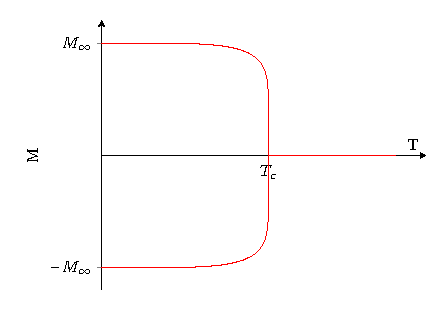
\includegraphics{Tikz Standalone/Tikz_magnetisierung.pdf}
\end{center}

\begin{itemize}
    \item[$\rightarrow$] Phasenübergang:
    \begin{itemize}
        \item $M$: Ordnungsparameter (genauer: $\expval{M}$)
        \item $T>T_c$: symmetrische oder ungeordnete Phase ($H$ ist rotationssymmetrisch, $S$ auch)
        \item $T<T_c$: spontane Symmetriebrechung,geringe Symmetrie, alle Spins ausgerichtet)
    \end{itemize}
    \item[$\rightarrow$] Physenübergang 2. Ordnung:
    \begin{itemize}
        \item Ordnungsparameter stetig (1. Ableitung unstetig)
        \item Phasen nicht gleichzeitig existent
        \item keine Umwandlungswärme notwendig
    \end{itemize}
    \item allgemein: \emph{Landau-Theorie der Phasenübergänge} (\say{Universalitätsklassen})
\end{itemize}

\paragraph{Ising-Modell}
\begin{center}
\emph{Motivation}: vollständig lösbares Modell des Ferromagnetismus mit Phasenübergang (\say{Es könnte ja sein, dass der Phasenübergang aus MFN resultiert.})
\end{center}
Heisenbergmodell ohne $x$- und $y$-Komponente des Spins:
\begin{equation}
    H = -g\mu_B B_z \sum_i S_i^z - J \sum_{\expval{i,j}} S_i^z S_j^z \qquad J > 0
\end{equation}
\begin{itemize}
    \item in diesem Modell alle Mikrozustände / Eigenzustände bekannt
    \item $S_i^z$ vertauschen mit Hamilton-Operator
    \begin{itemize}
        \item[$\Rightarrow$] Eigenzustände von $H$ sind beliebige Konfigurationen der Spins
        \begin{equation}
            \qq{mit} \ket{+} \ (\sigma = +1) \qq{oder} \ket{-} \ (\sigma = -1)
        \end{equation}
        \item[$\Rightarrow$] Energie einer Spinkonfiguration:
        \begin{equation}
            E(\{\sigma_i\}) = - \Tilde{B} \sum_i \sigma_i - \Tilde{J} \sum_{\expval{i,j}} \sigma_i\sigma_j
        \end{equation}
    \end{itemize}
    \item[1D]: exakte Lösung, kein Phasenübergang, kein Ferromagnetismus
    \item[2D]: Ising-Modell für $\Tilde{B}=0$
    \item[] Onsager 1944: (Zustandsumme + freie Energie)
    \begin{itemize}
        \item[$\Rightarrow$] Phasenübergang:
        \begin{equation}
            \sinh\left(\frac{2\Tilde{J}}{kT_c}\right) = 1 \qquad \Rightarrow \quad T_c = 2,269...\cdot \frac{\Tilde{J}}{k}
        \end{equation}
    \end{itemize}
    \item[] Young 1952:
    \begin{equation}
        M(T,B=0) \propto \expval{\sigma_i} = \begin{cases}
            \qquad \qq{0}\qquad \qq{      }, T>T_c\\
            \pm \left(1-\frac{1}{\sinh^4\left(\frac{2\Tilde{J}}{kT}\right)}\right)^{1/8} \ , T<T_c
        \end{cases}
    \end{equation}
\end{itemize}

\begin{center}
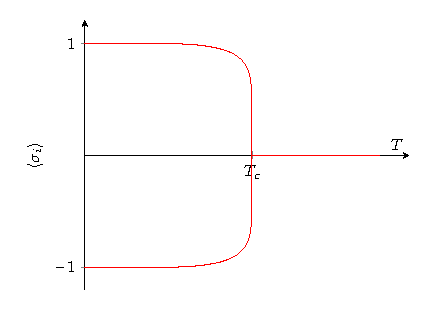
\includegraphics{Tikz Standalone/Tikz_spin.pdf}
\end{center}

Numerik:
\begin{itemize}
    \item dimensionslose Temperatur:
    \begin{align}
        \tau :&= \frac{T}{\frac{\Tilde{J}}{k}}\\
        \tau_c :&= \frac{T_c}{\frac{\Tilde{J}}{k}} = 2,269...
    \end{align}
\end{itemize}

\section{Transport-Gleichungen} \marginpar{VL 27}
\begin{itemize}
    \item[] bisher: Gleichgewicht $\widehat{=}$ \say{Thermostatistik}
    \item[] jetzt: Nicht-Gleichgewicht: Dynamik, Transport, Weg ins Gleichgewicht
\end{itemize}

\subsection{Boltzmann-Gleichung, H-Theorem}
\subsubsection*{Boltzmann-Gleichung}
verdünntes Gas mit $\lambda \ll \left(\frac{V}{N}\right)^{1/3} \quad \Rightarrow$ klassische Beschreibung

\paragraph{bisher:}
\begin{itemize}
    \item[] N-Teilchen Phasenraum: $(q_1,...,q_f,p_1,...,p_f) \qquad f= 3N$
    \item[] Mikrozustand: Punkt im 6N-dimensionalen Phasenraum
    \item[] Makrozustan: WS-Dichte $\varrho(q_1,...,q_f,p_1,...,p_f)$
\end{itemize}

\paragraph{jetzt:}
\begin{itemize}
    \item[] Einteilchen-Phasenraum $\Vec{q}, \Vec{p}$ mit f = 6
    \item[] Mikrozustand: N Punkte im Einteilchen-Phasenraum
    \item[] $\stackrel{\text{nähern}}{\longrightarrow}$ WS-Dichte $f(\Vec{q},\Vec{p},t)$ mit
    \begin{equation}
        f(\Vec{q},\Vec{p},t) \cdot d^3q \ d^3p \qq{Zahl der Teilchen im Volumen} d^3q \ d^3p
    \end{equation}
    \item[$\Rightarrow$] $\int \ f(\Vec{q},\Vec{p},t) \ d^3q d^3p \ = \ N$  
\end{itemize}

\paragraph{Ziel:} Bestimme $f(\Vec{q},\Vec{p},t)$ in Abhängigkeit von WW zwischen den Teilchen. \color{black!40} (deutlich einfacher als 6N-dim. Phasenraum, aber nicht vollst. Information; Reduktion bis auf 1D möglich) \color{black}

\paragraph{ohne WW:}
Hamilton-Bewegungsgleichung:
\begin{equation}
    \dot{\Vec{q}} = \pdv{H}{\Vec{p}} = \frac{\Vec{p}}{m} \qquad \dot{\Vec{p}} = - \pdv{H}{\Vec{q}} = \Vec{F} \qq{\color{black!40}(Kraft)\color{black}}
\end{equation}
Liouville-Theorme:
\begin{align}
    0 = \dv{f(\Vec{q},\Vec{p},t)}{t} &= \pdv{f}{t} + \pdv{f}{\Vec{q}} \Dot{\Vec{q}} + \pdv{f}{\Vec{p}} \Dot{\Vec{p}} \\
    &\Longrightarrow \left( \pdv{}{t} + \frac{\Vec{p}}{m} \pdv{}{\Vec{q}} + \Vec{F} \pdv{}{\Vec{p}} \right) f(\Vec{q},\Vec{p},t) = 0 \qq{stoßfreie Boltzmann-GL}
\end{align}
Sei:
\begin{itemize}
    \item $\Vec{F}=0$
    \item homogen im Ort $\Rightarrow \ f(\Vec{p},t)$
    \item[] $\Rightarrow \quad \pdv{f(\Vec{p},t)}{t}=0$
    \item[] $\Rightarrow$ jede zeitlich konstante Wahscheinlichkeitsdichte $f(\Vec{p})$ ist Lösung
    \item[] $\Rightarrow$ kein Weg ins GG ohne WW
\end{itemize}

\subsubsection*{mit WW:}
\begin{definition}{Boltzmann-Gleichung}
    \begin{equation}
    \left( \pdv{}{t} + \frac{\Vec{p}}{m} \pdv{}{\Vec{q}} + \Vec{F} \pdv{}{\Vec{p}} \right) f(\Vec{q},\Vec{p},t) = \left(\pdv{f(\Vec{q},\Vec{p},t)}{t}\right)_{\text{Stöße}}
    \end{equation}
\end{definition}

verdünntes Gas $\Rightarrow$ Stoßdauer $\ll$ Zeit zwischen Stößen $\Rightarrow$ nur 2-Teilchen-Stöße wichtig
\begin{figure}[h]
    \centering
    \begin{tikzpicture}
        \filldraw[fill=black!30, draw=black,thick] (0,0) circle (1);
        \draw[->] (-2,1) -- (-0.5,0.2);
        \draw (-2.2,0.7) node{$\Vec{p_1}$};
        \draw[->] (-2,-1) -- (-0.5,-0.2);
        \draw (-2.2,-0.7) node{$\Vec{p_2}$};
        \draw[->] (0.5,0.2) -- (2,1);
        \draw (2.2,0.7) node{$\Vec{p_1}^\prime$};
        \draw[->] (0.5,-0.2) -- (2,-1);
        \draw (2.2,-0.6) node{$\Vec{p_2}^\prime$};
    \end{tikzpicture}
\end{figure}

Zahl der Stoßpaare $\Vec{p}_1,\Vec{p}_2$ bei $\Vec{q}$:
\begin{align}
    dN = \underbrace{F(\Vec{q},\Vec{p}_1,\Vec{p}_2,t)}_{\substack{\text{2-Teilchen-Korrelationen,}\\ \text{unbekannt}}}\ d^3q \ d^3p_1 \ d^3p_2 \\
    \Rightarrow \quad \left(\pdv{f(\Vec{q},\Vec{p},t)}{t}\right)_{\text{Stöße}} = \int &\ d^3p_2 \ d^3p_1^\prime \ d^3p_1^\prime \cdot \underbrace{\delta^3(\Vec{p_1}^\prime + \Vec{p_2}^\prime - (\Vec{p}_1 + \Vec{p}_2)) }_{\text{Impulserhaltung}}\\
    &\cdot \underbrace{\delta\left(\frac{\abs{\Vec{p}_1^\prime}^2}{2m} + \frac{\abs{\Vec{p}_2^\prime}^2}{2m} - \left(\frac{\abs{\Vec{p}_1}^2}{2m} + \frac{\abs{\Vec{p}_2}^2}{2m}\right)\right)}_{\text{Energieerhaltung}} \\
    &\cdot \underbrace{\abs{T_{12\rightarrow1^\prime2^\prime}}^2}_{\text{qm. Streumatrixelement}} \\
    &\cdot \underbrace{\left(F(\Vec{q},\Vec{p}_1^\prime,\Vec{p}_2^\prime,t) - F(\Vec{q},\Vec{p}_1,\Vec{p}_2,t) \right)}_{\text{Zeitumkehr} \; (T_{12\rightarrow1^\prime2^\prime} = T_{1^\prime2^\prime\rightarrow12})}
\end{align}

Stoßzahlansatz (d.h. unkorrelierte Impulse):
\begin{align}
    F(\Vec{q},\Vec{p}_1,\Vec{p}_2,t) = \underbrace{f(\Vec{q},\Vec{p}_1,t)}_{=: f_1} &\cdot \underbrace{f(\Vec{q},\Vec{p}_2,t)}_{=: f_2} \\ \label{eq.Boltzmann}
    \left( \pdv{}{t} + \frac{\Vec{p}}{m} \pdv{}{\Vec{q}} + \Vec{F} \pdv{}{\Vec{p}} \right) f(\Vec{q},\Vec{p}_1,t) = \int &\ d^3p_2 \ d^3p_1^\prime \ d^3p_1^\prime \cdot \delta^3(\Vec{p}_f-\Vec{p}_i) \cdot \delta(E_f-E_i) \\
    &\cdot \abs{T_{i\rightarrow f}}^2 \cdot \left(f_1^\prime \cdot f_2^\prime -f_1\cdot f_2 \right)
\end{align}

\subsubsection*{H-Theorem}
Sei:
\begin{itemize}
    \item $\Vec{F}=0$
    \item homogen im Ort: $f=f(\Vec{p},t)$
    \item[$\Rightarrow$] linke Seite in \cref{eq.Boltzmann} nur $\pdv{}{t} f(\Vec{p}_1,t)$
\end{itemize}
Definiere nun (verwandt mit Entropie):
\begin{align}
    H(t) := \int \ d^3p_1 \ f(\Vec{p_1},t) \ \ln(f(\Vec{p}_1,t))
\end{align}

\begin{definition}{Boltzmann H-Theorem}
    \begin{equation}
        \dv{H(t)}{t} \leq 0
    \end{equation}
\end{definition}

\begin{proof}
\begin{align}\label{5_ableitung1}
    \dv{H}{t}&= \int \ d^3p_1 \ \pdv{f(\Vec{p_1},t)}{t} \left( \ln(f(\Vec{p}_1,t)) + 1\right)\\
    &= \int \ d^3p_1 \ d^3p_2 \ d^3p_1^\prime \ d^3p_2^\prime \ \delta^3(\Vec{p}_f-\Vec{p}_i)\cdot \delta(E_f-E_i)\cdot \abs{T_{i\rightarrow f}}^2 \\
    &\qquad \cdot (f_1^\prime f_2^\prime-f_1 f_2)\cdot (1+\ln(f(\Vec{p}_1,t)))
\end{align}
vertausche $\Vec{p}_1, \ \Vec{p}_2$:
\begin{align}\label{5_ableitung2}
    \dv{H}{t} = \int \ d^3p_1 \ d^3p_2 \ d^3p_1^\prime \ d^3p_2^\prime \ \delta^3(\Vec{p}_f-\Vec{p}_i)\cdot \delta(E_f-E_i)\cdot \abs{T_{i\rightarrow f}}^2 \\
    \qquad \cdot (f_1^\prime f_2^\prime-f_1 f_2)\cdot (1+\ln(f(\Vec{p}_2,t)))
\end{align}
addiere \cref{5_ableitung1} und \cref{5_ableitung2} und dividiere durch 2:
\begin{align}\label{5_ergebnis1}
    \dv{H}{t} = \int \ d^3p_1 \ d^3p_2 \ d^3p_1^\prime \ d^3p_2^\prime \ \delta^3(\Vec{p}_f-\Vec{p}_i)\cdot \delta(E_f-E_i)\cdot \abs{T_{i\rightarrow f}}^2 \\
    \qquad \cdot (f_1^\prime f_2^\prime-f_1 f_2)\cdot \frac{1}{2} \cdot (2+\ln(f_1f_2))
\end{align}
vertausche $\Vec{p}_1, \ \Vec{p}_2$ mit $\Vec{p}_1^\prime, \ \Vec{p}_2^\prime$:
\begin{align}\label{5_ableitung3}
    \dv{H}{t} = \int \ d^3p_1 \ d^3p_2 \ d^3p_1^\prime \ d^3p_2^\prime \ \delta^3(\Vec{p}_f-\Vec{p}_i)\cdot \delta(E_f-E_i)\cdot \abs{T_{i\rightarrow f}}^2 \\
    \qquad \cdot (f_1^\prime f_2^\prime-f_1 f_2)\cdot \frac{1}{2} \cdot (2+\ln(f_1^\prime f_2^\prime))
\end{align}
addiere \cref{5_ableitung3} zu \cref{5_ergebnis1}:
\begin{align}
    \Longrightarrow \ \dv{H}{t} = \frac{1}{4}\cdot \int \ d^3p_1 \ d^3p_2 \ d^3p_1^\prime \ d^3p_2^\prime \ \delta^3(\Vec{p}_f-\Vec{p}_i)\cdot \delta(E_f-E_i)\cdot \abs{T_{i\rightarrow f}}^2 \\
    \qquad \cdot \underbrace{(f_1^\prime f_2^\prime-f_1 f_2)}_{=: y-x} \cdot \underbrace{(\ln(f_1 f_2)+\ln(f_1^\prime f_2^\prime))}_{=: \ln x -\ln y}
\end{align}
nutze $(y-x)\cdot (\ln x -\ln y) \leq 0$ mit \say{=} falls $x=y$
\begin{equation}
    \Longrightarrow \; \dv{H}{t} \leq 0
\end{equation}
\end{proof}

\paragraph{Bemerkung:}
\begin{equation}
    \Dot{\Tilde{S}} = -k \cdot \Dot{H} \geq 0 \qq{Entropie wächst}
\end{equation}
\begin{itemize}
    \item ausgezeichnete Zeitrichtung
    \item Grund: Stoßzahlansatz (Impulse unkorreliert)
    \begin{itemize}
        \item nach Stoß: Korrelation $\rightarrow$ hier vernachlässigt
        \item Auszeichnung einer Zeitrichtung
        \item physikalisch dennoch sinnvoll (Empirie)
    \end{itemize}
\end{itemize}

\paragraph{Gleichgewicht:}
\begin{align}
    \dv{H}{t} = 0 \stackrel{x=y}{\Longleftrightarrow} f_0(\Vec{p}_1) f_0(\Vec{p}_2) = f_0(\Vec{p}_1^\prime) f_0(\Vec{p}_2^\prime) \\
    \Longrightarrow \underbrace{\ln(f_0(\Vec{p}_1)) + \ln(f_0(\Vec{p}_2))}_{\text{vor Stoß}} = \underbrace{\ln(f_0(\Vec{p}_1^\prime)) + \ln(f_0(\Vec{p}_2^\prime))}_{\text{nach Stoß}}
\end{align}
\begin{itemize}
    \item Erhaltungssatz im Gelichgewicht für beliebigen Stoß:
    \begin{equation}
        \Vec{p}_1,\ \Vec{p}_2 \ \longrightarrow \ \Vec{p}_1^\prime,\ \Vec{p}_2^\prime
    \end{equation}
    \item sonst nur Impulserhaltung $(\sim \Vec{p})$ und Energieerhaltung ($\sim \abs{\Vec{p}}^2$)
    \begin{align}
        \Rightarrow \ln(f_0(\Vec{p})) &= A + \Vec{B}\cdot \Vec{p} + C \cdot \abs{\Vec{p}}^2 \qq{(5 Konstanten: A, $\Vec{B}$, C)} \\
        f_0(\Vec{p}) &= D \exp{(-E(\Vec{p}-\Vec{F})^2)} \qq{(5 Konstanten: A, $\Vec{B}$, C)}\\
        &\rightarrow \ \text{Gauß-Verteilung $\widehat{=}$ Maxwell'scher Geschwindigkeitsverteilung}
    \end{align}
\end{itemize}

\subsection{Master-Gleichung} \marginpar{VL 28}
Beschreibt die Zeitentwicklung der WS mit DGL 1. Ordnung.
\subsubsection*{Isoliertes System} $H \ \Rightarrow$ Eigenzustände $\ket{l}$ sind stationär

\paragraph{Makroskopisches System:} Es gibt trotzdem Übergänge, da die Isolation nicht vollständig ist. Übergangsrate von $\ket{l}$ nach $\ket{m}$: $a_{ml} \geq 0$. Aus der Invarianz unter Zeitumkehr folgt: $a_{ml} = a_{lm}$. $a_{ml} = 0$ fast überall, da die Kopplung nur schwach ist, finden nur Übergänge zu energetisch nahen Zuständen statt: $a_{ml} = 0$ für $\abs{E_l-E_m}> \delta E$ (Unschärfe aufgrund unvollständiger Isolierung.\\
Wie ändert sich die WS $p_l$ in einem Zustand $\ket{l}$ zu sein im Zeitraum $\Delta t$?
\begin{align}
    \Delta p_l = \underbrace{- \sum_{m \neq l} a_{ml} \cdot \Delta t\cdot p_l}_{\text{Abnahme}} \underbrace{+ \sum_{m \neq 0} a_{ml} \cdot \Delta t \cdot p_m}_{\text{Zunahme}} \\
    \Rightarrow \ \dv{p_l(t)}{t} = \sum_m (a_{lm} p_m(t) - a_{ml} p_l(t))\\
    \color{black!40} \text{für m=0 Summand 0, daher Unterscheidung egal}\\
    \longrightarrow \text{Master-Gleichung für (fast) isoliertes System}
\end{align}
Das ist ein Postulat, da es auf \emph{Markov-Annahme} beruht ($\widehat{=}$ Übergänge hängen lediglich vom aktuellen Zustand nicht aber von der Vergangenheit des Systems ab). Die Zeitumkehrinvarianz gilt nicht für $p_l(t)$ (durch Markov-Annahme), es werden also irreversible Prozesse beschrieben (z.B. Weg ins GG).

\subsubsection*{Kopplung an Wärmebad}
\begin{itemize}
    \item System hat Eigenzustände $\ket{l}$ mit Energie $E_l$
    \item Bad hat Eigenzustände $\ket{L}$ mit Energie $E_L$
    \item Gesamtsystem = System + Bad + schwache Kopplung
    \item Basiszustände $\ket{l,L}$ mit Energie $E_{l,L} = E_l + E_L$ (keine Eigenzustände)
    \item $P_{l,L}$ sei WS für System in Zustand $\ket{l}$ und im Bad in Zustand $\ket{L}$    
\end{itemize}
Master-Gleichung für das Gesamtsystem:
\begin{align}\label{5_MG1}
    \dv{P_{l,L}}{t} &= \sum_{m,M} \left(a_{l,L,m,M}\cdot P_{m,M} - a_{m,M,l,L}\cdot P_{l,L} \right) \\
    \qq{mit} a_{l,L,m,M} &= a_{m,M,l,L} \qq{und} a_{l,L,m,M} = 0 \qq{für} \abs{E_{l,L}-E_{m,M}} > \delta E
\end{align}
Zeitentwicklung der WS $p_l = \sum_L P_{l,L}$ des Systems ist von Interesse. Nutze bedingte WS:
\begin{align}
    P_{l,L} &= p_l \cdot P_{L|_l}\\
    &\text{Annahme: kanonische Verteilung unabhängig von L:} \\
    &\frac{1}{Z} \cdot e^{-\beta(E_{tot}-E_l)} =: C\cdot e^{+\beta E_L} = C\cdot e^{\frac{E_l}{kT}} \qq{mit} E_L + E_l = E_{tot} \\
    &\Rightarrow \dv{p_l}{t} = \sum_L \dv{p_{l,L}}{t} \stackrel{(\ref{5_MG1})}{=} \sum_{m,M,L} (a_{l,L,m,M}\cdot P_{m,M}-a_{m,M,l,L}\cdot P_{l,L})\\
    &= \sum_m \Big[ \underbrace{\sum_{M,L} a_{l,L,m,M} \cdot C \cdot e^{\frac{E_m}{kt}}\cdot p_m}_{\substack{=: b_{lm} \\ \text{effektive Übergangsrate}}} - \underbrace{\sum_{M,L} a_{m,M,l,L}\cdot C \cdot e^{\frac{E_l}{kt}} \cdot p_l}_{\substack{=: b_{ml} \\ \text{effektive Übergangsrate}}} \Big]
\end{align}
\begin{definition}{Master-Gleichung für System mit Wärmebad}
\begin{equation}
    \dv{p_l}{t} = \sum_m (b_{lm} \cdot p_m - b_{ml}\cdot p_l)
\end{equation}
\end{definition}
$\rightarrow$ wie oben, aber mit anderer Symmetrie:
\begin{align}
    b_{lm} e^{-\frac{E_m}{kT}} = b_{ml}e^{-\frac{E_l}{kT}} \ \rightarrow \ \frac{b_{lm}}{b_{ml}} = e^{-\frac{E_l-E_m}{kT}}
\end{align}
\color{black!40} ($\rightarrow$ qualitativ: immer leichter im System zu niedrigerer Energie und im Bad zu höherer als umgekehrt) \color{black}\\
Gleichgewichtslösung der Master-Gleichung:
\begin{align}
    \dv{}{t} p_l^G \stackrel{!}{=} 0 \qquad \Rightarrow \ \underbrace{\sum_m b_{lm}\cdot p_m^G}_{\text{Zunahme}} = \underbrace{\sum_m b_{ml}\cdot p_l^G}_{\text{Abnahme}} \quad \forall l
\end{align}
$\rightarrow$ GG-Lösung: kanonische Verteilung für das System:
\begin{align}
    p_l^G &= \frac{1}{Z}e^{-\frac{E_l}{kT}}\\
    &\Rightarrow \ \fcolorbox{red}{white}{$b_{lm}\cdot p_m^G = b_{ml}\cdot p_l^G$} \qq{detailliertes GG}\\
    &\text{\color{black!40} (GG gilt für jedes Zustandspaar einzeln!)}
\end{align}
Der WS-Strom ist zwischen beliebigen Paaren $m, \ l$ ausgeglichen (nicht erst $\sum_m ...$).
\paragraph{Anwendungen:}
\begin{itemize}
    \item Systeme ohne GG (Heizung im Gebäude)
    \item zeitperiodisch getrieben (Quanten-)Systeme
    \begin{itemize}
        \item \say{non-equilibrium steady states} $\widehat{=}$ detailliertes GG gilt nicht mehr
    \end{itemize}
\end{itemize}

\end{document}

